\documentclass[12pt,letterpaper,oneside]{report}

% =========================
% Idioma y codificación
% =========================
\usepackage[utf8]{inputenc}
\usepackage[T1]{fontenc}
\usepackage{underscore}
\usepackage[spanish]{babel}

% =========================
% Tipografía y calidad
% =========================
\usepackage{lmodern}   % evita muchos warnings de fuentes en T1
\usepackage{microtype} % mejor justificación y corte de palabras

% =========================
% Página
% =========================
\usepackage[margin=1in]{geometry}

% =========================
% Gráficos y fondo de portada
% =========================
\usepackage{graphicx}
\usepackage{float}
\usepackage{eso-pic}   % para colocar imagen de fondo en portada
\usepackage{xcolor}
\usepackage{listings}
\usepackage[most]{tcolorbox}

% =========================
% Esquema visual (Overleaf, sin shell-escape)
% =========================
\definecolor{zineBlueDark}{HTML}{0F2A3B}
\definecolor{zineBlueMid}{HTML}{1C4E69}
\definecolor{zineBlueSoft}{HTML}{EAF3F8}
\definecolor{zineCodeBg}{HTML}{F7FAFC}
\definecolor{zineCodeFrame}{HTML}{C8D9E6}
\definecolor{zineTermBg}{HTML}{EEF4F7}
\definecolor{zineTermFrame}{HTML}{99B7CA}
\definecolor{zineOutBg}{HTML}{F3F7F2}
\definecolor{zineOutFrame}{HTML}{9EB99A}
\definecolor{zineOkBg}{HTML}{E6F5E9}
\definecolor{zineOkFrame}{HTML}{2E7D32}
\definecolor{zineFailBg}{HTML}{FDECEC}
\definecolor{zineFailFrame}{HTML}{B3261E}

\lstdefinestyle{zineListing}{
  basicstyle=\ttfamily\small,
  columns=fullflexible,
  keepspaces=true,
  showstringspaces=false,
  breaklines=true,
  breakatwhitespace=false,
  frame=none,
  extendedchars=true,
  literate=
    {á}{{\'a}}1 {é}{{\'e}}1 {í}{{\'i}}1 {ó}{{\'o}}1 {ú}{{\'u}}1
    {Á}{{\'A}}1 {É}{{\'E}}1 {Í}{{\'I}}1 {Ó}{{\'O}}1 {Ú}{{\'U}}1
    {ñ}{{\~n}}1 {Ñ}{{\~N}}1 {ü}{{\"u}}1 {Ü}{{\"U}}1
    {└}{{+}}1 {┌}{{+}}1 {┐}{{+}}1 {┘}{{+}}1 {├}{{+}}1 {┤}{{+}}1
    {│}{{|}}1 {─}{{-}}1
}

\newcommand{\inlineconcept}[1]{%
  \tcbox[
    on line,
    boxrule=0pt,
    arc=2pt,
    left=4pt,right=4pt,top=1pt,bottom=1pt,
    colback=zineBlueSoft,
    colframe=zineBlueSoft
  ]{\textbf{#1}}%
}

\newcommand{\inlinecommand}[1]{%
  \tcbox[
    on line,
    boxrule=0.4pt,
    arc=2pt,
    left=4pt,right=4pt,top=1pt,bottom=1pt,
    colback=zineCodeBg,
    colframe=zineCodeFrame
  ]{\texttt{#1}}%
}

\newcommand{\cmd}[1]{\inlinecommand{#1}}

\newcommand{\inlineok}[1][OK]{%
  \tcbox[
    on line,
    boxrule=0.5pt,
    arc=2pt,
    left=4pt,right=4pt,top=1pt,bottom=1pt,
    colback=zineOkBg,
    colframe=zineOkFrame
  ]{\textbf{#1}}%
}

\newcommand{\inlinefail}[1][FAIL]{%
  \tcbox[
    on line,
    boxrule=0.5pt,
    arc=2pt,
    left=4pt,right=4pt,top=1pt,bottom=1pt,
    colback=zineFailBg,
    colframe=zineFailFrame
  ]{\textbf{#1}}%
}

\tcbset{
  zineblock/.style={
    breakable,
    listing only,
    boxrule=0.5pt,
    arc=2pt,
    left=6pt,right=6pt,top=6pt,bottom=6pt,
    listing options={style=zineListing},
    fonttitle=\bfseries\small,
    coltitle=zineBlueDark
  }
}

\newtcblisting{terminalblock}{
  zineblock,
  title={Terminal},
  colback=zineTermBg,
  colframe=zineTermFrame
}

\newtcblisting{codeblock}{
  zineblock,
  title={Código},
  colback=zineCodeBg,
  colframe=zineCodeFrame
}

\newtcblisting{outputblock}{
  zineblock,
  title={Salida},
  colback=zineOutBg,
  colframe=zineOutFrame
}

\newtcolorbox{criticalnote}[1][]{
  breakable,
  boxrule=0.6pt,
  arc=2pt,
  left=6pt,right=6pt,top=6pt,bottom=6pt,
  colback=zineFailBg,
  colframe=zineFailFrame,
  title={Nota crítica},
  fonttitle=\bfseries\small,
  #1
}

% =========================
% Enlaces
% =========================
\usepackage[hidelinks]{hyperref}

% =========================
% Formato de títulos
% =========================
\usepackage{titlesec}

% Capítulos
\titleformat{\chapter}
  {\normalfont\bfseries\LARGE}
  {\thechapter.}
  {0.75em}
  {}
\titlespacing*{\chapter}{0pt}{1.5ex}{2.0ex}

% Secciones
\titleformat{\section}
  {\normalfont\bfseries\Large}
  {\thesection}
  {0.75em}
  {}
\titlespacing*{\section}{0pt}{1.25ex}{0.75ex}

% Subsecciones
\titleformat{\subsection}
  {\normalfont\bfseries\large}
  {\thesubsection}
  {0.75em}
  {}
\titlespacing*{\subsection}{0pt}{1.0ex}{0.5ex}

% =========================
% Párrafos y listas
% =========================
\setlength{\parindent}{0pt}
\setlength{\parskip}{0.6em}

\usepackage{enumitem}
\setlist[itemize]{topsep=0.4em, itemsep=0.2em, leftmargin=1.6em}
\setlist[enumerate]{topsep=0.4em, itemsep=0.2em, leftmargin=1.6em}

% =========================
% Figuras y tablas (estilo consistente)
% =========================
\usepackage{caption}
\captionsetup{
  font=small,
  labelfont=bf,
  textfont=small
}

% Carpeta base para imágenes
\graphicspath{{images/}}

% =========================
% Variables del documento
% =========================
\newcommand{\ManualTitulo}{Manual de uso del clúster HPC}
\newcommand{\ManualInstitucion}{Universidad Javeriana}
\newcommand{\ManualVersion}{Versión 0.1}
\newcommand{\ManualFecha}{\today}

% Autores (4)
\newcommand{\AutorA}{Juan Guillermo Torres}
\newcommand{\AutorB}{Juan Manuel Mendoza}
\newcommand{\AutorC}{Juan Carlos Barrero}
\newcommand{\ManualAutores}{%
  \AutorA\\[0.25cm]
  \AutorB\\[0.25cm]
  \AutorC\\[0.25cm]
  % \AutorD%
}

% Portada: ruta del fondo y color del texto
% Recomendación: subir la imagen a images/portada/portada.png
\newcommand{\PortadaFondo}{images/portada/portada.png}
\newcommand{\PortadaTextoColor}{white} % white si el fondo es oscuro, black si es claro

% =========================
% Bibliografía global (al final del documento)
% =========================
% URLs (reduce overfull hbox)
\usepackage{xurl}

% Bibliografía global
\usepackage[backend=biber,style=ieee]{biblatex}
\addbibresource{bib/references.bib}

% Recomendado por biblatex con babel
\usepackage{csquotes}



\begin{document}

% Portada
% Valores por defecto (por si main.tex no los define todavía)
\providecommand{\ManualTitulo}{Manual de uso del clúster HPC}
\providecommand{\ManualSubtitulo}{Automatización con Ansible}
\providecommand{\ManualInstitucion}{Nombre de la institución / laboratorio}
\providecommand{\ManualVersion}{Versión 0.1}
\providecommand{\ManualFecha}{\today}

% Autores (4)
\providecommand{\AutorA}{Autor 1}
\providecommand{\AutorB}{Autor 2}
\providecommand{\AutorC}{Autor 3}
\providecommand{\AutorD}{Autor 4}
\providecommand{\ManualAutores}{%
  \AutorA\\[0.25cm]
  \AutorB\\[0.25cm]
  \AutorC\\[0.25cm]
  \AutorD%
}

% Fondo y color del texto en portada
\providecommand{\PortadaFondo}{images/portada/portada.png}
\providecommand{\PortadaTextoColor}{white}


\begin{titlepage}
\thispagestyle{empty}

% Fondo de portada (si el archivo existe)
\IfFileExists{\PortadaFondo}{%
  \AddToShipoutPictureBG*{%
    \AtPageLowerLeft{%
      \includegraphics[width=\paperwidth,height=\paperheight]{\PortadaFondo}%
    }%
  }%
}{}

% Color del texto en portada (definido en main.tex)
\color{\PortadaTextoColor}

\vspace*{2.2cm}

\begin{center}
  {\Huge\bfseries \ManualTitulo \par}
  \vspace{0.8cm}
  {\Large \ManualSubtitulo \par}
  \vspace{1.2cm}

  {\large \ManualInstitucion \par}
  \vfill

  {\large\bfseries Autores \par}
  \vspace{0.4cm}
  {\large \ManualAutores \par}
  \vfill

  {\large \ManualVersion \par}
  \vspace{0.2cm}
  {\large \ManualFecha \par}
\end{center}

\end{titlepage}


% Índices
\tableofcontents
\clearpage
\listoffigures
\clearpage
\listoftables
\clearpage

% =========================
% Capítulos
% =========================
\chapter{Configuración del entorno}
\label{chap:config_entorno}

Este capítulo describe la configuración base del clúster HPC desde un punto cero: descarga del sistema operativo, creación del medio de instalación, arranque del equipo, instalación de Rocky Linux y verificaciones iniciales.

\section{Preparación del medio de instalación (ISO y USB)}
\label{sec:iso_usb}

En esta etapa se prepara el sistema operativo que se instalará en el clúster. Para este proyecto se utiliza Rocky Linux 9.x, ya que corresponde a una rama estable con soporte a largo plazo. En la guía oficial de versiones se indica que Rocky Linux 9 tiene ciclo de vida planificado hasta 2032. \cite{rocky_version_guide}

Se eligió Rocky Linux 9.x (en lugar de Rocky Linux 10) por dos motivos prácticos. Primero, se buscó priorizar estabilidad y madurez de la plataforma en un entorno HPC donde los cambios de versión pueden introducir diferencias de compatibilidad y configuración. Segundo, en la documentación de notas de versión se describe que Rocky 10 soporta la arquitectura \texttt{x86\_64\_v3}; esto puede ser relevante si el hardware disponible incluye equipos que no cumplen ese nivel de instrucción, por lo que Rocky 9 reduce el riesgo de incompatibilidades de arranque o instalación en equipos heterogéneos. \cite{rocky_version_guide,rocky_release_notes}

\subsection{Descarga de la ISO de Rocky Linux 9.x Minimal}
Una imagen \textit{ISO} es el archivo que contiene el instalador completo del sistema operativo. En este proyecto se utilizó la imagen \textbf{Minimal ISO} de Rocky Linux 9.x para estandarizar la instalación base del clúster y reducir componentes innecesarios en servidores. La página oficial de descargas ofrece la opción \textit{Minimal ISO} para Rocky Linux 9. \cite{rocky_download}

\subsubsection*{Procedimiento realizado}
\begin{enumerate}
  \item Se ingresó a la página oficial de descargas de Rocky Linux.
  \item Se seleccionó la familia \textbf{Rocky Linux 9} y la arquitectura \textbf{AMD/Intel (\texttt{x86\_64})}.
  \item Se descargó la imagen \textbf{Minimal ISO}. En el repositorio oficial de imágenes, esta imagen aparece como \texttt{Rocky-9-latest-x86\_64-minimal.iso}. \cite{rocky_9_isos}
\end{enumerate}

\begin{figure}[H]
    \centering
    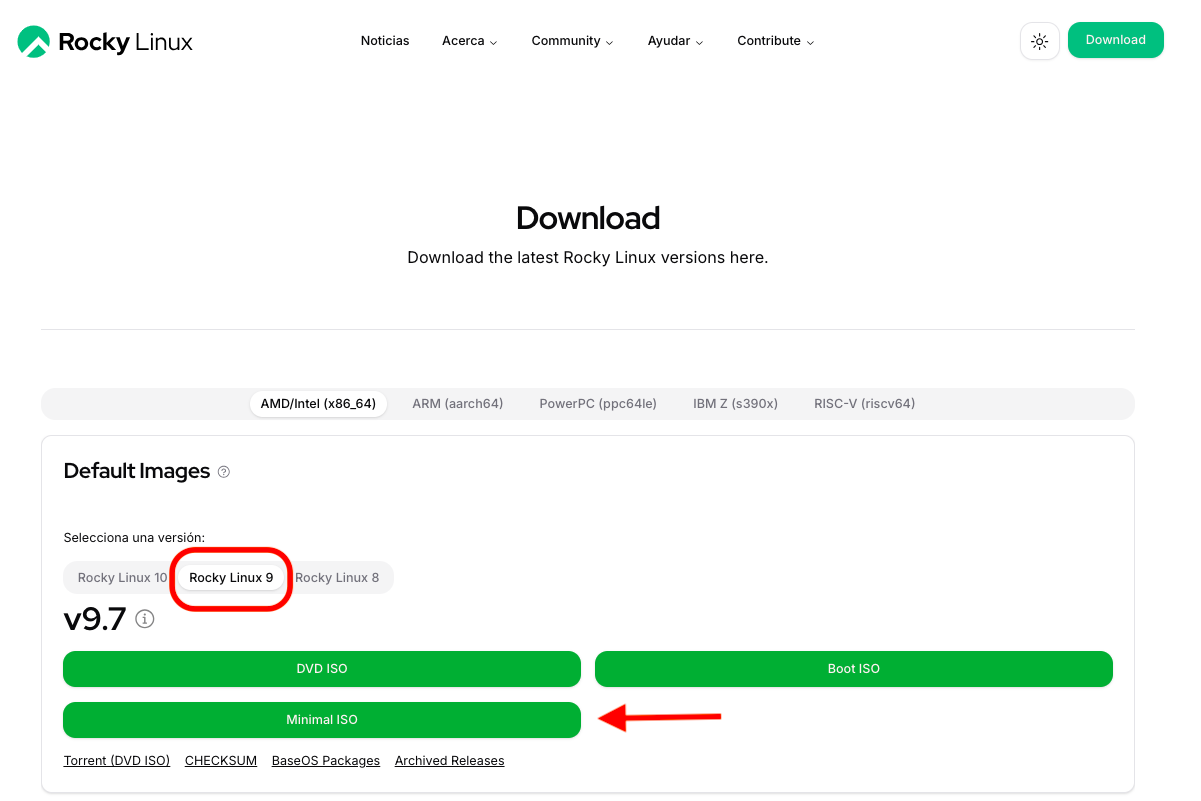
\includegraphics[width=0.95\linewidth]{images/HPC/SO/Rocky Dwl.png}
    \caption{Página de descarga de Rocky 9.x}
    \label{fig:rocky_web_dwl}
\end{figure}

\begin{figure}[H]
    \centering
    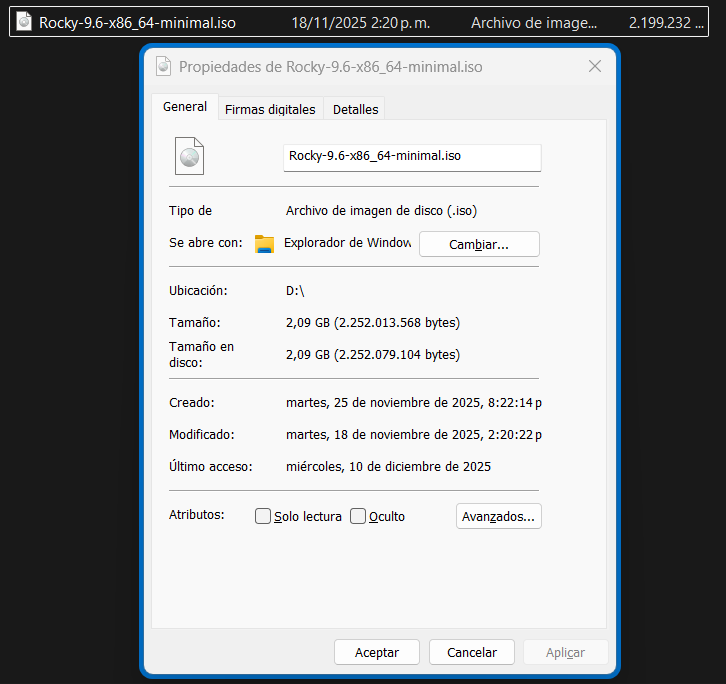
\includegraphics[width=0.5\linewidth]{images/HPC/SO/ISO Rocky 9x.png}
    \caption{Rocky-9.6-x86\_64-minimal.iso}
    \label{fig:iso_rocky}
\end{figure}

Al finalizar la descarga, el archivo ISO quedó disponible localmente con el nombre \texttt{Rocky-9.x-x86\_64-minimal.iso} (o un nombre equivalente si el navegador añadió sufijos), y con un tamaño del orden de gigabytes, coherente con una imagen de instalación. \cite{rocky_9_isos}

\subsection{Preparación de la USB booteable con Ventoy}
Una USB \textit{booteable} permite que el computador arranque desde la memoria USB y ejecute el instalador. Para este proyecto se utilizó Ventoy porque permite mantener una USB multipropósito: una vez instalado Ventoy en la USB, basta con copiar el archivo ISO a la partición principal sin tener que “flashear” la memoria cada vez. La documentación oficial de Ventoy indica que el usuario solo necesita copiar las imágenes (\textit{ISO}, entre otros formatos) a la primera partición y Ventoy las listará automáticamente en el menú de arranque. \cite{ventoy_start,ventoy_home}

\subsubsection*{Procedimiento realizado}
\begin{enumerate}
  \item Se conectó una memoria USB al computador utilizado para preparar el instalador.
  \item Se descargó el software Ventoy desde su página oficial \hyperlink{https://www.ventoy.net/en/download.html}{https://www.ventoy.net/en/download.html}

  \begin{figure}[H]
      \centering
      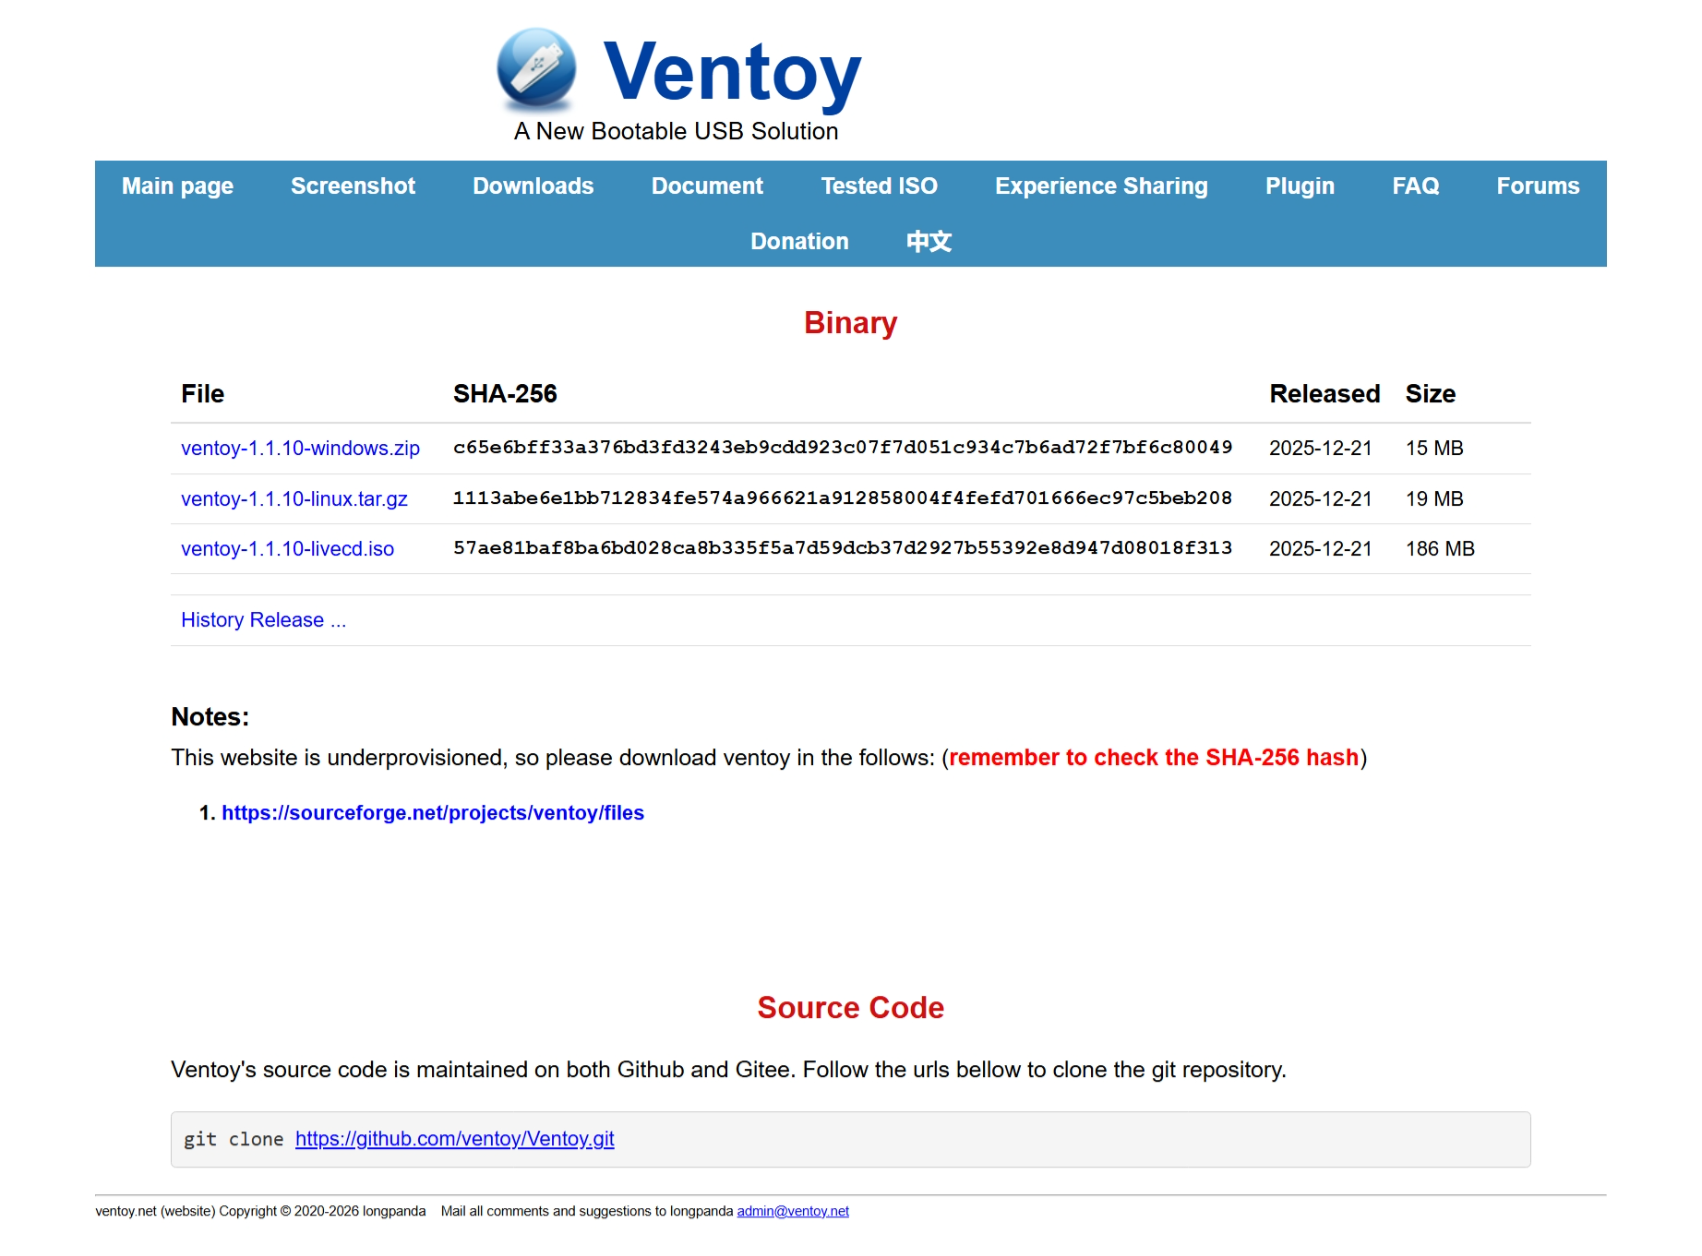
\includegraphics[width=0.75\linewidth]{images/Ventoy/ventoy dwl.png}
      \caption{Página de descarga oficial de Ventoy}
      \label{fig:ventoy_dwl_web}
  \end{figure}
  
  \item Se instaló Ventoy en la memoria USB (proceso que crea una partición principal donde se almacenan las ISOs). \cite{ventoy_start}

  \begin{figure}[H]
      \centering
      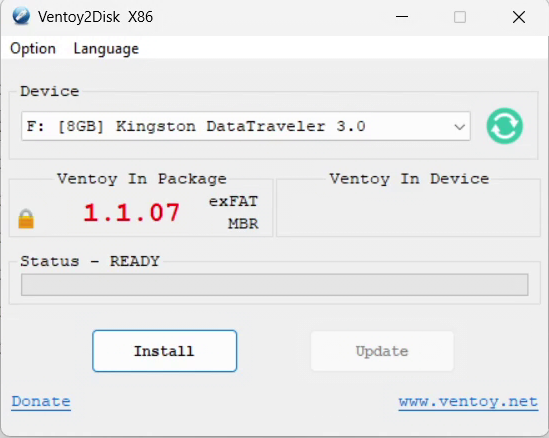
\includegraphics[width=0.5\linewidth]{images/Ventoy/Ventoy2Disk.png}
      \caption{Ventana del ejecutable de Ventoy (Ventoy2Disk.exe)}
      \label{fig:ventoy2disk}
  \end{figure}

  \begin{figure}[H]
      \centering
      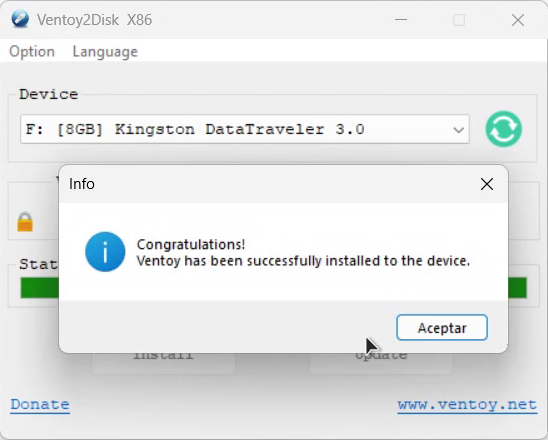
\includegraphics[width=0.5\linewidth]{images/Ventoy/inst message.png}
      \caption{Proceso de instalación de Ventoy terminado}
      \label{fig:ventoy inst}
  \end{figure}
  
  \item Se copió el archivo \texttt{Rocky-9.x-x86\_64-minimal.iso} a la partición principal de la USB (la partición usada para almacenar ISOs). \cite{ventoy_start,ventoy_home}

  \begin{figure}[H]
      \centering
      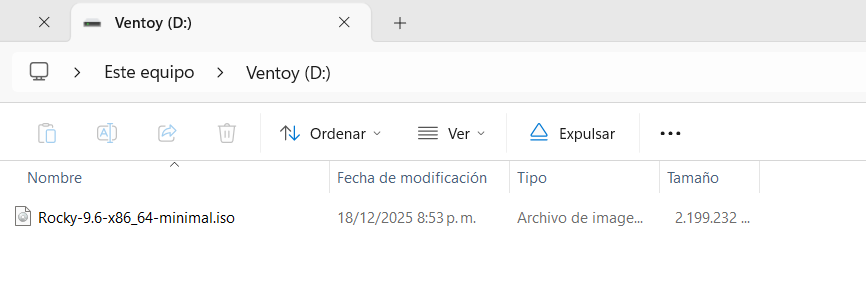
\includegraphics[width=0.95\linewidth]{images/Ventoy/ISO en ventoy.png}
      \caption{Directorio raíz de la USB con Ventoy}
      \label{fig:usb_iso}
  \end{figure}

  
\end{enumerate}

 En Ventoy, las imágenes pueden ubicarse en cualquier carpeta dentro de la partición principal y aun así aparecerán en el menú. \cite{ventoy_start}

\section{Instalación de Rocky Linux 9.x en el nodo master}
\label{subsec:instalacion_master}

En esta etapa se arranca el equipo desde la USB y se instala Rocky Linux 9.x en el nodo \textit{master}. Rocky Linux usa el instalador \textit{Anaconda}, que agrupa las decisiones de instalación en una pantalla principal llamada \textit{Resumen de instalación} (idioma, teclado, hora, software, disco y red). \cite{rocky_install_9_6}

\subsubsection*{Ingreso al menú de arranque y selección de la USB}
Se usa el menú de arranque de una sola vez para iniciar desde la USB sin alterar permanentemente el orden de arranque del equipo. En equipos Dell, el menú de arranque se abre presionando \texttt{F12} inmediatamente al encender o reiniciar. \cite{dell_f12_boot_menu}

\begin{enumerate}
  \item Se conectó la USB con Ventoy al equipo \textit{master}.
  \item Se encendió (o reinició) el equipo y se presionó \texttt{F12} para abrir el menú de arranque.

\begin{figure}[H]
  \centering
  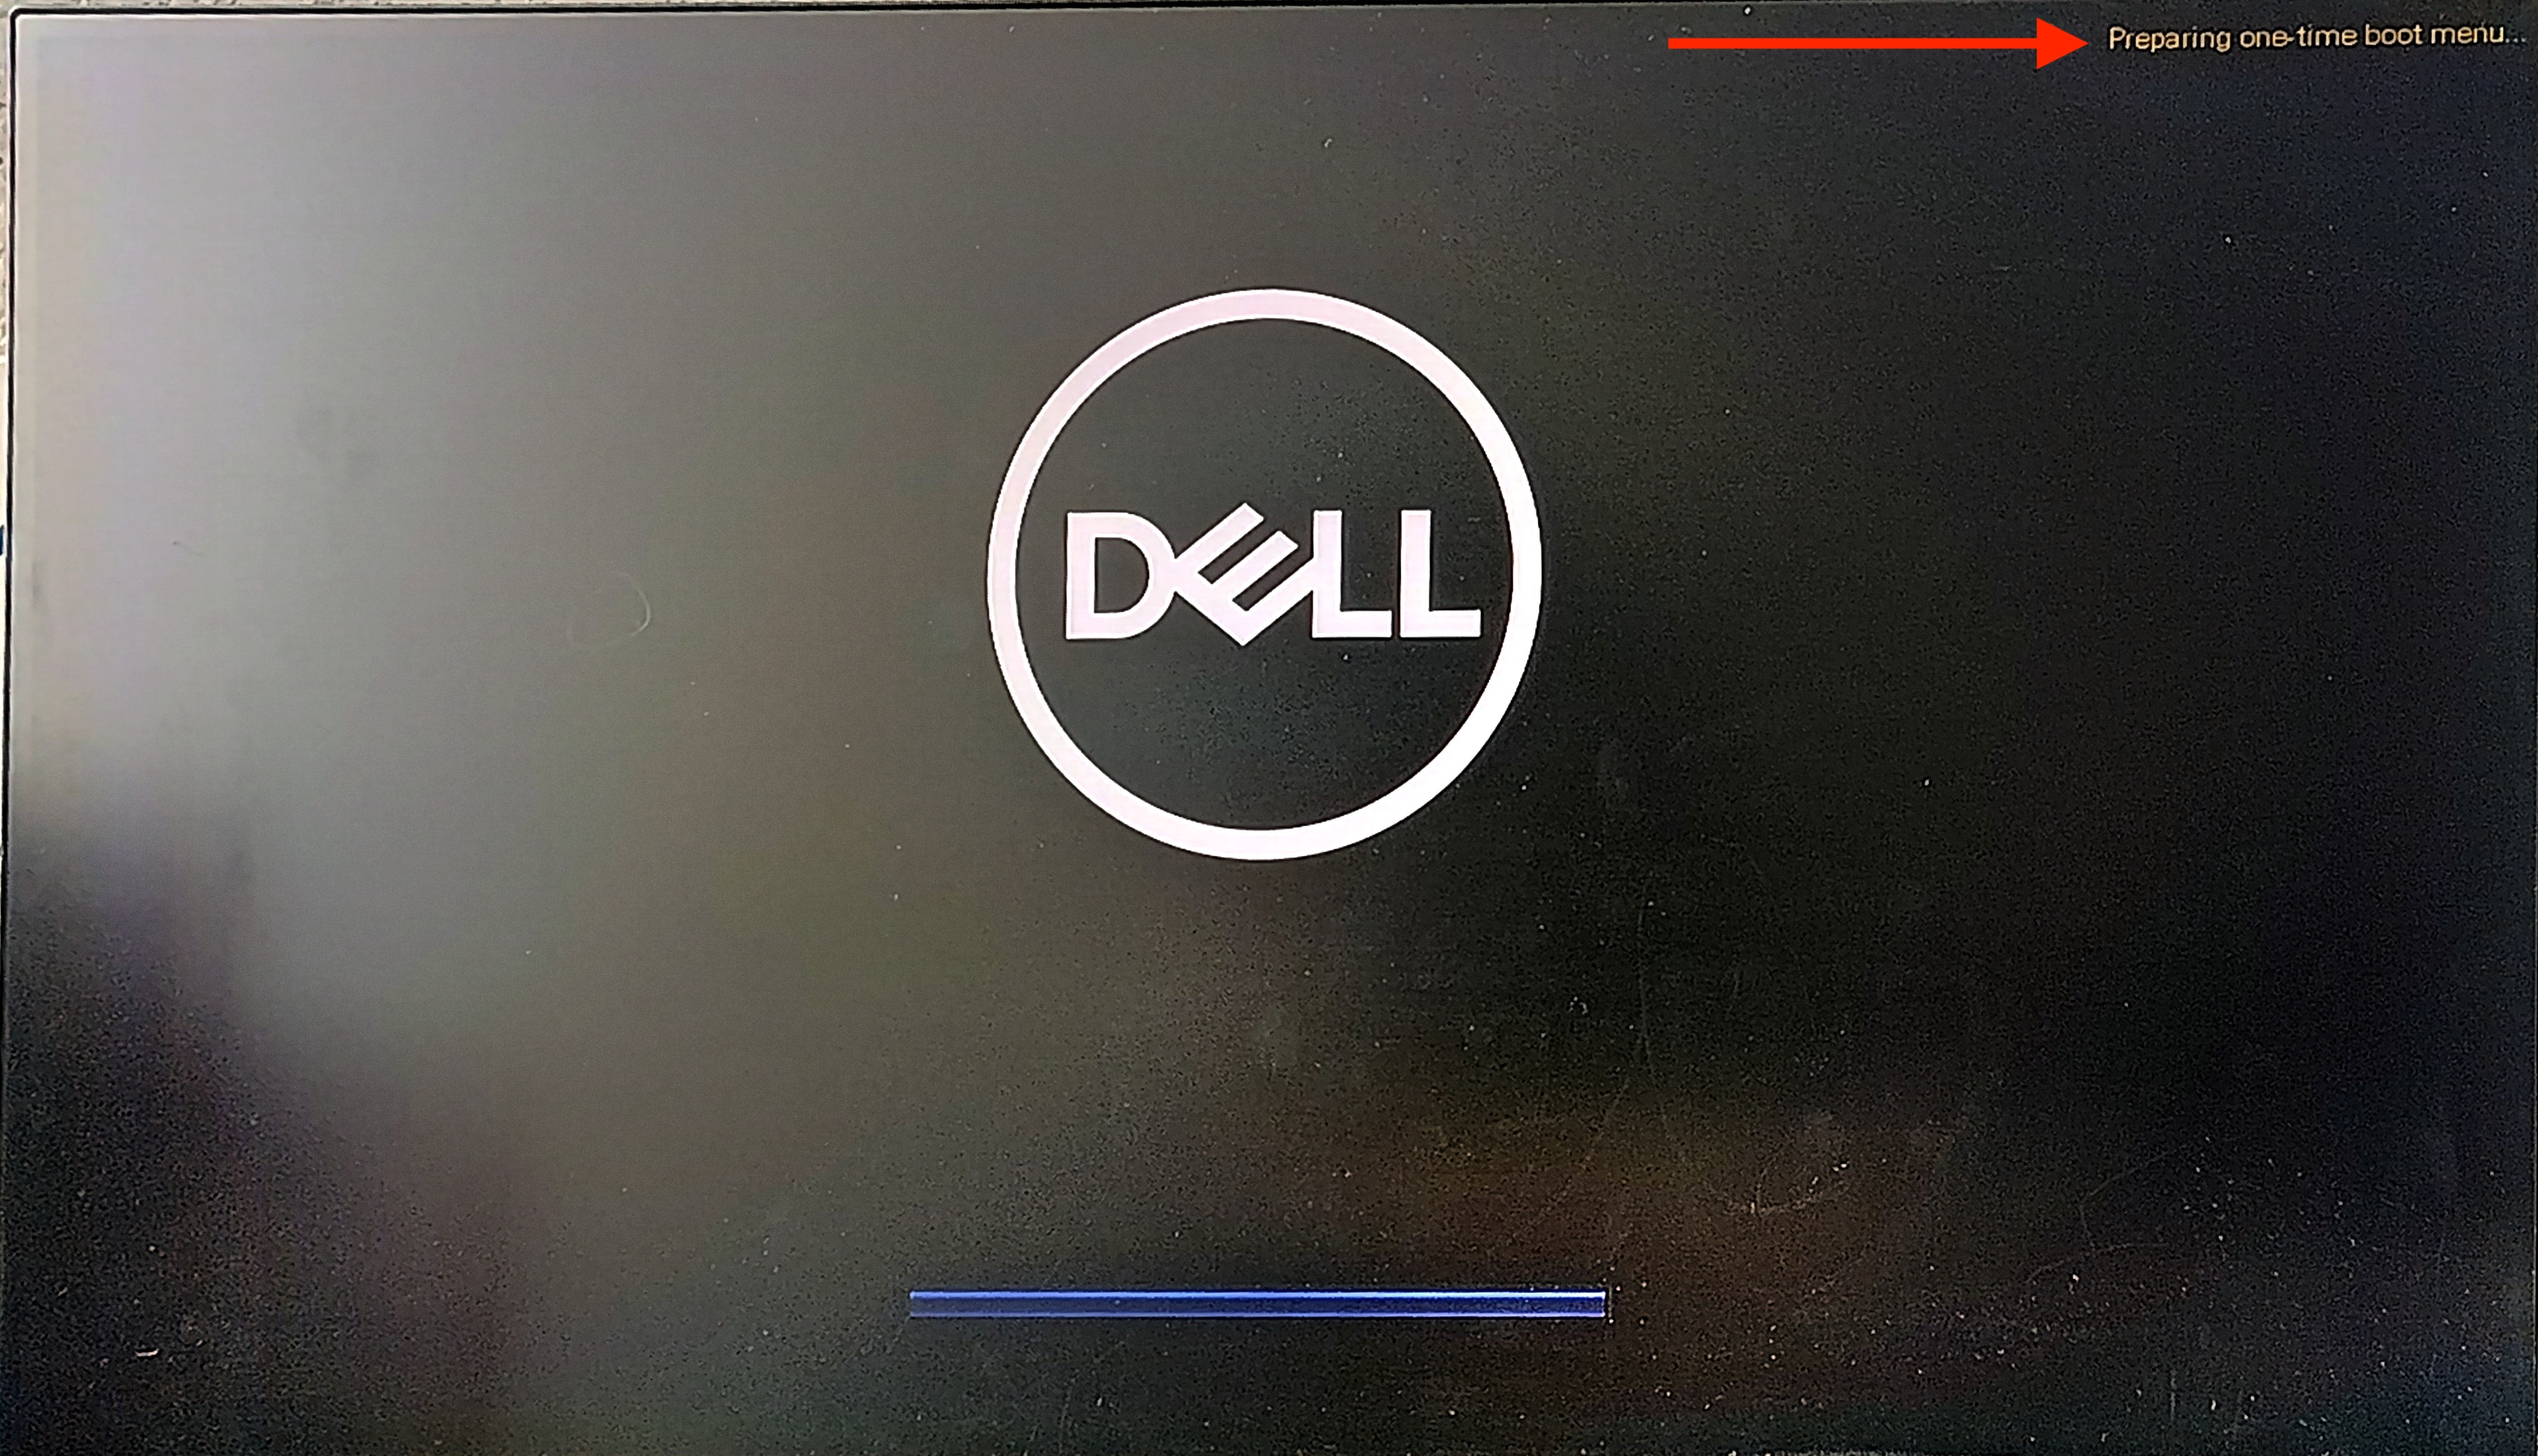
\includegraphics[width=0.92\textwidth]{images/HPC/SO/0_boot_screen.jpg}
  \caption{Pantalla de inicio del boot.}
  \label{fig:boot_start}
\end{figure}
  
  \item Se seleccionó la opción correspondiente a la USB.
\end{enumerate}

\begin{figure}[H]
  \centering
  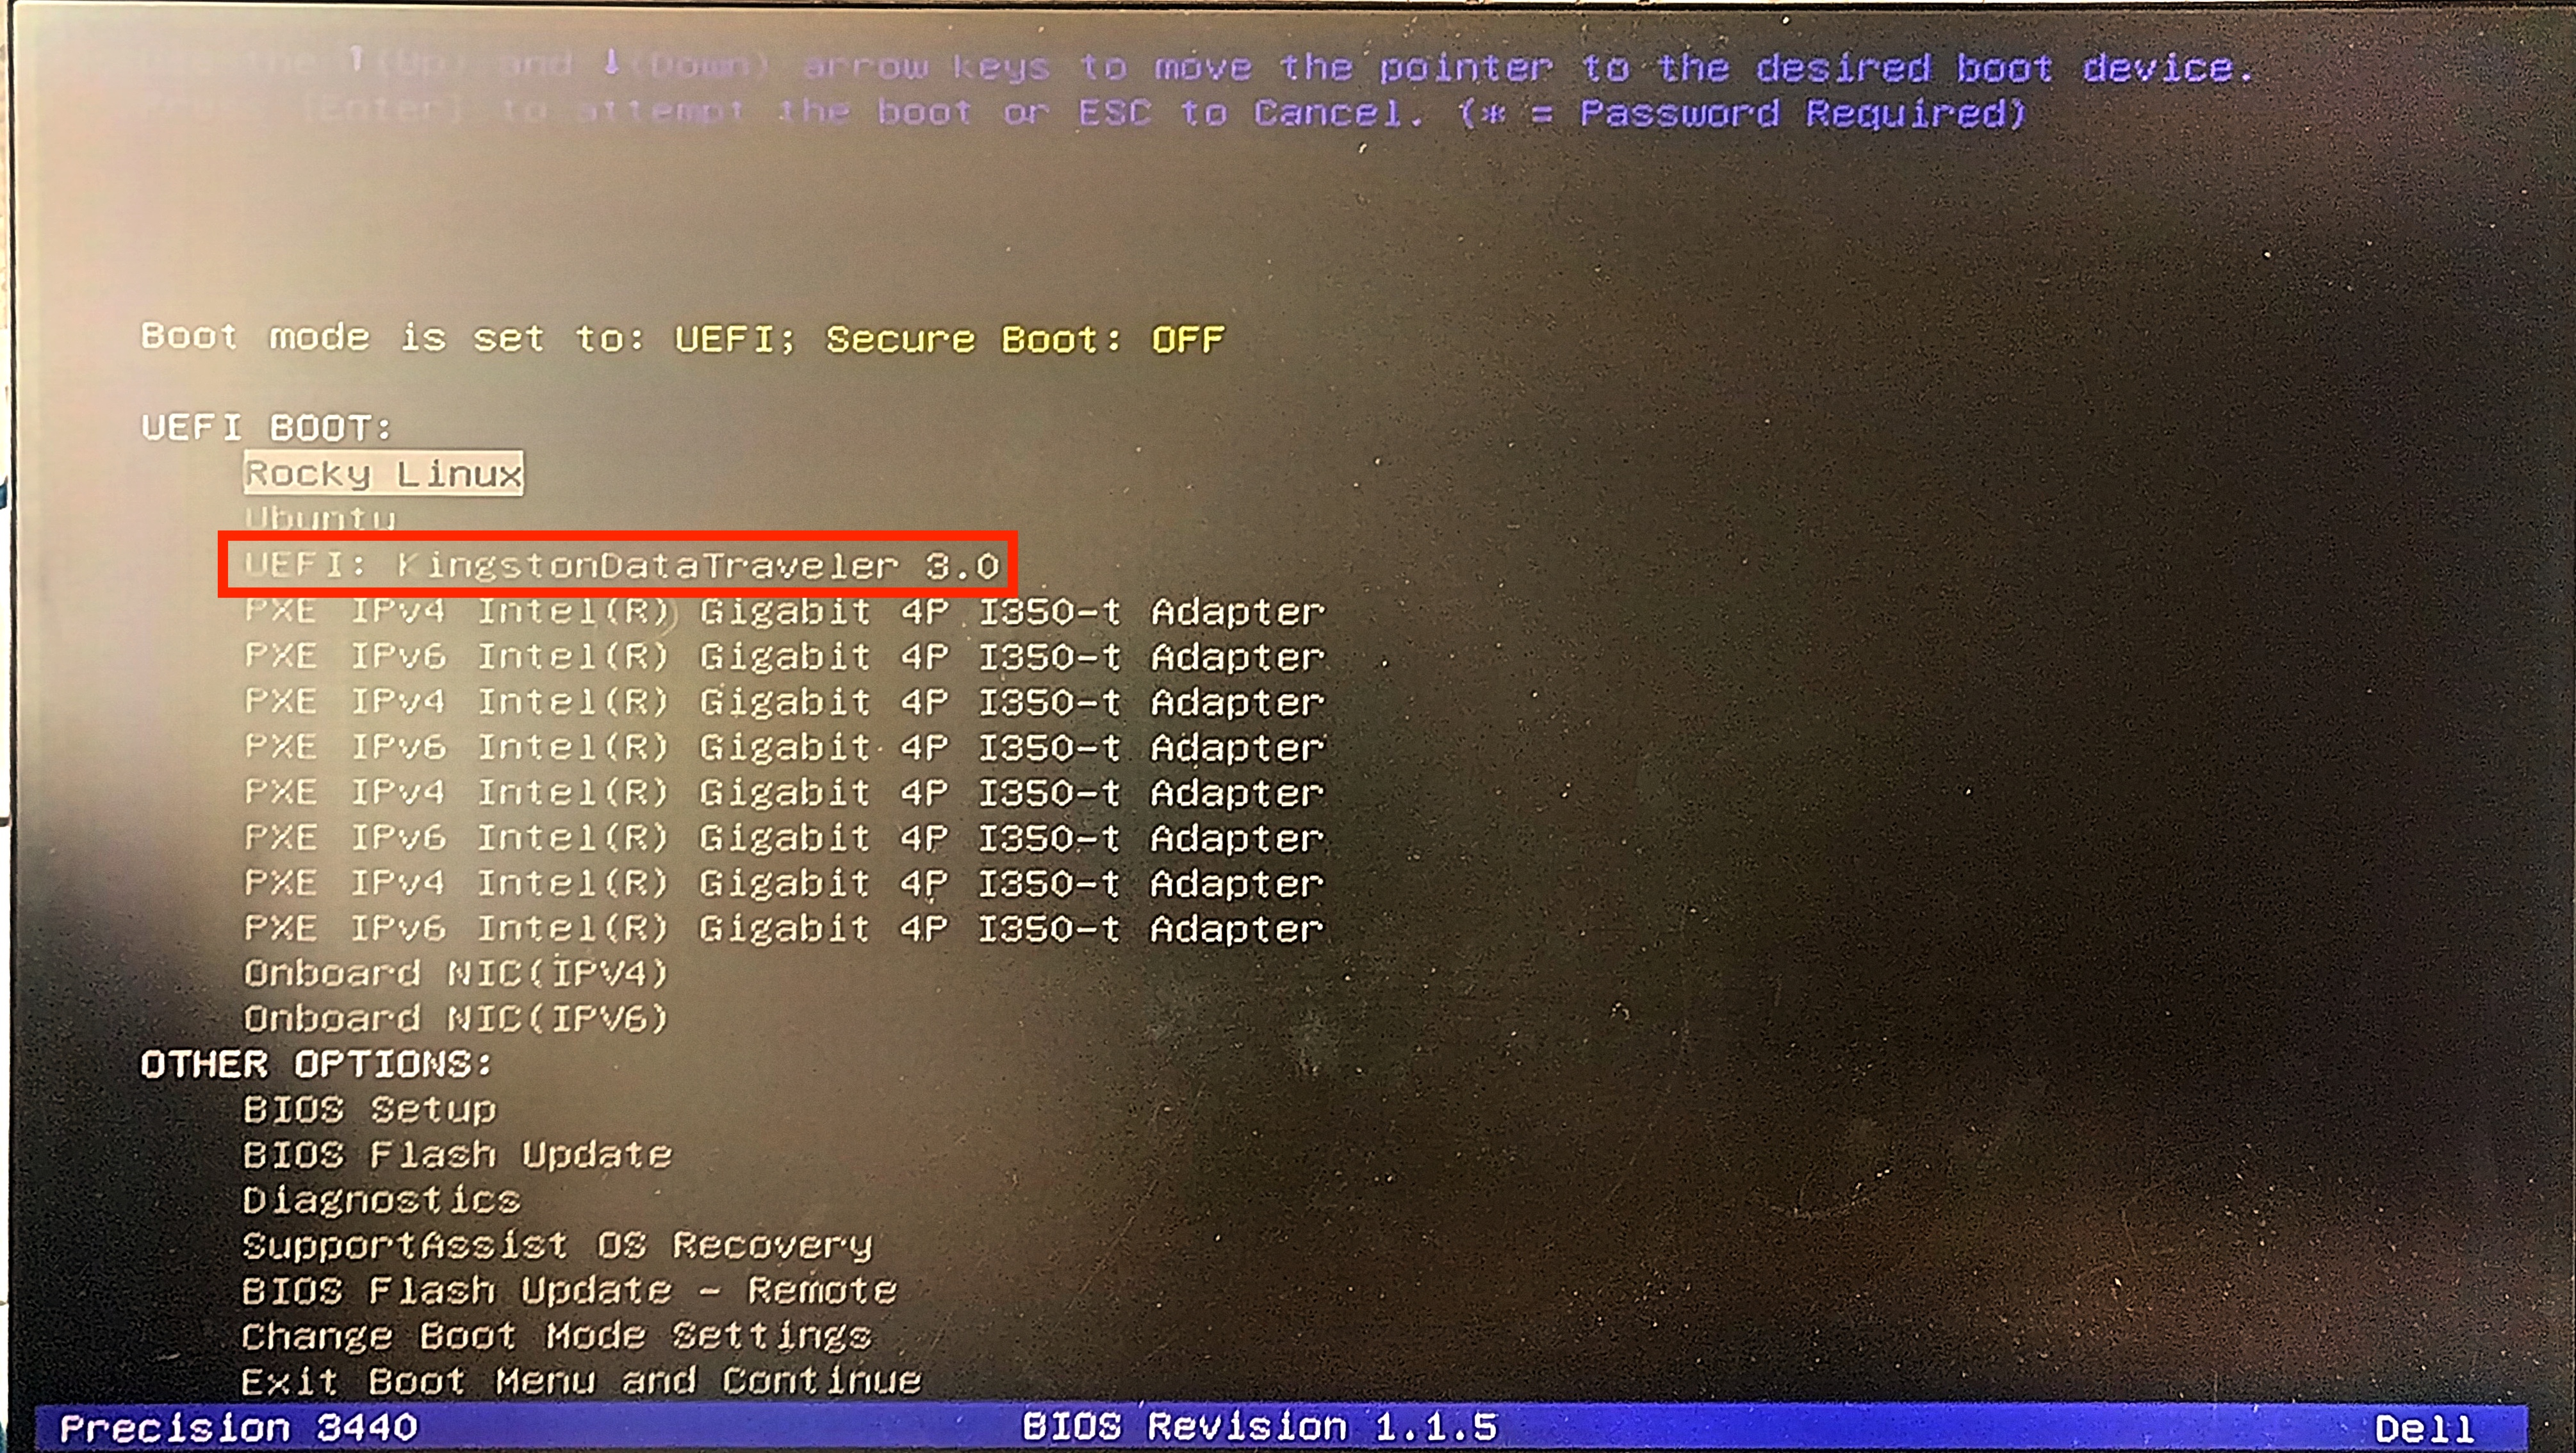
\includegraphics[width=0.92\textwidth]{images/HPC/SO/01_boot_menu_f12.jpg}
  \caption{Menú de arranque (F12) con la USB.}
  \label{fig:boot_menu_f12}
\end{figure}

Después de seleccionar la USB, se mostró el menú de Ventoy con el listado de imágenes disponibles. Ventoy detecta automáticamente los archivos ISO copiados en la partición principal y los lista en el menú de arranque. \cite{ventoy_start}

\begin{figure}[H]
  \centering
  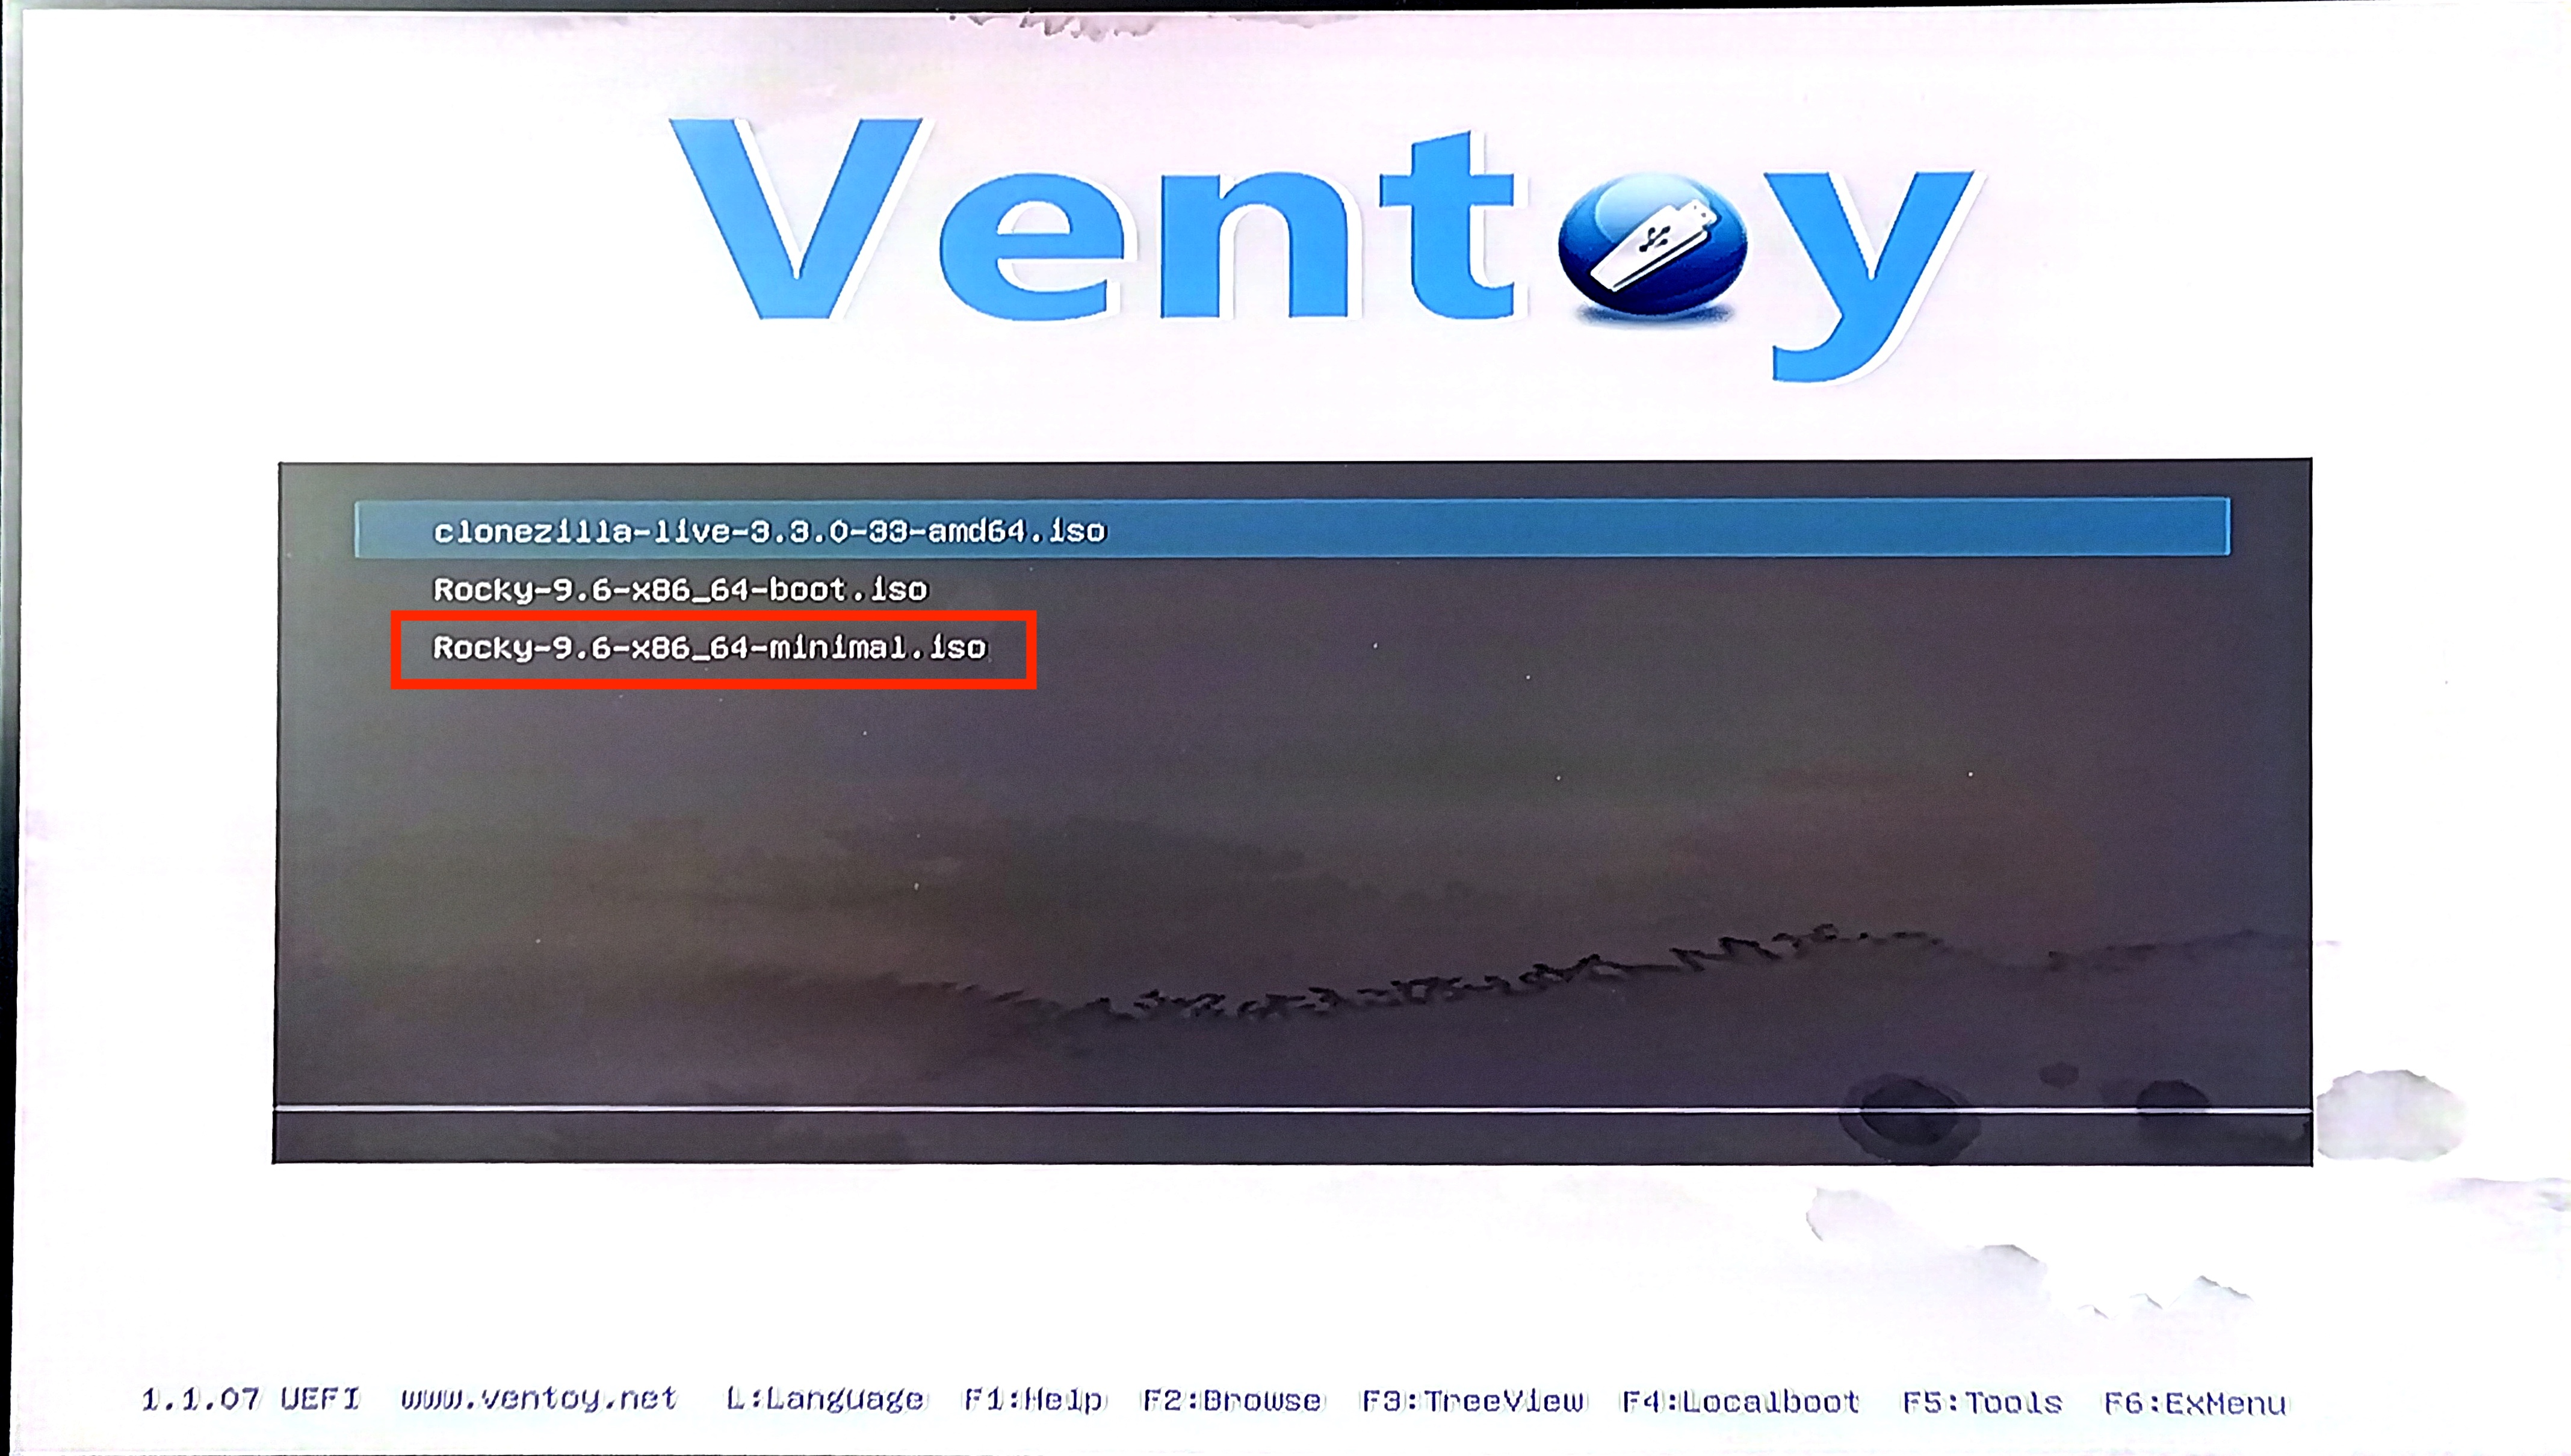
\includegraphics[width=0.92\textwidth]{images/HPC/SO/02_ventoy_menu1.jpg}
  \caption{Menú de Ventoy listando la ISO de Rocky Linux 9.x.}
  \label{fig:ventoy_menu1}
\end{figure}

\begin{figure}[H]
  \centering
  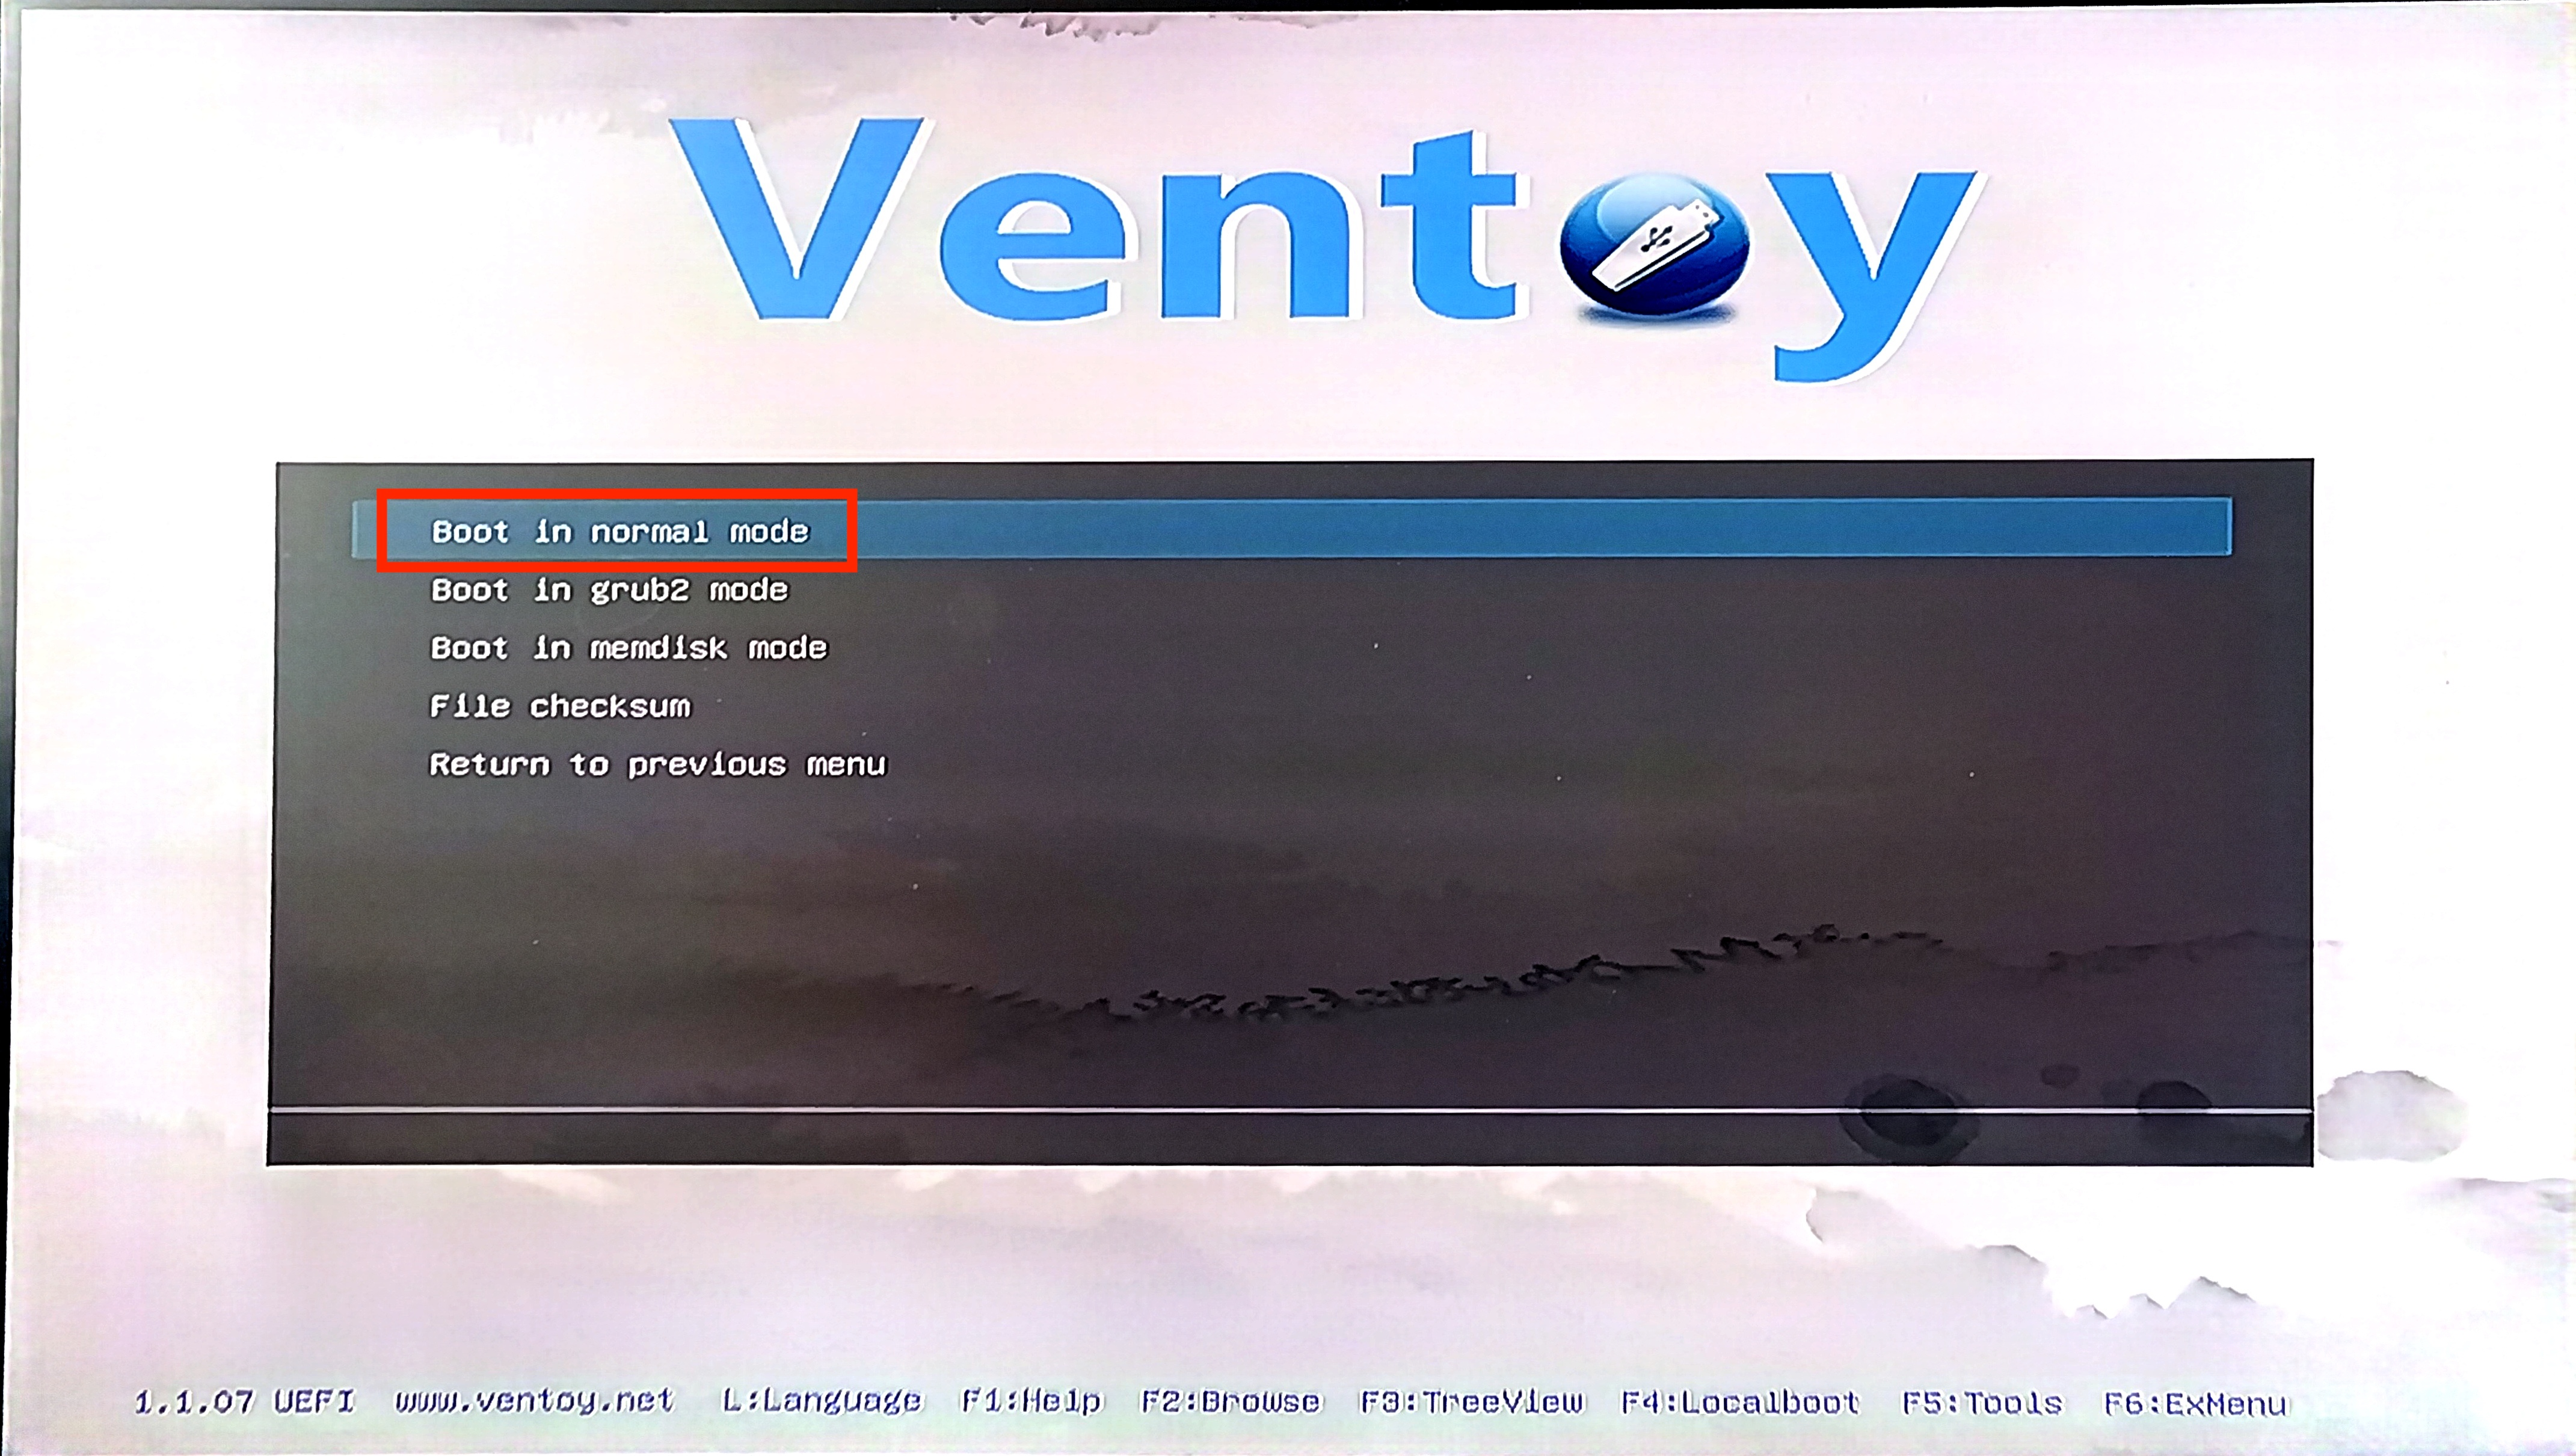
\includegraphics[width=0.92\textwidth]{images/HPC/SO/02_ventoy_menu2.jpg}
  \caption{Menú de Ventoy listando la ISO de Rocky Linux 9.x.}
  \label{fig:ventoy_menu2}
\end{figure}

\subsubsection*{Inicio del instalador desde la ISO}
\begin{enumerate}
  \item En el menú de Ventoy, se seleccionó la imagen \texttt{Rocky-9.6-x86\_64-minimal.iso}.
  \item Se confirmó el arranque desde la imagen seleccionada.
\end{enumerate}

% \begin{figure}[H]
%   \centering
%   \includegraphics[width=0.92\textwidth]{images/configuración_del_entorno/03_rocky_boot_menu.png}
%   \caption{Pantalla inicial del instalador de Rocky Linux al arrancar desde la ISO.}
%   \label{fig:rocky_boot_menu}
% \end{figure}

A continuación, se inició el instalador. Como verificación preventiva del medio, se utilizó la opción de prueba del medio cuando estuvo disponible (\textit{Test this media \& install}), con el fin de reducir el riesgo de fallas por corrupción del archivo o de la USB durante la instalación. \cite{rocky_install_9_6}

% \begin{figure}[H]
%   \centering
%   \includegraphics[width=0.92\textwidth]{images/configuración_del_entorno/04_test_media.png}
%   \caption{Opción de prueba del medio (\textit{Test this media \& install}).}
%   \label{fig:test_media}
% \end{figure}

Cuando la verificación finalizó correctamente, el instalador continuó a la selección de idioma. Esto confirmó, en la práctica, que el medio era utilizable para instalar.

\subsubsection*{Selección de idioma, teclado y zona horaria}
Estas opciones se configuran para que el sistema quede listo para el uso cotidiano y para que los registros del sistema (\textit{logs}) tengan hora correcta, lo cual es clave para auditoría y solución de problemas.

\begin{enumerate}
  \item Se seleccionó el idioma de instalación en Español y se continuó.
\end{enumerate}

\begin{figure}[H]
  \centering
  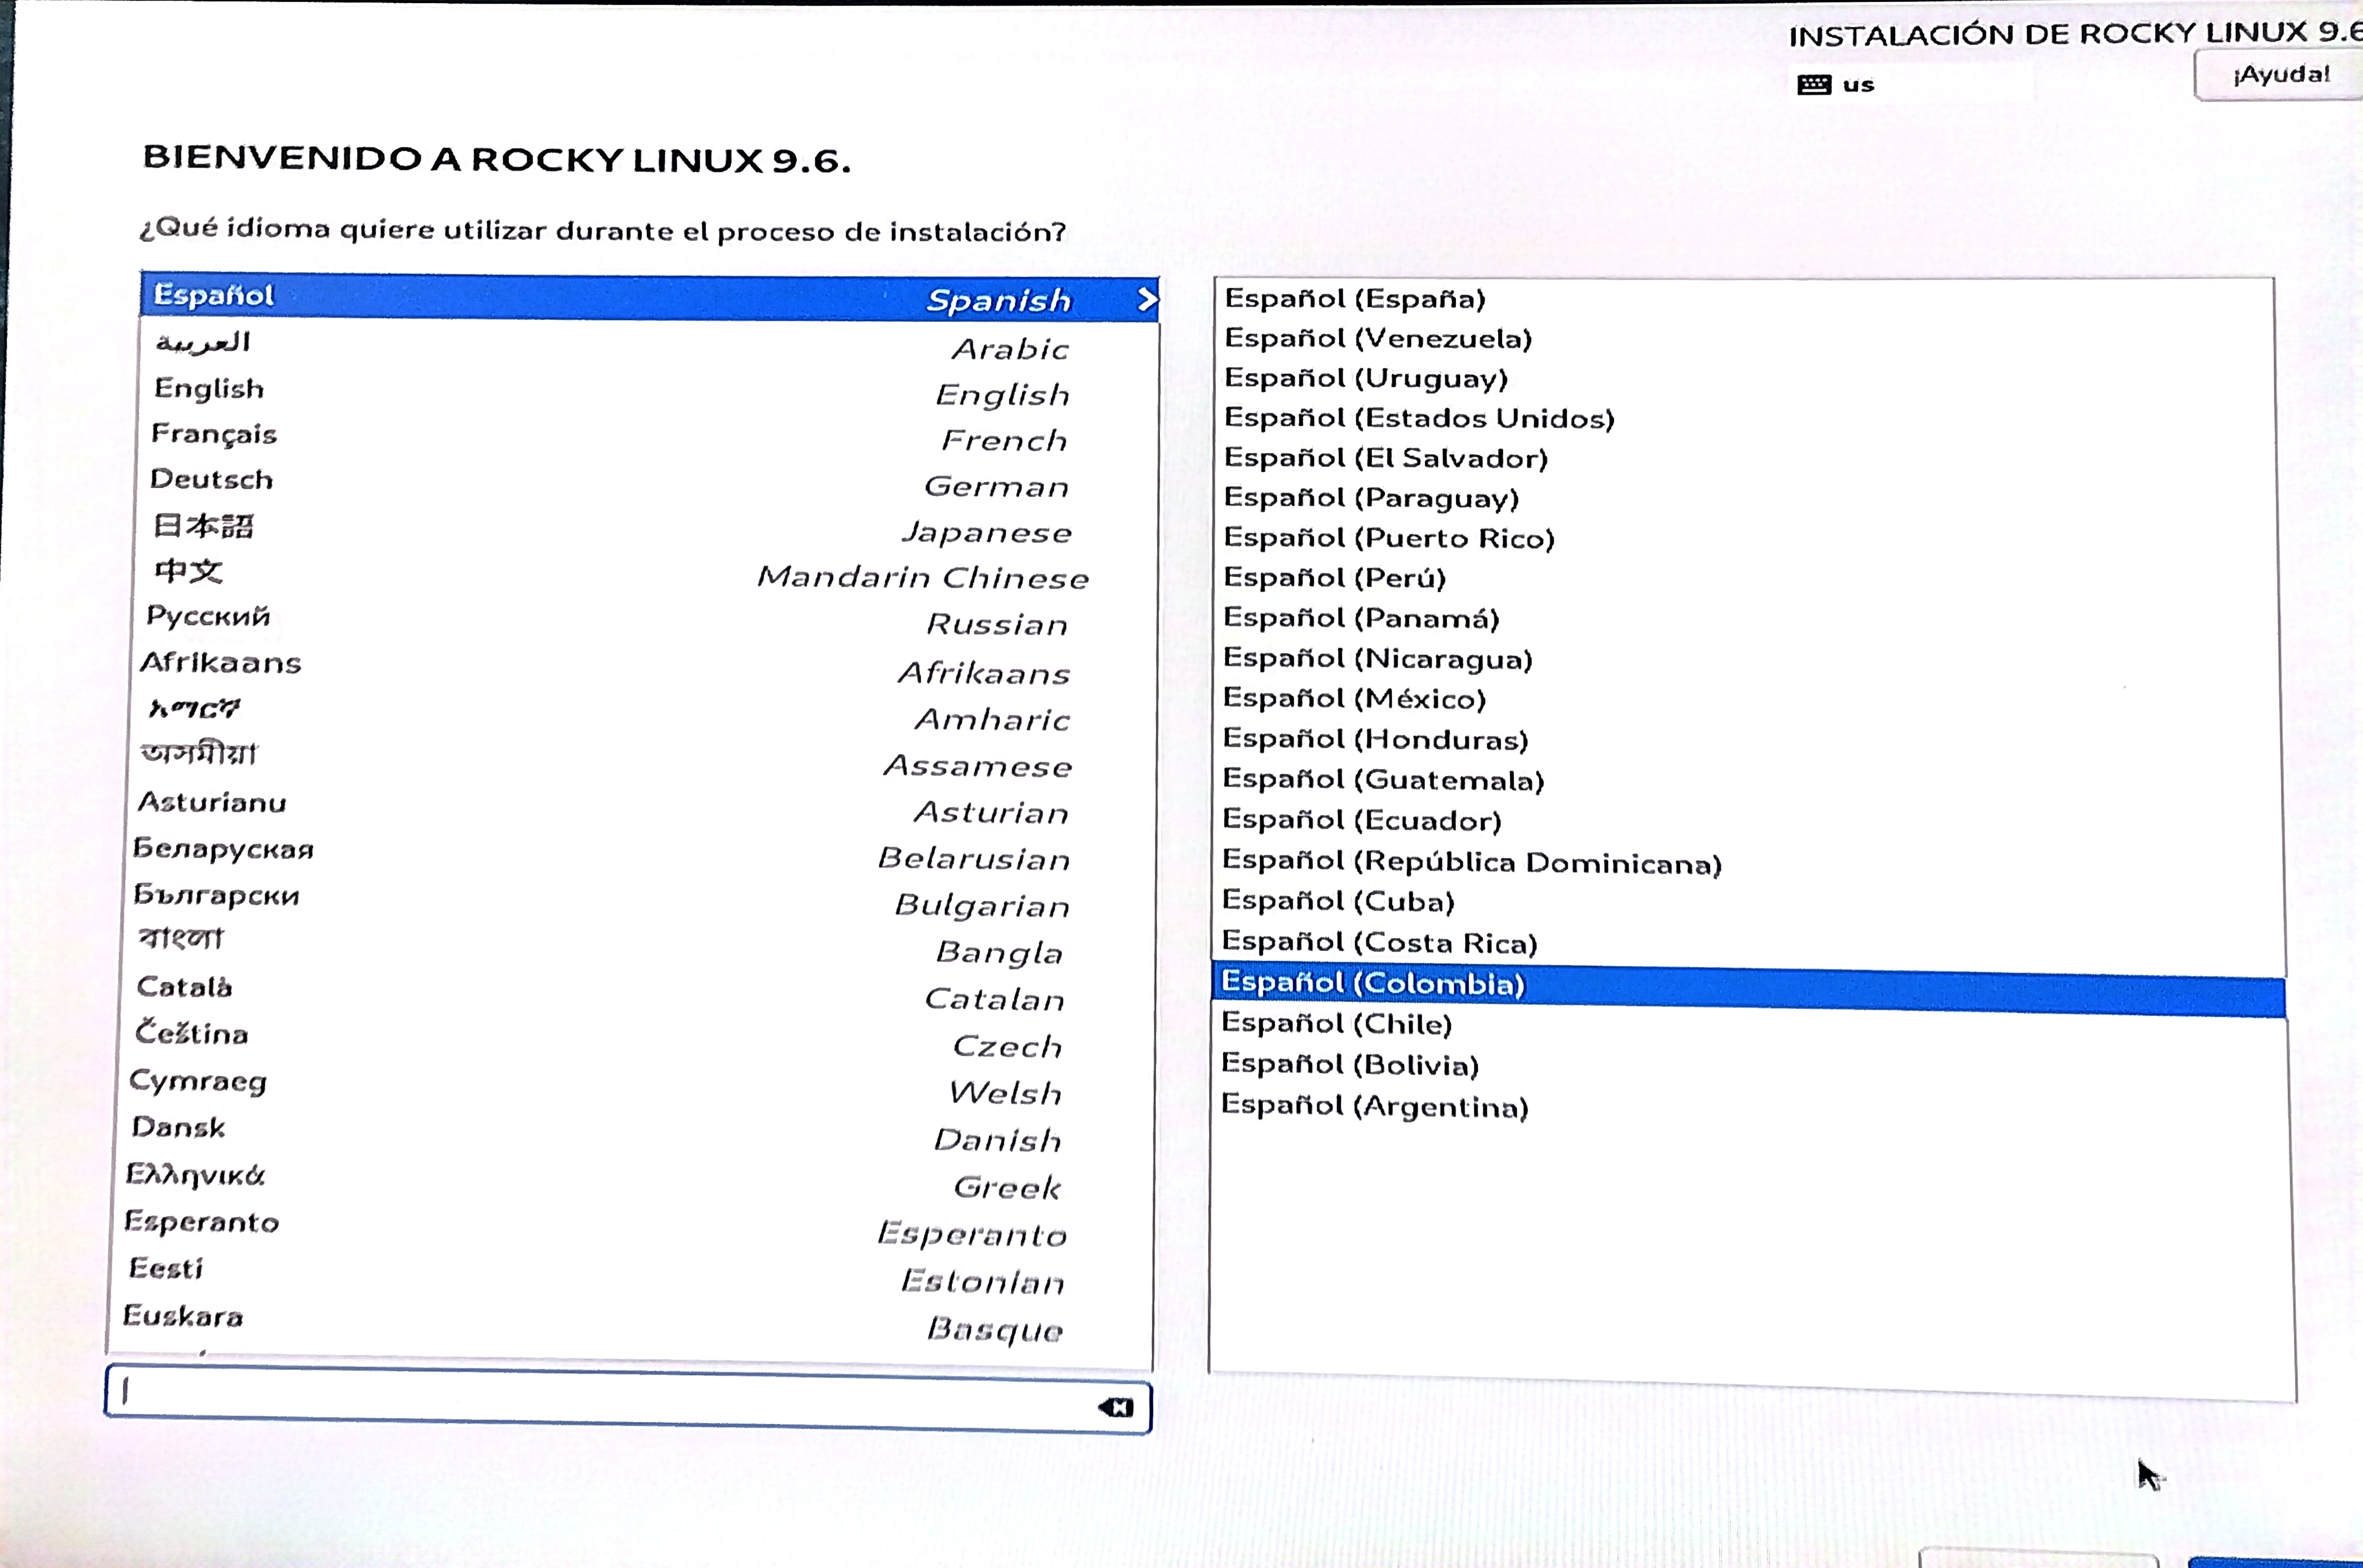
\includegraphics[width=0.92\textwidth]{images/HPC/SO/language_spanish.jpg}
  \caption{Selección de idioma del instalador.}
  \label{fig:language_spanish}
\end{figure}

En la pantalla \textit{Resumen de instalación}, se configuraron los bloques principales. \cite{rocky_install_9_6}

\begin{figure}[H]
  \centering
  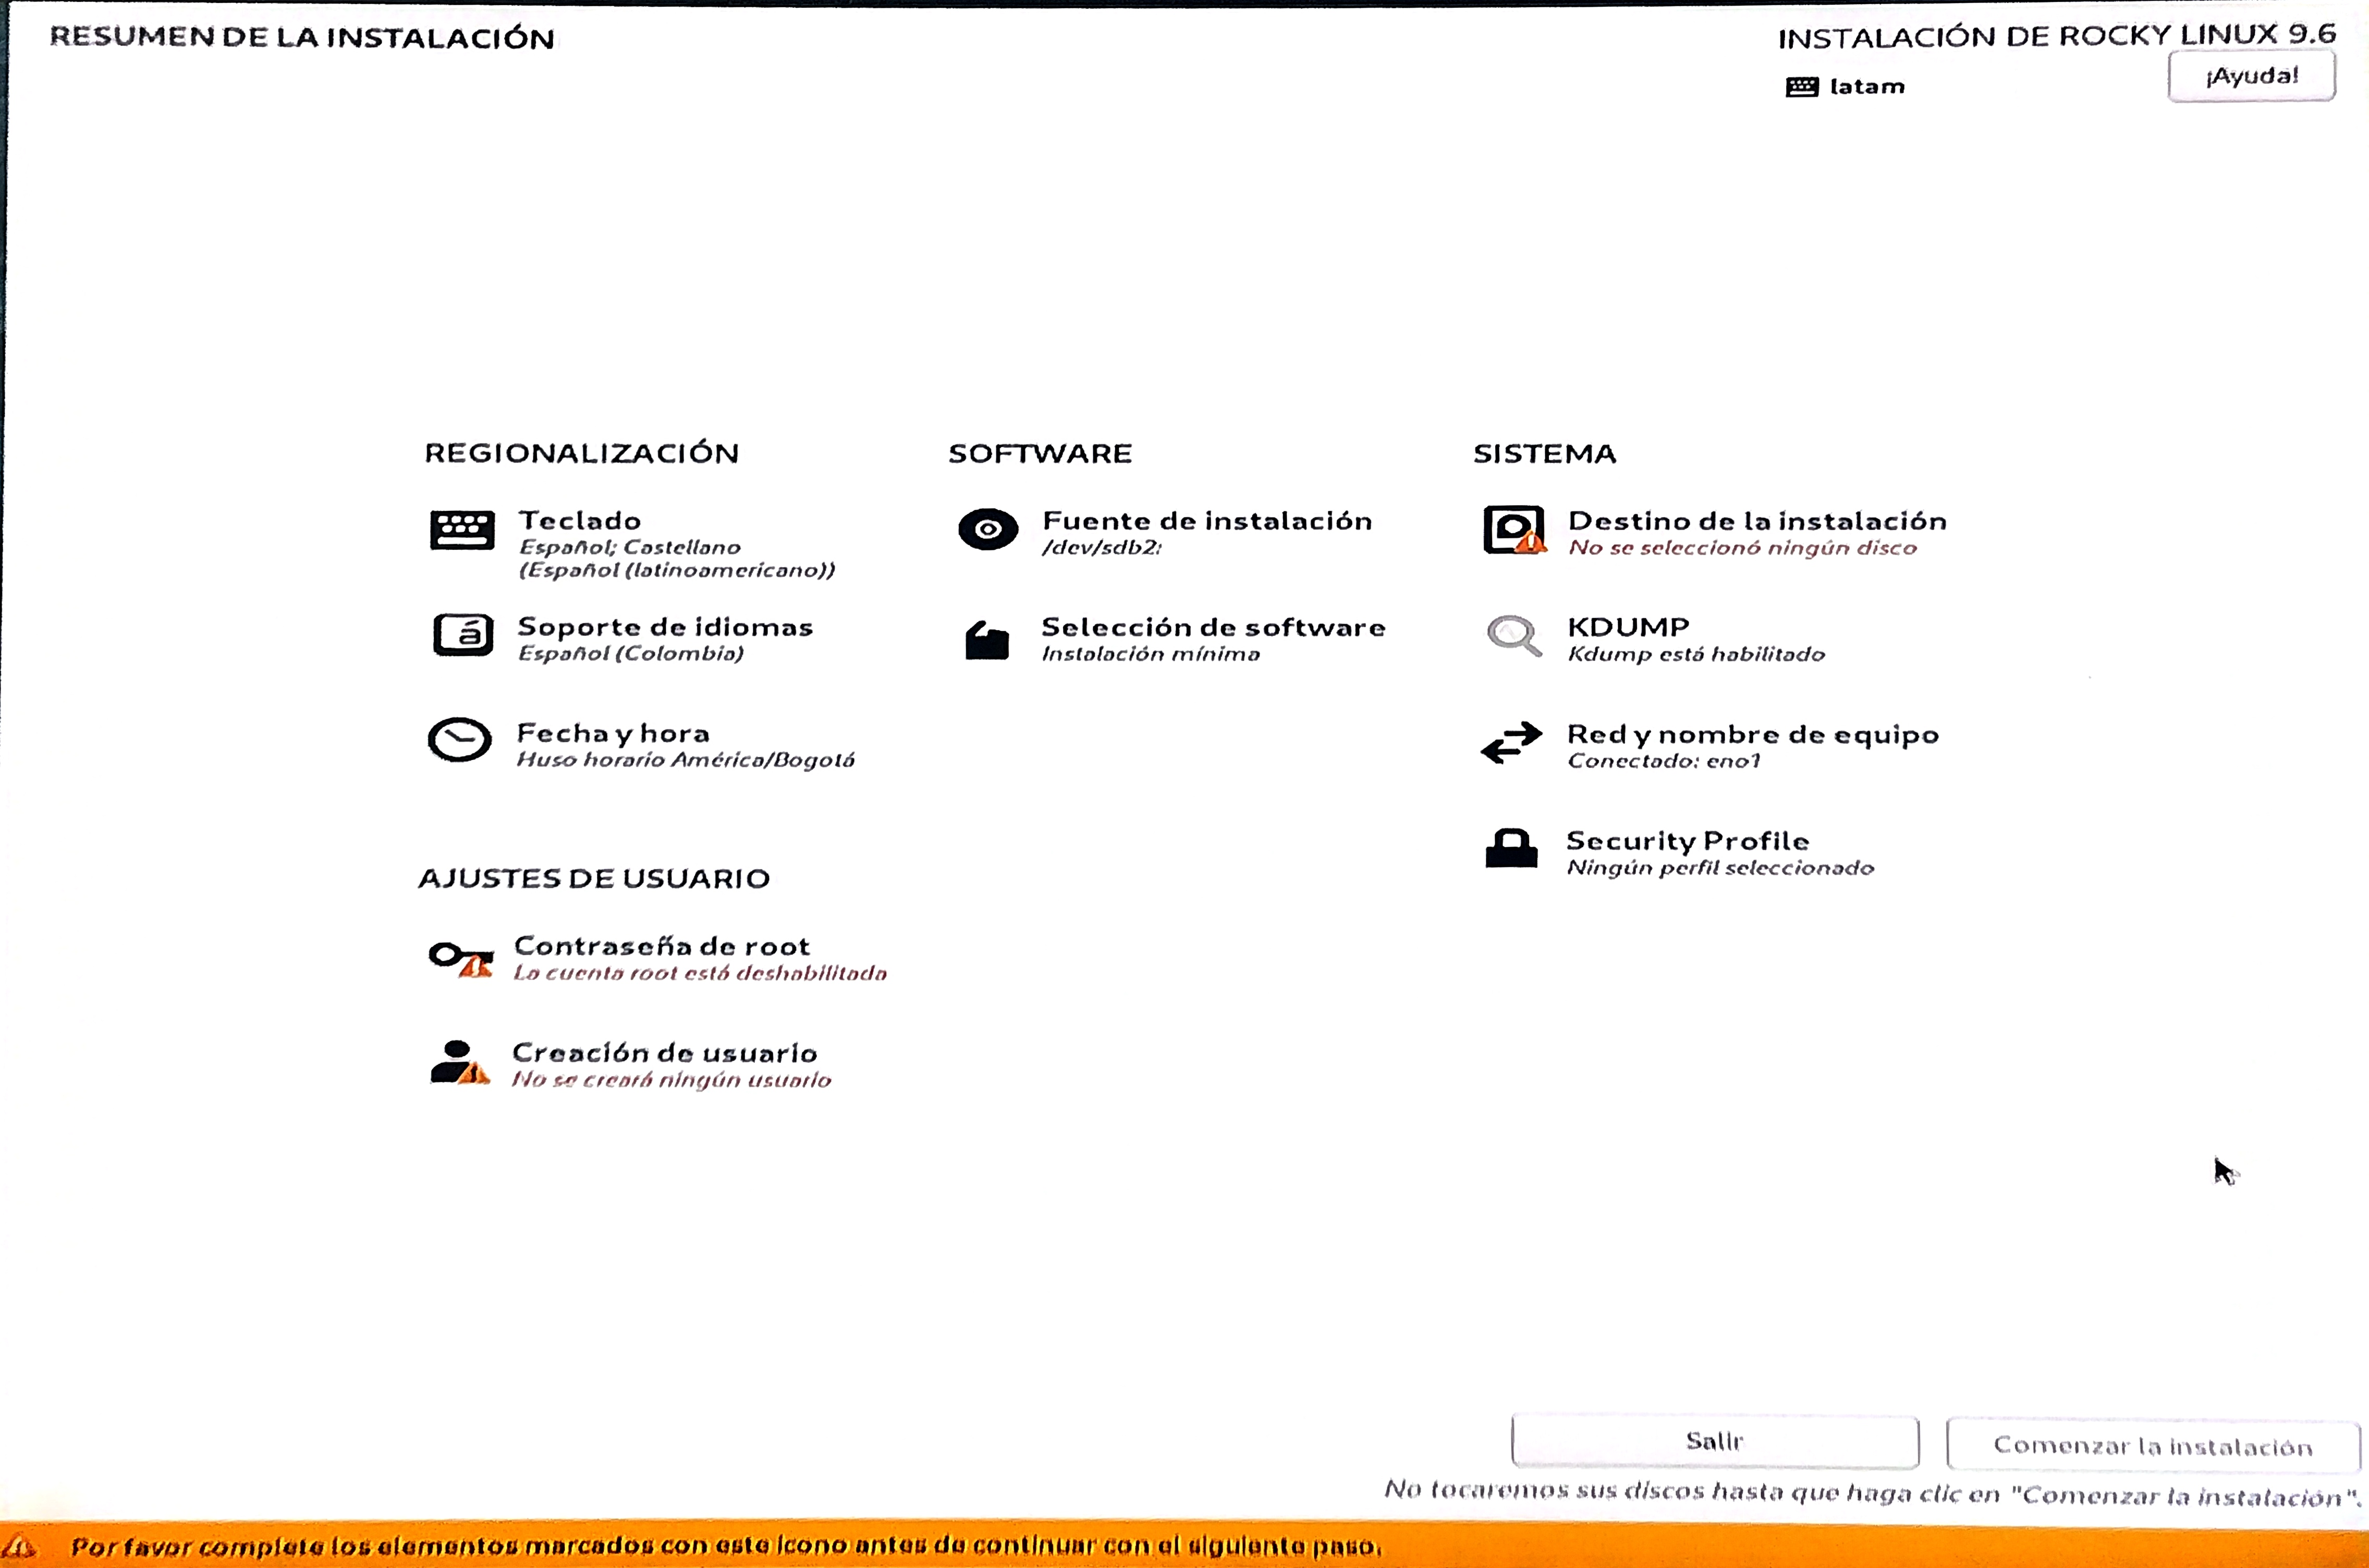
\includegraphics[width=0.92\textwidth]{images/HPC/SO/Resumen de instalación.jpg}
  \caption{Pantalla \textit{Resumen de instalación} del instalador de Rocky Linux.}
  \label{fig:installation_summary}
\end{figure}

\begin{enumerate}
  \setcounter{enumi}{1}
  \item En \textbf{Keyboard}, se seleccionó \textit{Spanish (Latin American)} (o equivalente).
\end{enumerate}

\begin{enumerate}
  \setcounter{enumi}{2}
  \item En \textbf{Time \& Date}, se configuró la zona horaria \textit{America/Bogota}.
\end{enumerate}

% \begin{figure}[H]
%   \centering
%   \includegraphics[width=0.92\textwidth]{images/configuración_del_entorno/07_time_date_bogota.png}
%   \caption{Zona horaria configurada (America/Bogota).}
%   \label{fig:time_date_bogota}
% \end{figure}

Al regresar al resumen, se verificó visualmente que estos apartados quedaron sin advertencias.

\subsubsection*{Selección de software base durante la instalación (Minimal Install)}
Durante la instalación del \textit{master} se eligió \textbf{Minimal Install} para dejar una base ligera y controlada, evitando componentes no necesarios en una primera fase. Esta decisión facilita el mantenimiento y reduce el número de paquetes instalados inicialmente. \cite{rocky_install_9_6}

\begin{enumerate}
  \item En \textbf{Software Selection}, se seleccionó \textbf{Minimal Install}.
  \item Se guardó la selección y se volvió a \textit{Resumen de instalación}. \cite{rocky_install_9_6}
\end{enumerate}

\begin{figure}[H]
  \centering
  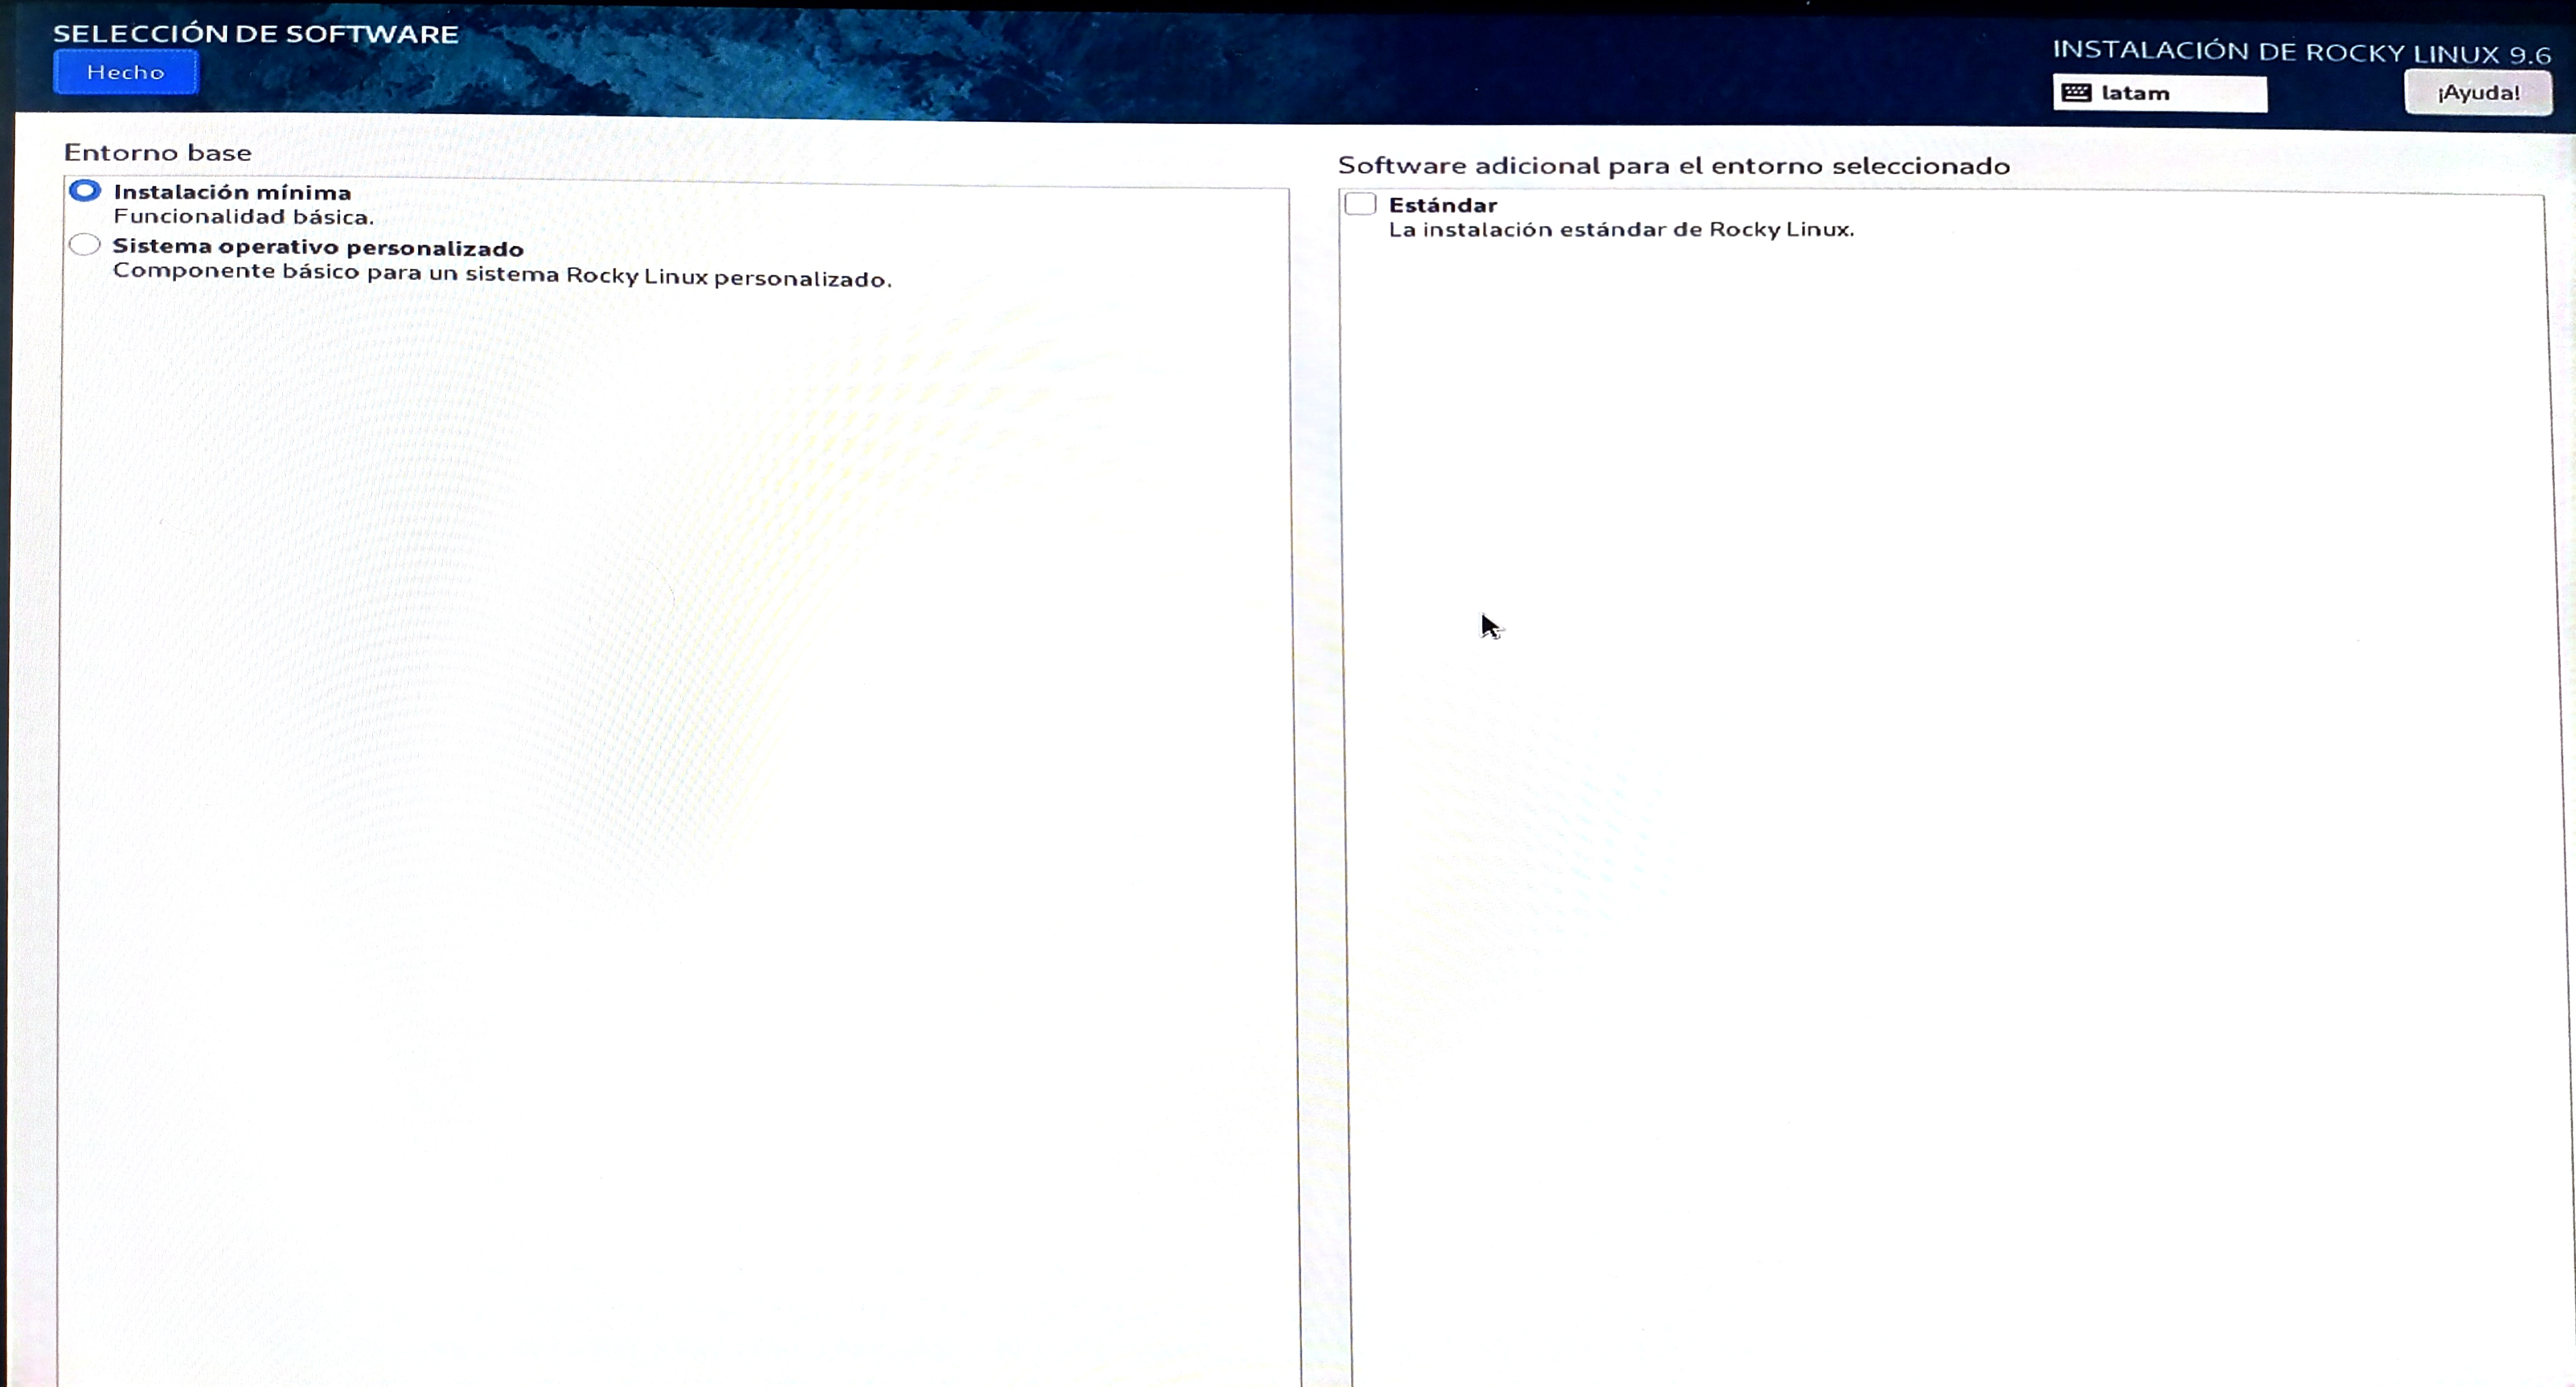
\includegraphics[width=0.92\textwidth]{images/HPC/SO/inst_minimal.jpg}
  \caption{Selección de software base: Minimal Install.}
  \label{fig:software_minimal}
\end{figure}

\subsubsection*{Selección de discos y particionado manual (Custom)}
El clúster separa el sistema operativo del almacenamiento de trabajo. El sistema se instaló en el NVMe para mejorar tiempos de arranque y respuesta, mientras que los volúmenes grandes en disco SATA se reservaron para datos y área de trabajo temporal (\textit{scratch}). La separación ayuda a mantener estable el sistema aunque crezcan los datos del proyecto.

\begin{enumerate}
  \item En \textbf{Installation Destination}, se seleccionó el disco \texttt{nvme0n1} como destino principal del sistema operativo.
  \item Se eligió configuración de almacenamiento \textbf{Custom} (particionado manual).
  \item Se definió el esquema de particiones exactamente como se muestra a continuación y se aplicaron los cambios.
\end{enumerate}

% \begin{figure}[H]
%   \centering
%   \includegraphics[width=0.92\textwidth]{images/configuración_del_entorno/09_installation_destination.png}
%   \caption{Selección de disco y entrada al particionado manual (Custom).}
%   \label{fig:installation_destination}
% \end{figure}

% \begin{figure}[H]
%   \centering
%   \includegraphics[width=0.92\textwidth]{images/configuración_del_entorno/10_custom_partitioning.png}
%   \caption{Pantalla de particionado manual (Custom) en el instalador.}
%   \label{fig:custom_partitioning}
% \end{figure}

\begin{table}[H]
\centering
\caption{Esquema de particiones aplicado durante la instalación del nodo master.}
\label{tab:particiones_master}
\begin{tabular}{llll}
\hline
\textbf{Disco} & \textbf{Punto de montaje} & \textbf{Tamaño} & \textbf{Sistema} \\
\hline
\texttt{nvme0n1} & \texttt{/boot/efi} & 300 MiB & EFI \\
\texttt{nvme0n1} & \texttt{/boot} & 1 GiB & XFS \\
\texttt{nvme0n1} & \texttt{/} & 80 GiB & XFS \\
\texttt{nvme0n1} & \texttt{/var} & 40 GiB & XFS \\
\texttt{nvme0n1} & \texttt{/opt} & 60 GiB & XFS \\
\texttt{nvme0n1} & \texttt{/home} & 30 GiB & XFS \\
\texttt{nvme0n1} & \texttt{swap} & 8 GiB & swap \\
\texttt{sda} & \texttt{/data} & 2000 GiB & XFS \\
\texttt{sda} & \texttt{/scratch} & 2000 GiB & XFS \\
\hline
\end{tabular}
\end{table}

En el proceso, \texttt{/var} se separó para aislar registros y cachés del sistema, \texttt{/opt} para software adicional instalado fuera del sistema base, y \texttt{/scratch} como espacio de trabajo temporal (útil para ejecuciones intermedias o archivos transitorios). Tras aplicar el esquema, el instalador permitió continuar sin alertas críticas, lo cual confirmó que los montajes y tamaños eran válidos.

\subsubsection*{Red y nombre del equipo (Network \& Hostname)}
La red se activa durante la instalación para que el nodo quede accesible y se pueda administrar posteriormente.

\begin{enumerate}
  \item En \textbf{Network \& Hostname}, se activó la interfaz de red principal.
  \item Se asignó el nombre del host como \texttt{master}.
  \item Se observó en pantalla la dirección IP entregada por DHCP para referencia durante la instalación. \cite{rocky_install_9_6}
\end{enumerate}

\begin{figure}[H]
  \centering
  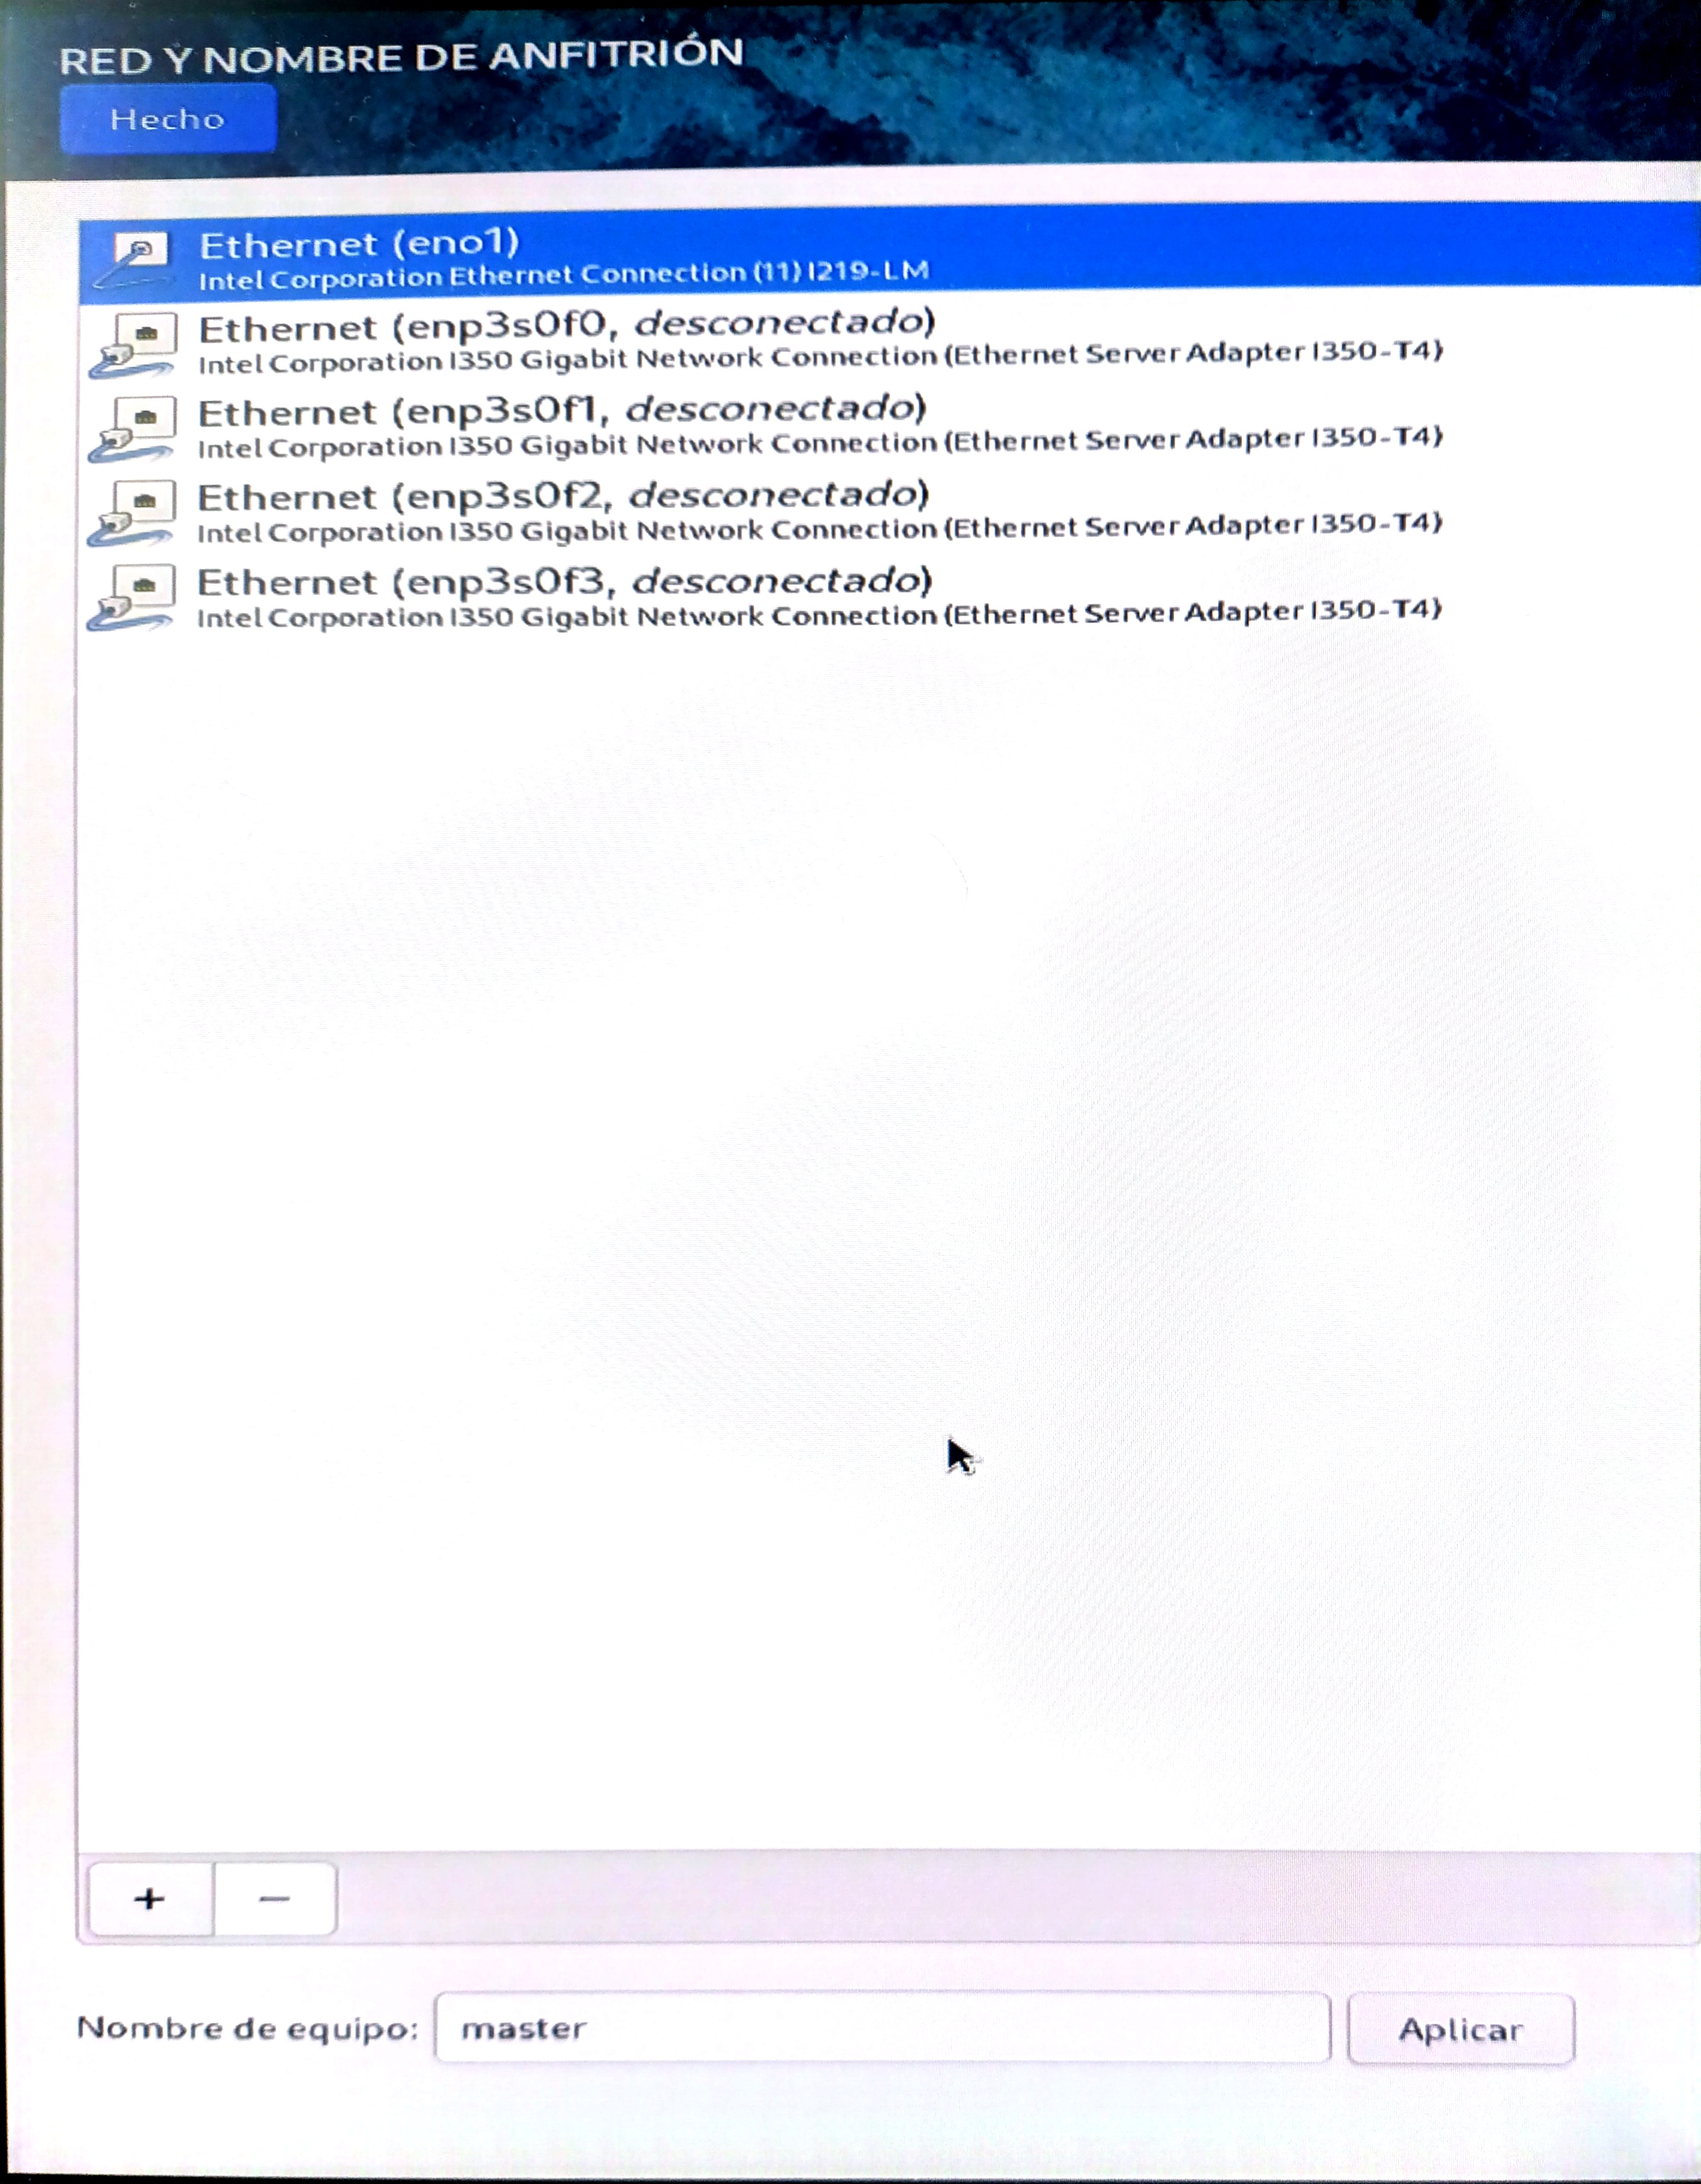
\includegraphics[width=0.9\textwidth]{images/HPC/SO/red_hostname.jpg}
  \caption{Red activada y hostname configurado como \texttt{master}.}
  \label{fig:network_hostname_master}
\end{figure}

\subsubsection*{Credenciales iniciales e instalación}
\begin{enumerate}
  \item Se configuró la contraseña de \texttt{root} como \texttt{sistemas}.

  \begin{figure}[H]
    \centering
    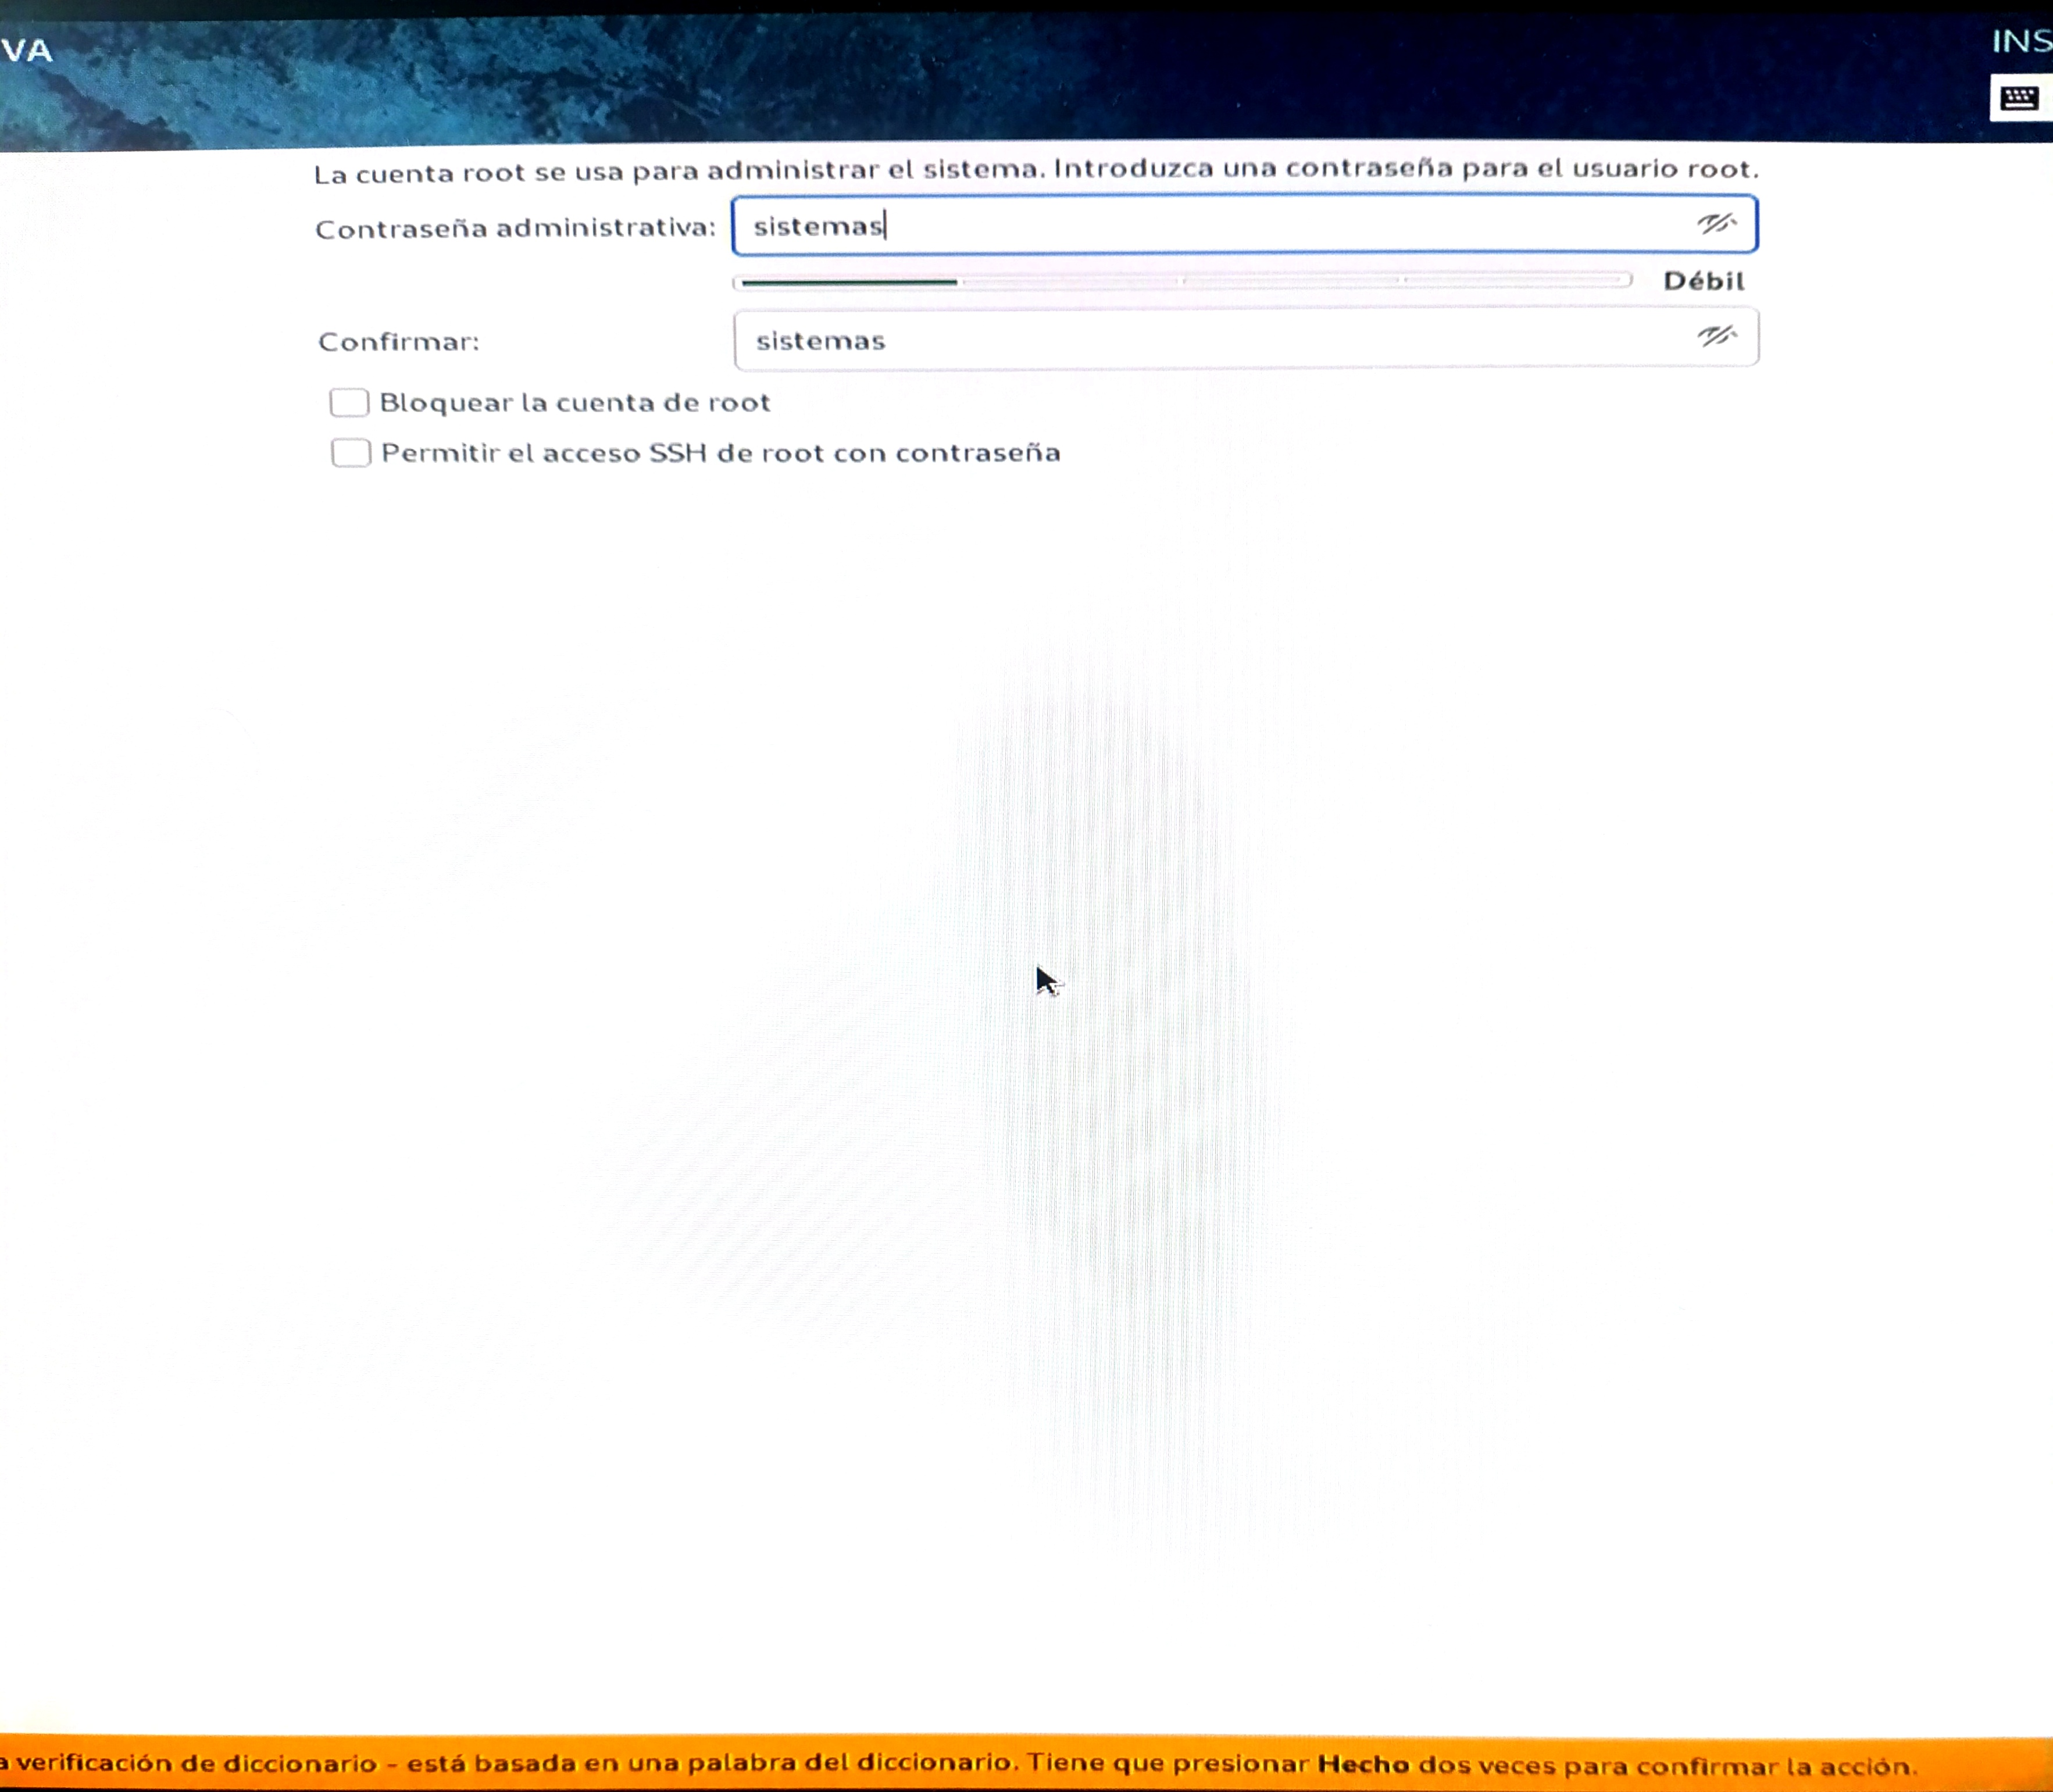
\includegraphics[width=0.92\textwidth] {images/HPC/SO/passwd_root.jpg}
    \caption{Pantalla de configuración de contraseña de root.}
    \label{fig:root_password}
  \end{figure}

  \item Se creó el usuario administrativo \texttt{sistemas} con permisos para tareas administrativas.

  \begin{figure}[H]
    \centering
    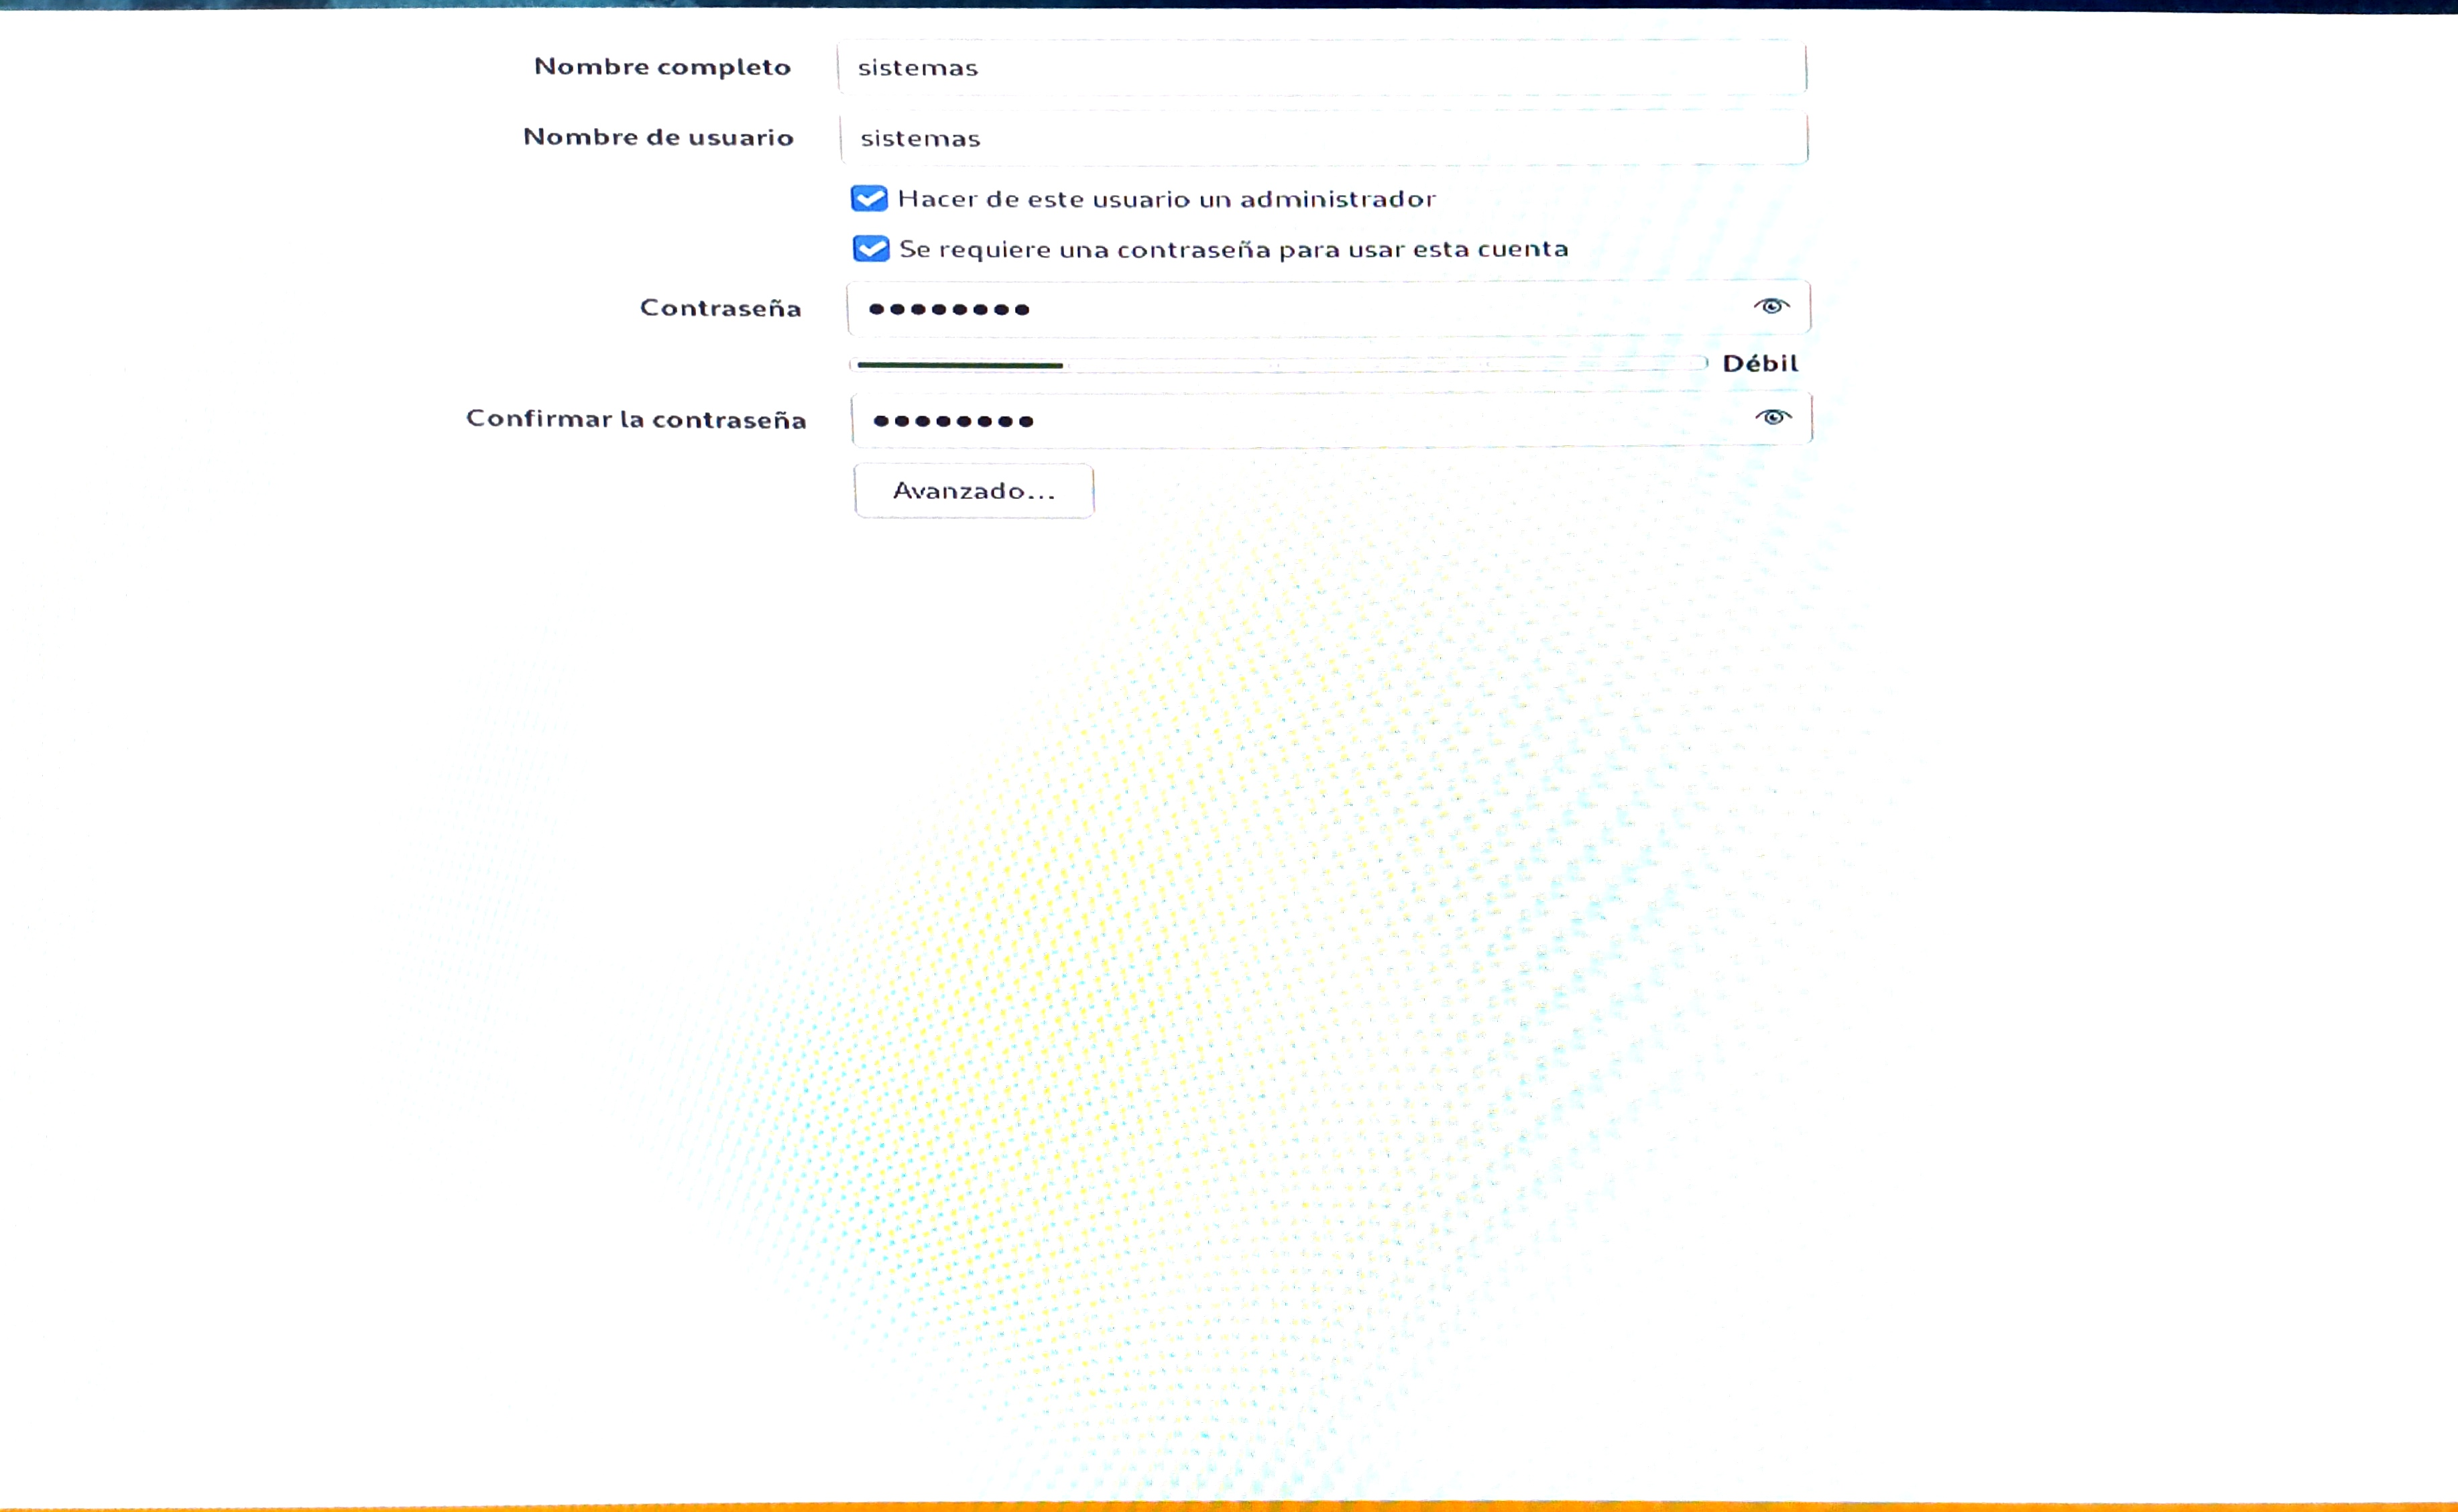
\includegraphics[width=0.92\textwidth]{images/HPC/SO/usr_sistemas.jpg}
    \caption{Creación del usuario \texttt{sistemas} (sin exponer contraseñas).}
    \label{fig:user_creation}
  \end{figure}

  
\end{enumerate}

\subsubsection{Inicio de la instalación}
\begin{enumerate}
  \item En la pantalla \texttt{Resumen de instalación} se verifica que todos los componentesno muestren mensajes de error y/o alertas.
  \item Se inició la instalación desde \textit{Comenzar instalación}.
\end{enumerate}

\begin{figure}[H]
  \centering
  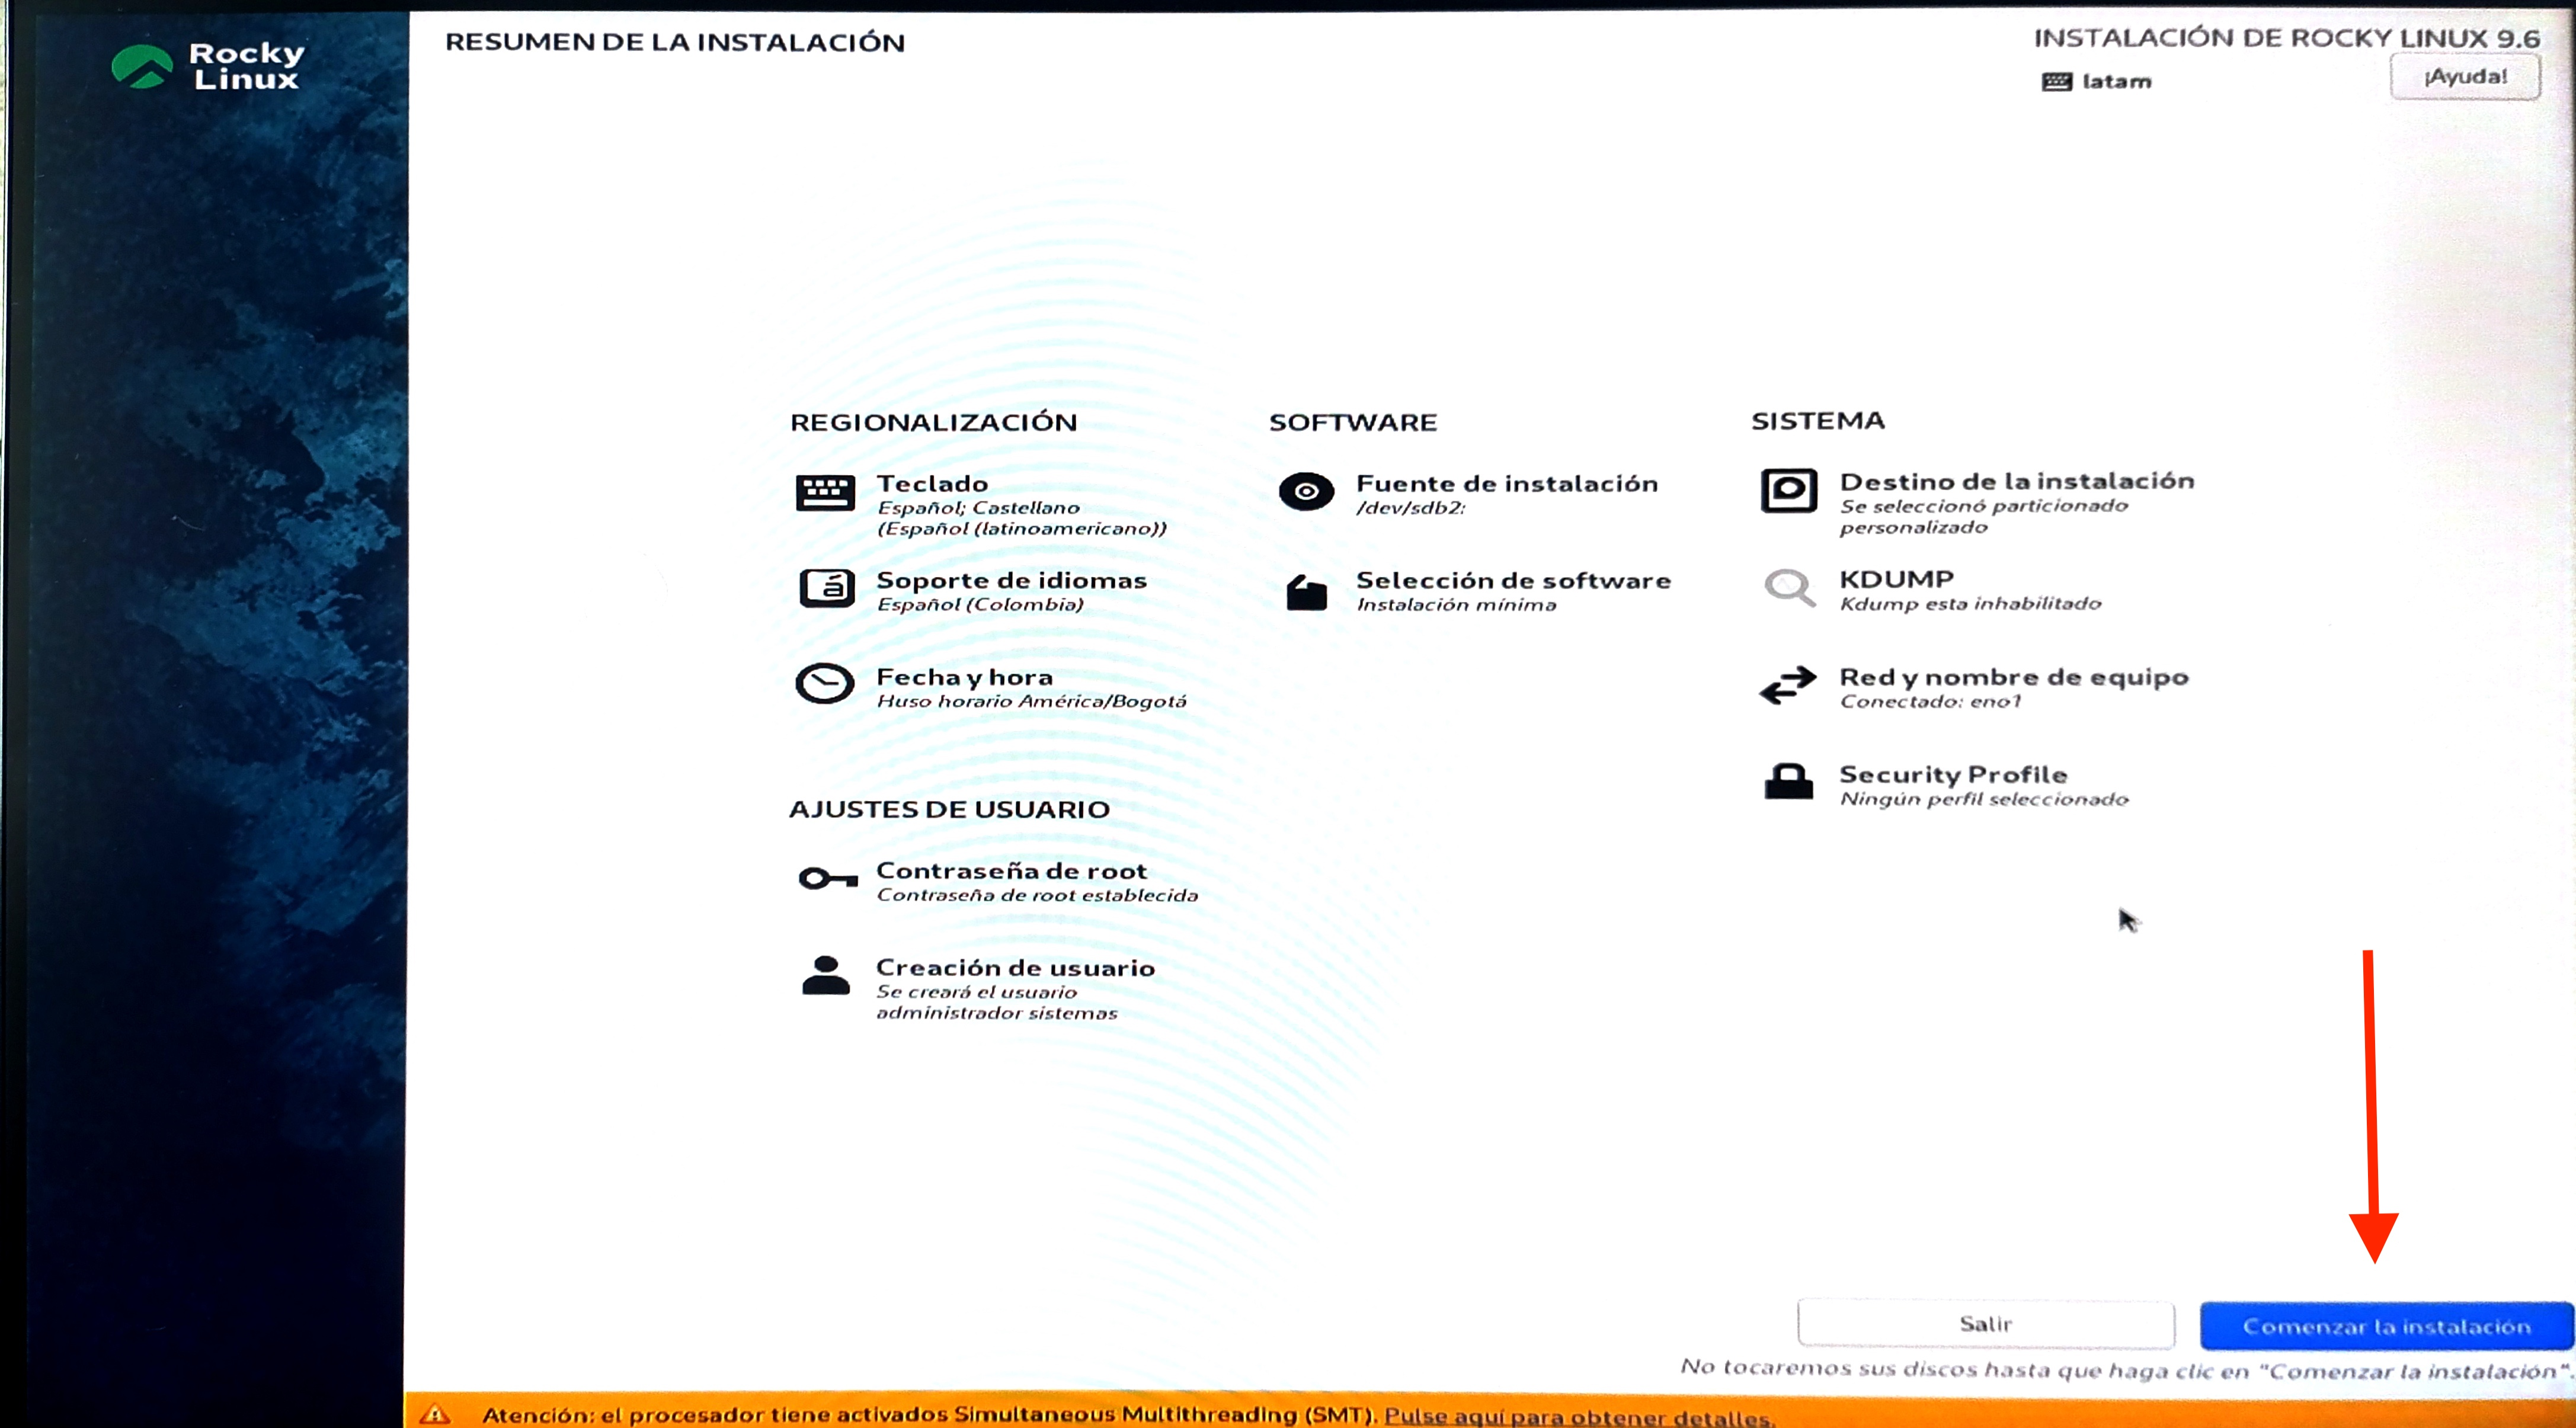
\includegraphics[width=0.92\textwidth]{images/HPC/SO/resumen_inst_final.jpg}
  \caption{Estado de la pantalla \texttt{Resumen de instalación} al finalizar la configuración.}
  \label{fig:begin_installation}
\end{figure}



Al finalizar, el instalador mostró el mensaje de instalación completada y se reinició el sistema. Esto confirmó que el sistema operativo quedó instalado en el disco interno. \cite{rocky_install_9_6}

% \begin{figure}[H]
%   \centering
%   \includegraphics[width=0.92\textwidth]{images/configuración_del_entorno/14_install_complete.png}
%   \caption{Instalación completada y reinicio del sistema.}
%   \label{fig:install_complete}
% \end{figure}

\subsubsection*{Primer arranque y verificación inicial de particiones montadas}
En el primer arranque se confirma que el sistema inicia desde el disco y que las particiones se montan como se planearon.

\begin{enumerate}
  \item Se retiró la USB (o se evitó arrancar desde USB) para que el equipo iniciara desde el disco interno.
  \item Se inició sesión con el usuario \texttt{sistemas} y contraseña \texttt{sistemas}.

    \begin{figure}[H]
        \centering
        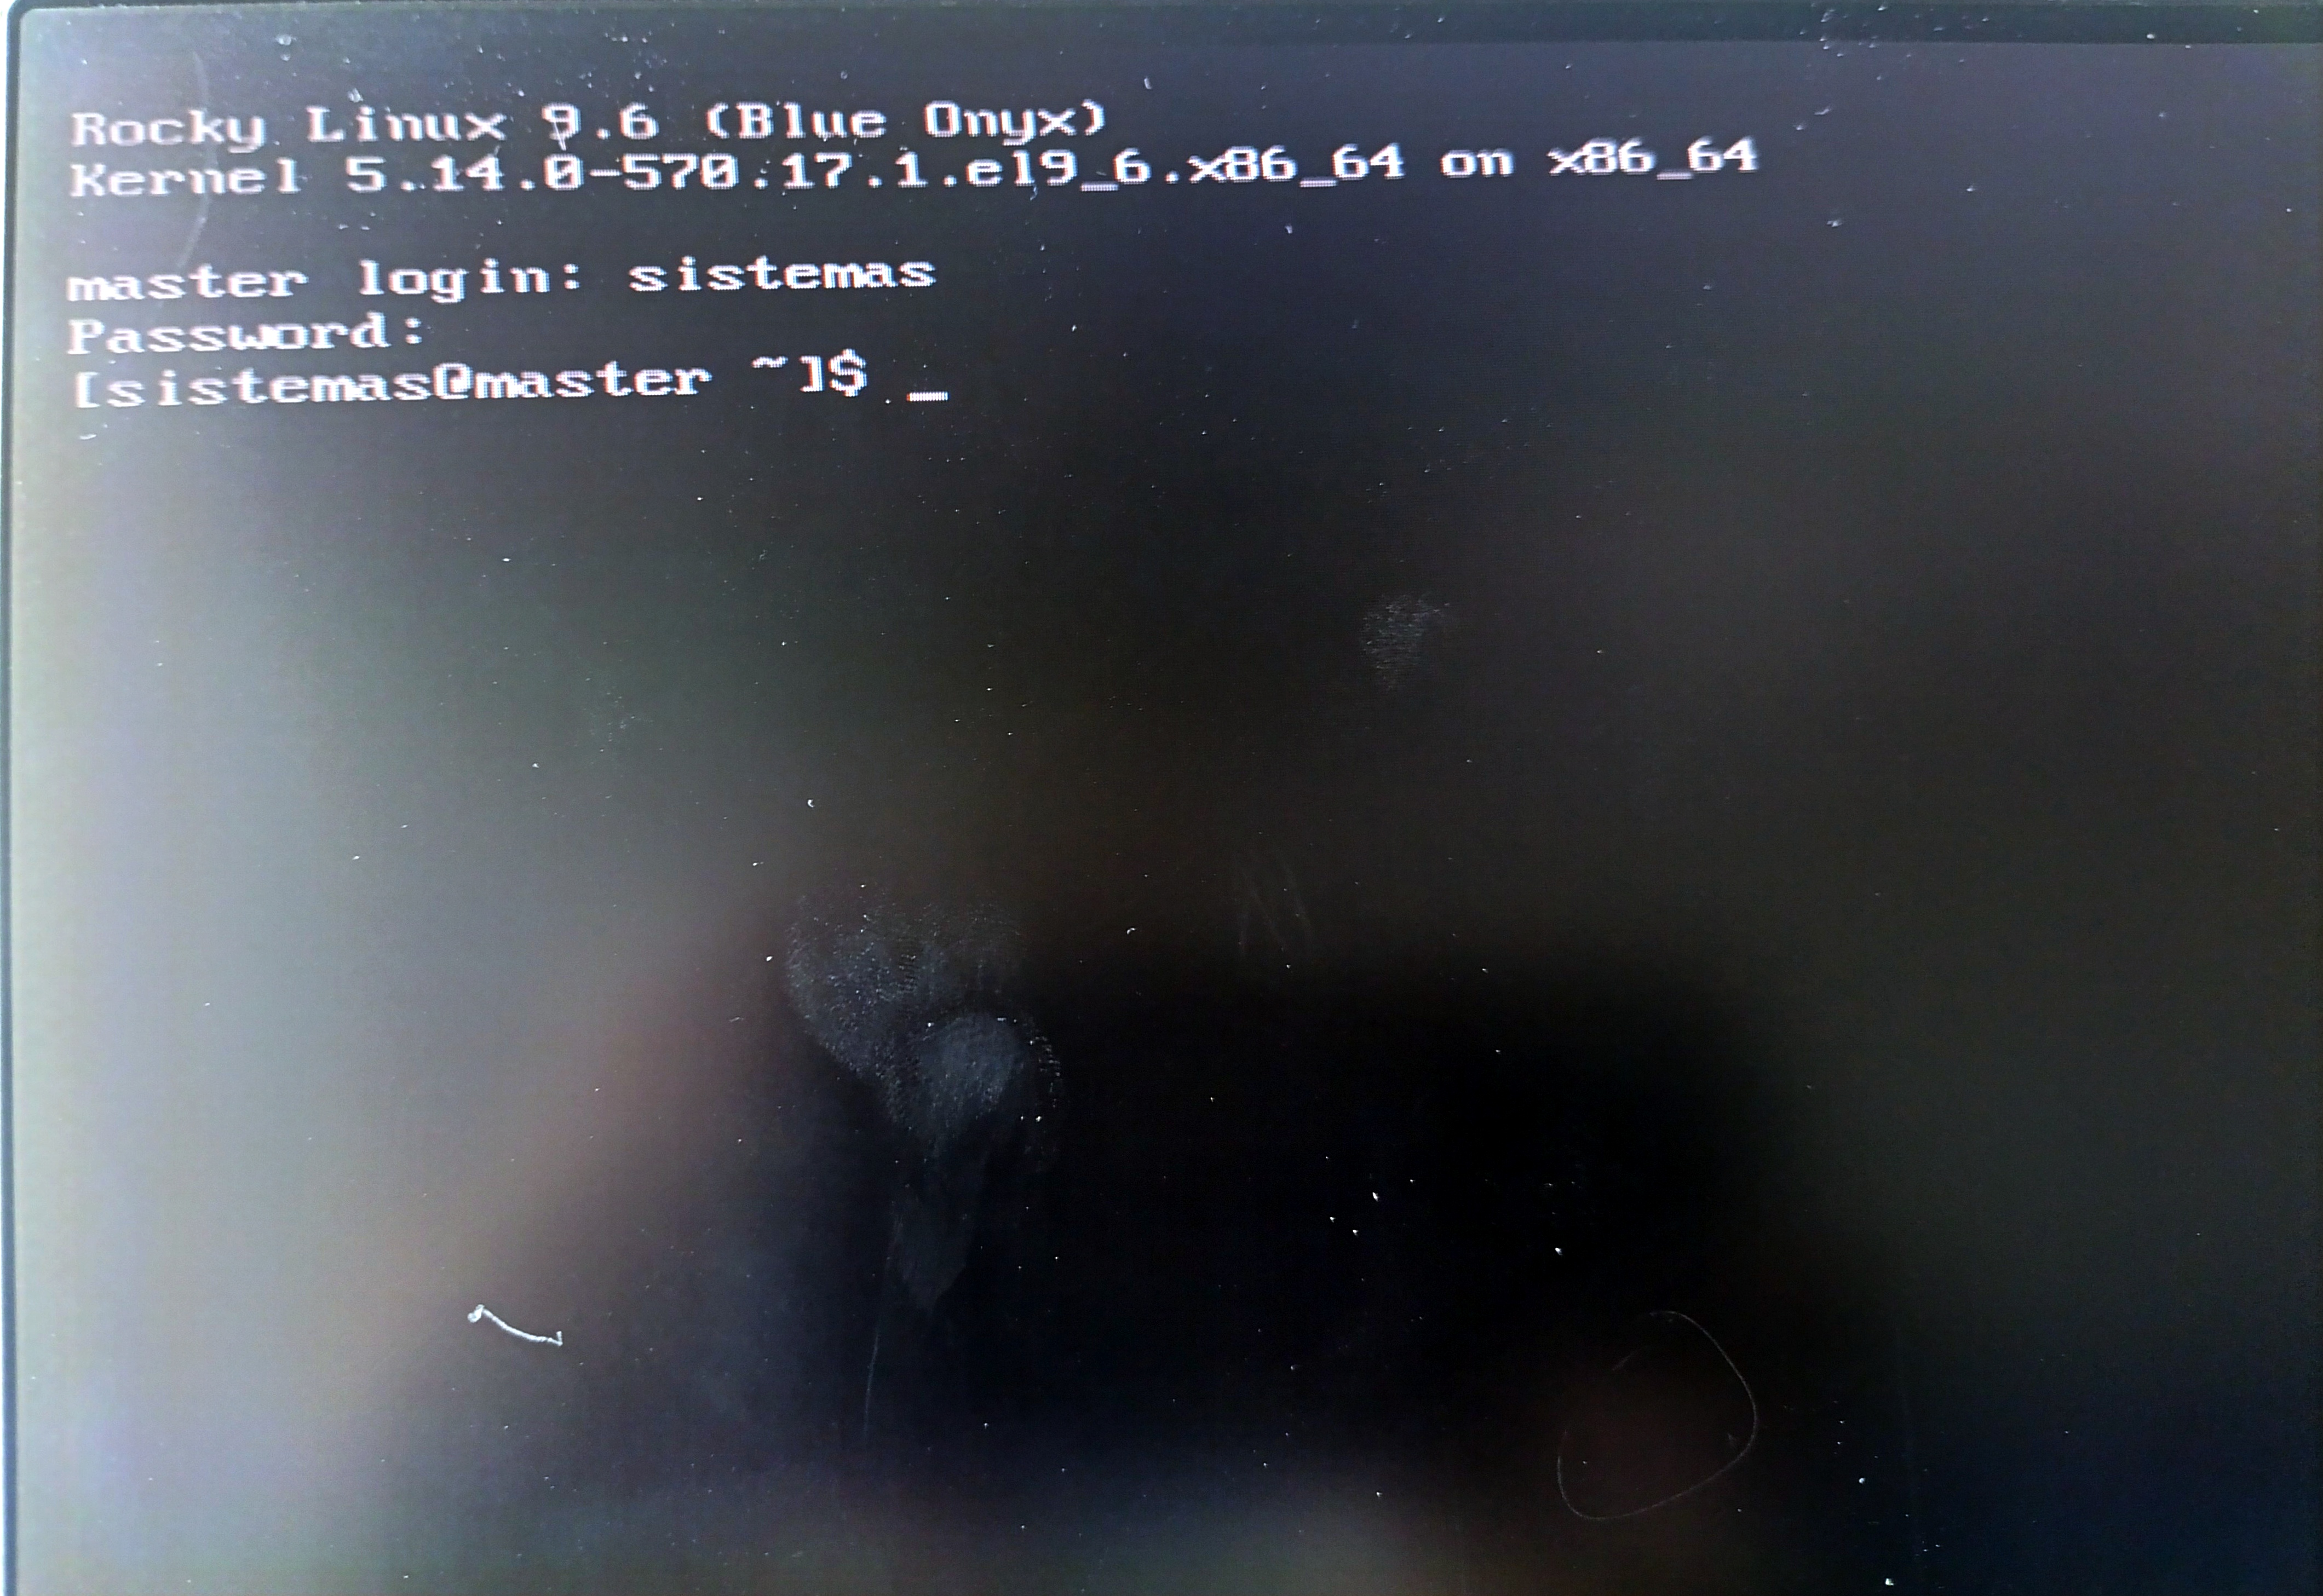
\includegraphics[width=0.5\linewidth]{images/HPC/Rocky/Rocky_start.jpg}
        \caption{Primera sesión en Rocky Linux (Minimal) }
        \label{fig:placeholder}
    \end{figure}
  
  \item Se ejecutaron los siguientes comandos para verificar discos, puntos de montaje y espacio disponible:
\end{enumerate}

\begin{verbatim}
lsblk
df -h
\end{verbatim}

\begin{figure}[H]
  \centering
  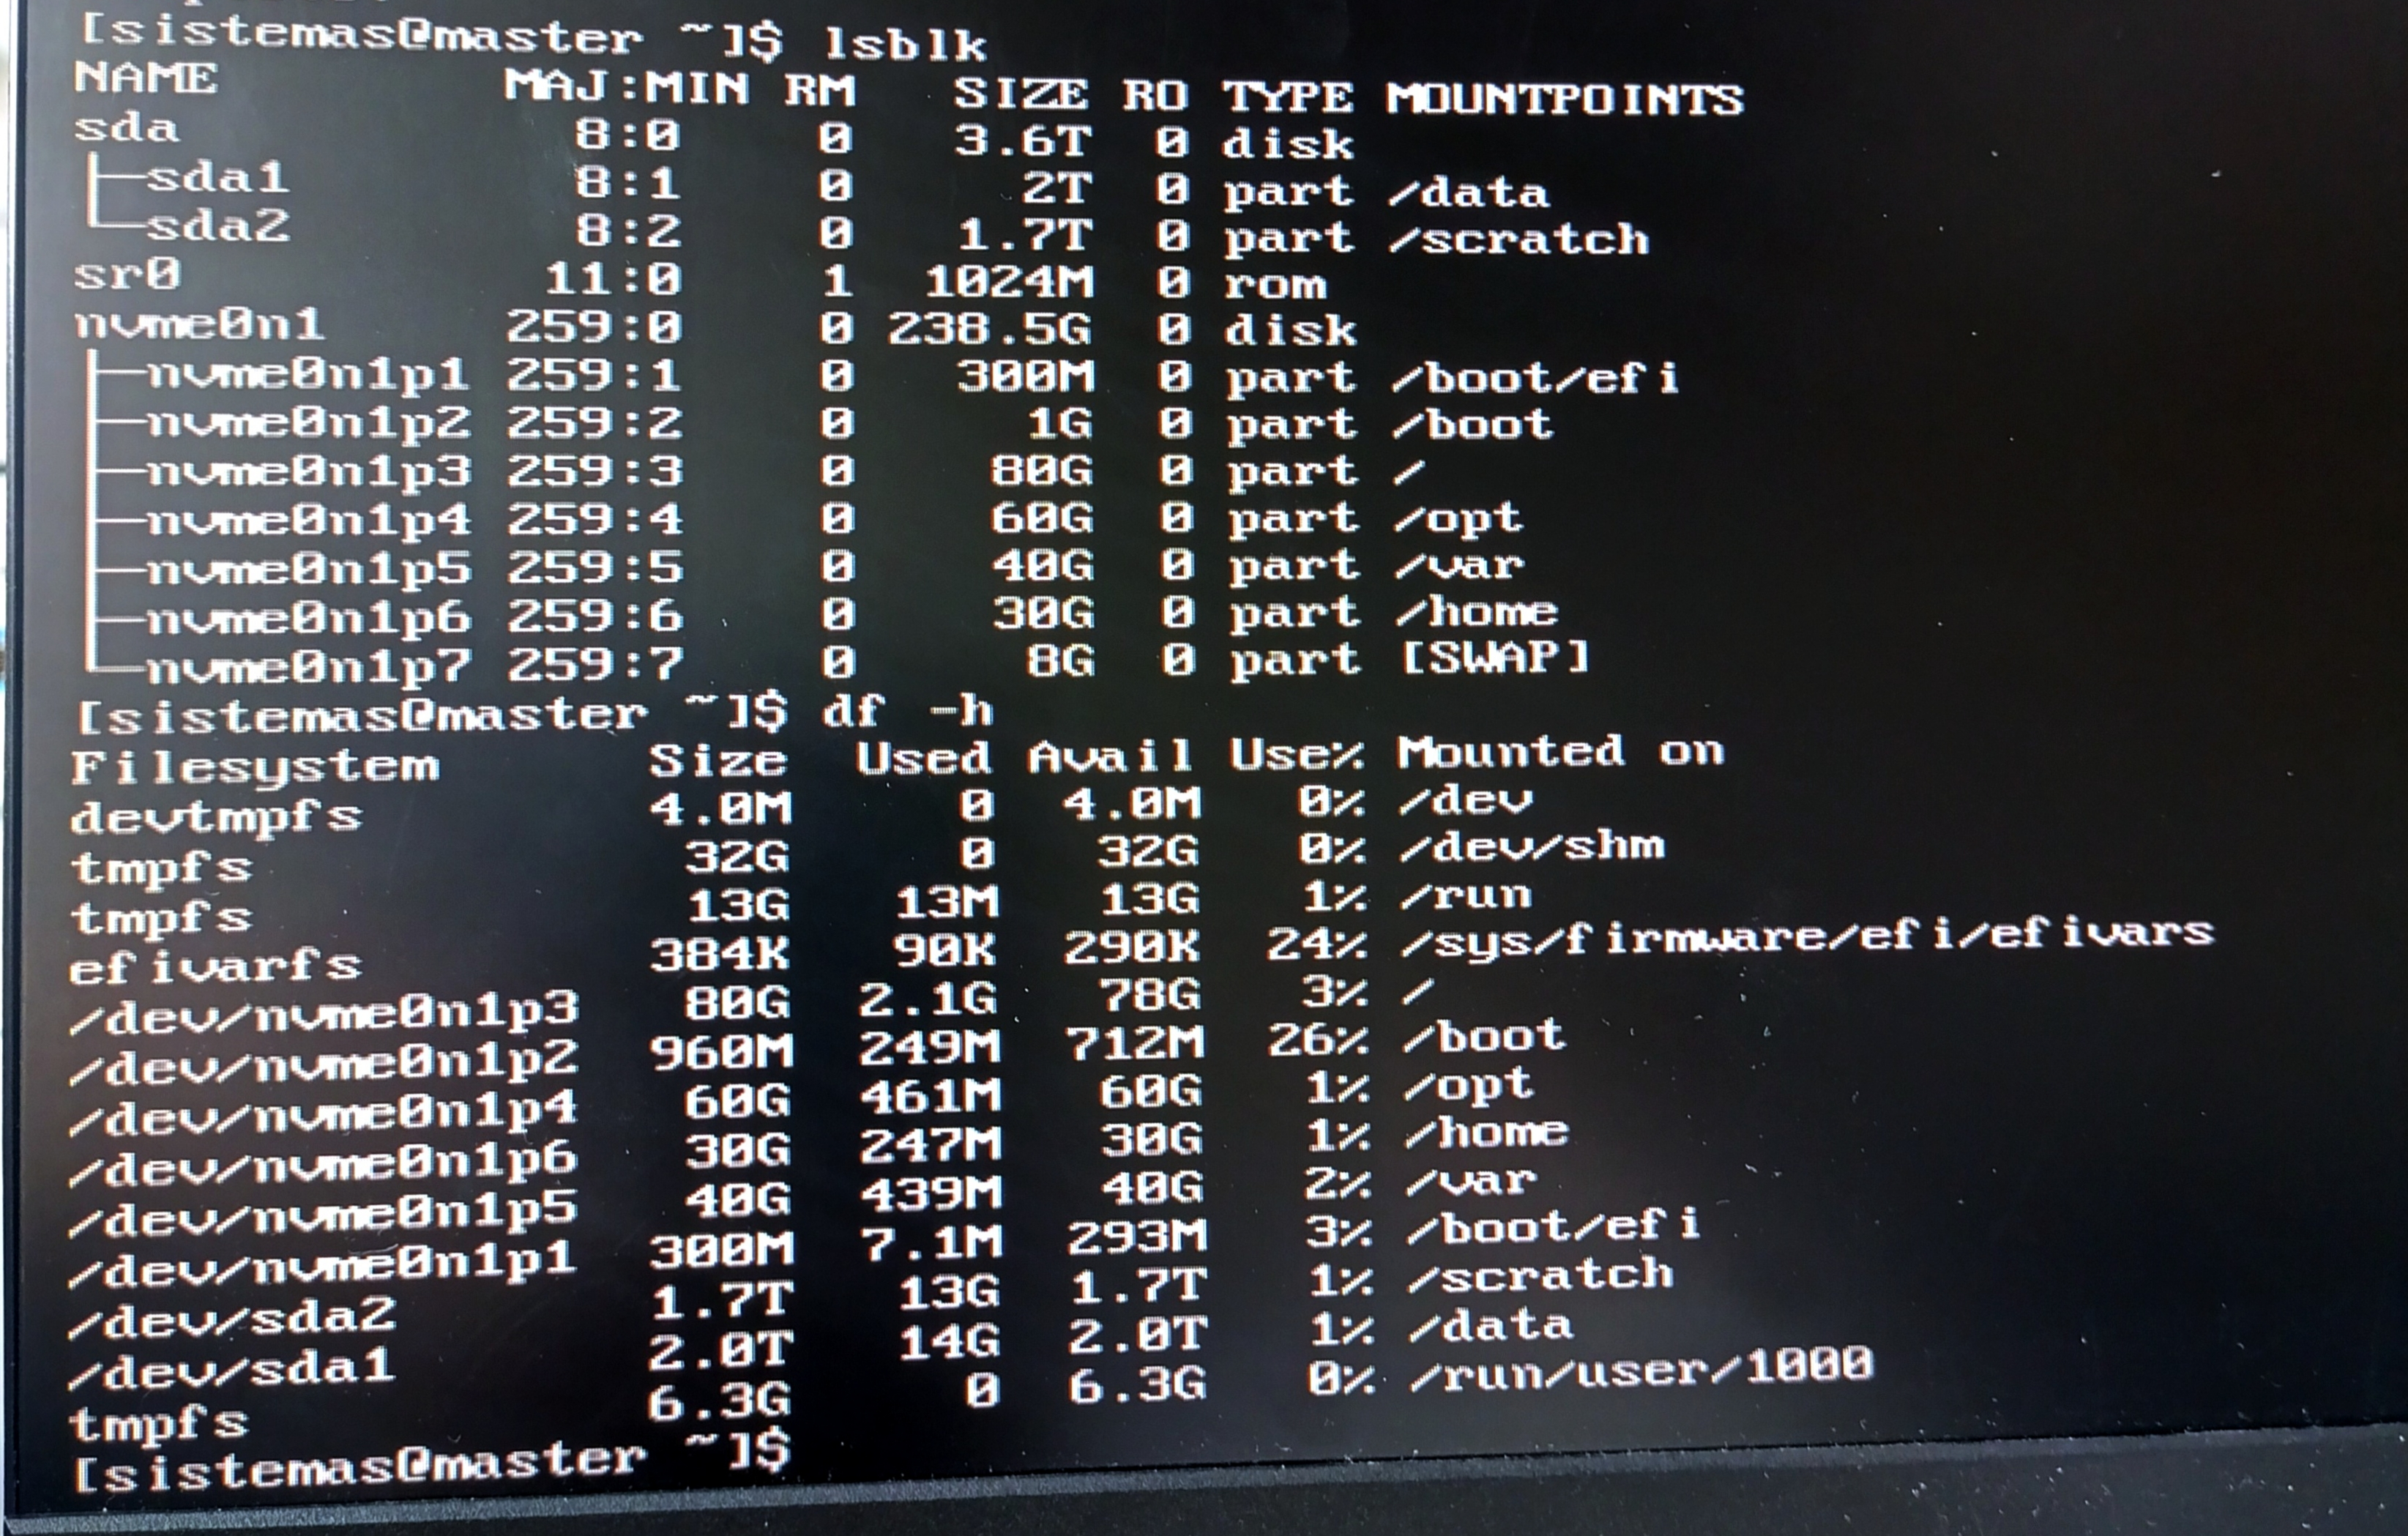
\includegraphics[width=0.5\textwidth]{images/HPC/Rocky/particiones.jpg}
  \caption{Verificación post-instalación: discos, puntos de montaje y espacio.}
  \label{fig:post_install_storage_check}
\end{figure}

Al revisar la salida, se observó que \texttt{/data} y \texttt{/scratch} estaban montados sobre \texttt{sda} y que las particiones del sistema (\texttt{/}, \texttt{/var}, \texttt{/opt}, \texttt{/home}) estaban montadas sobre \texttt{nvme0n1}, coherente con el esquema definido en el instalador.



\subsubsection*{Instalación posterior de interfaz gráfica en el master (Server with GUI)}
Aunque el nodo \textit{master} se instaló inicialmente como \textit{Minimal Install}, se agregó posteriormente un entorno gráfico para facilitar administración y tareas de configuración inicial. En Rocky Linux, el entorno \textit{Server with GUI} se instala como un grupo de paquetes mediante \texttt{dnf groupinstall}. \cite{rocky_forum_server_with_gui}

\begin{enumerate}
  \item Se actualizaron los repositorios y paquetes del sistema:
\end{enumerate}

\begin{verbatim}
sudo dnf -y update
\end{verbatim}

\begin{enumerate}
  \setcounter{enumi}{1}
  \item Se instaló el grupo \textit{Server with GUI}:
\end{enumerate}

\begin{verbatim}
sudo dnf groupinstall "Server with GUI"
\end{verbatim}

Tras completarse la instalación, se configuró el arranque por defecto en modo gráfico para que el entorno iniciara automáticamente.

\begin{verbatim}
sudo systemctl set-default graphical.target
sudo reboot
\end{verbatim}

% \begin{figure}[H]
%   \centering
%   \includegraphics[width=0.92\textwidth]{images/configuración_del_entorno/16_groupinstall_server_with_gui.png}
%   \caption{Instalación del grupo \textit{Server with GUI} y configuración de arranque gráfico.}
%   \label{fig:server_with_gui_install}
% \end{figure}

Después del reinicio, el sistema inició con pantalla gráfica, lo cual confirmó que el entorno GUI quedó instalado y habilitado.

\begin{figure}[H]
  \centering
  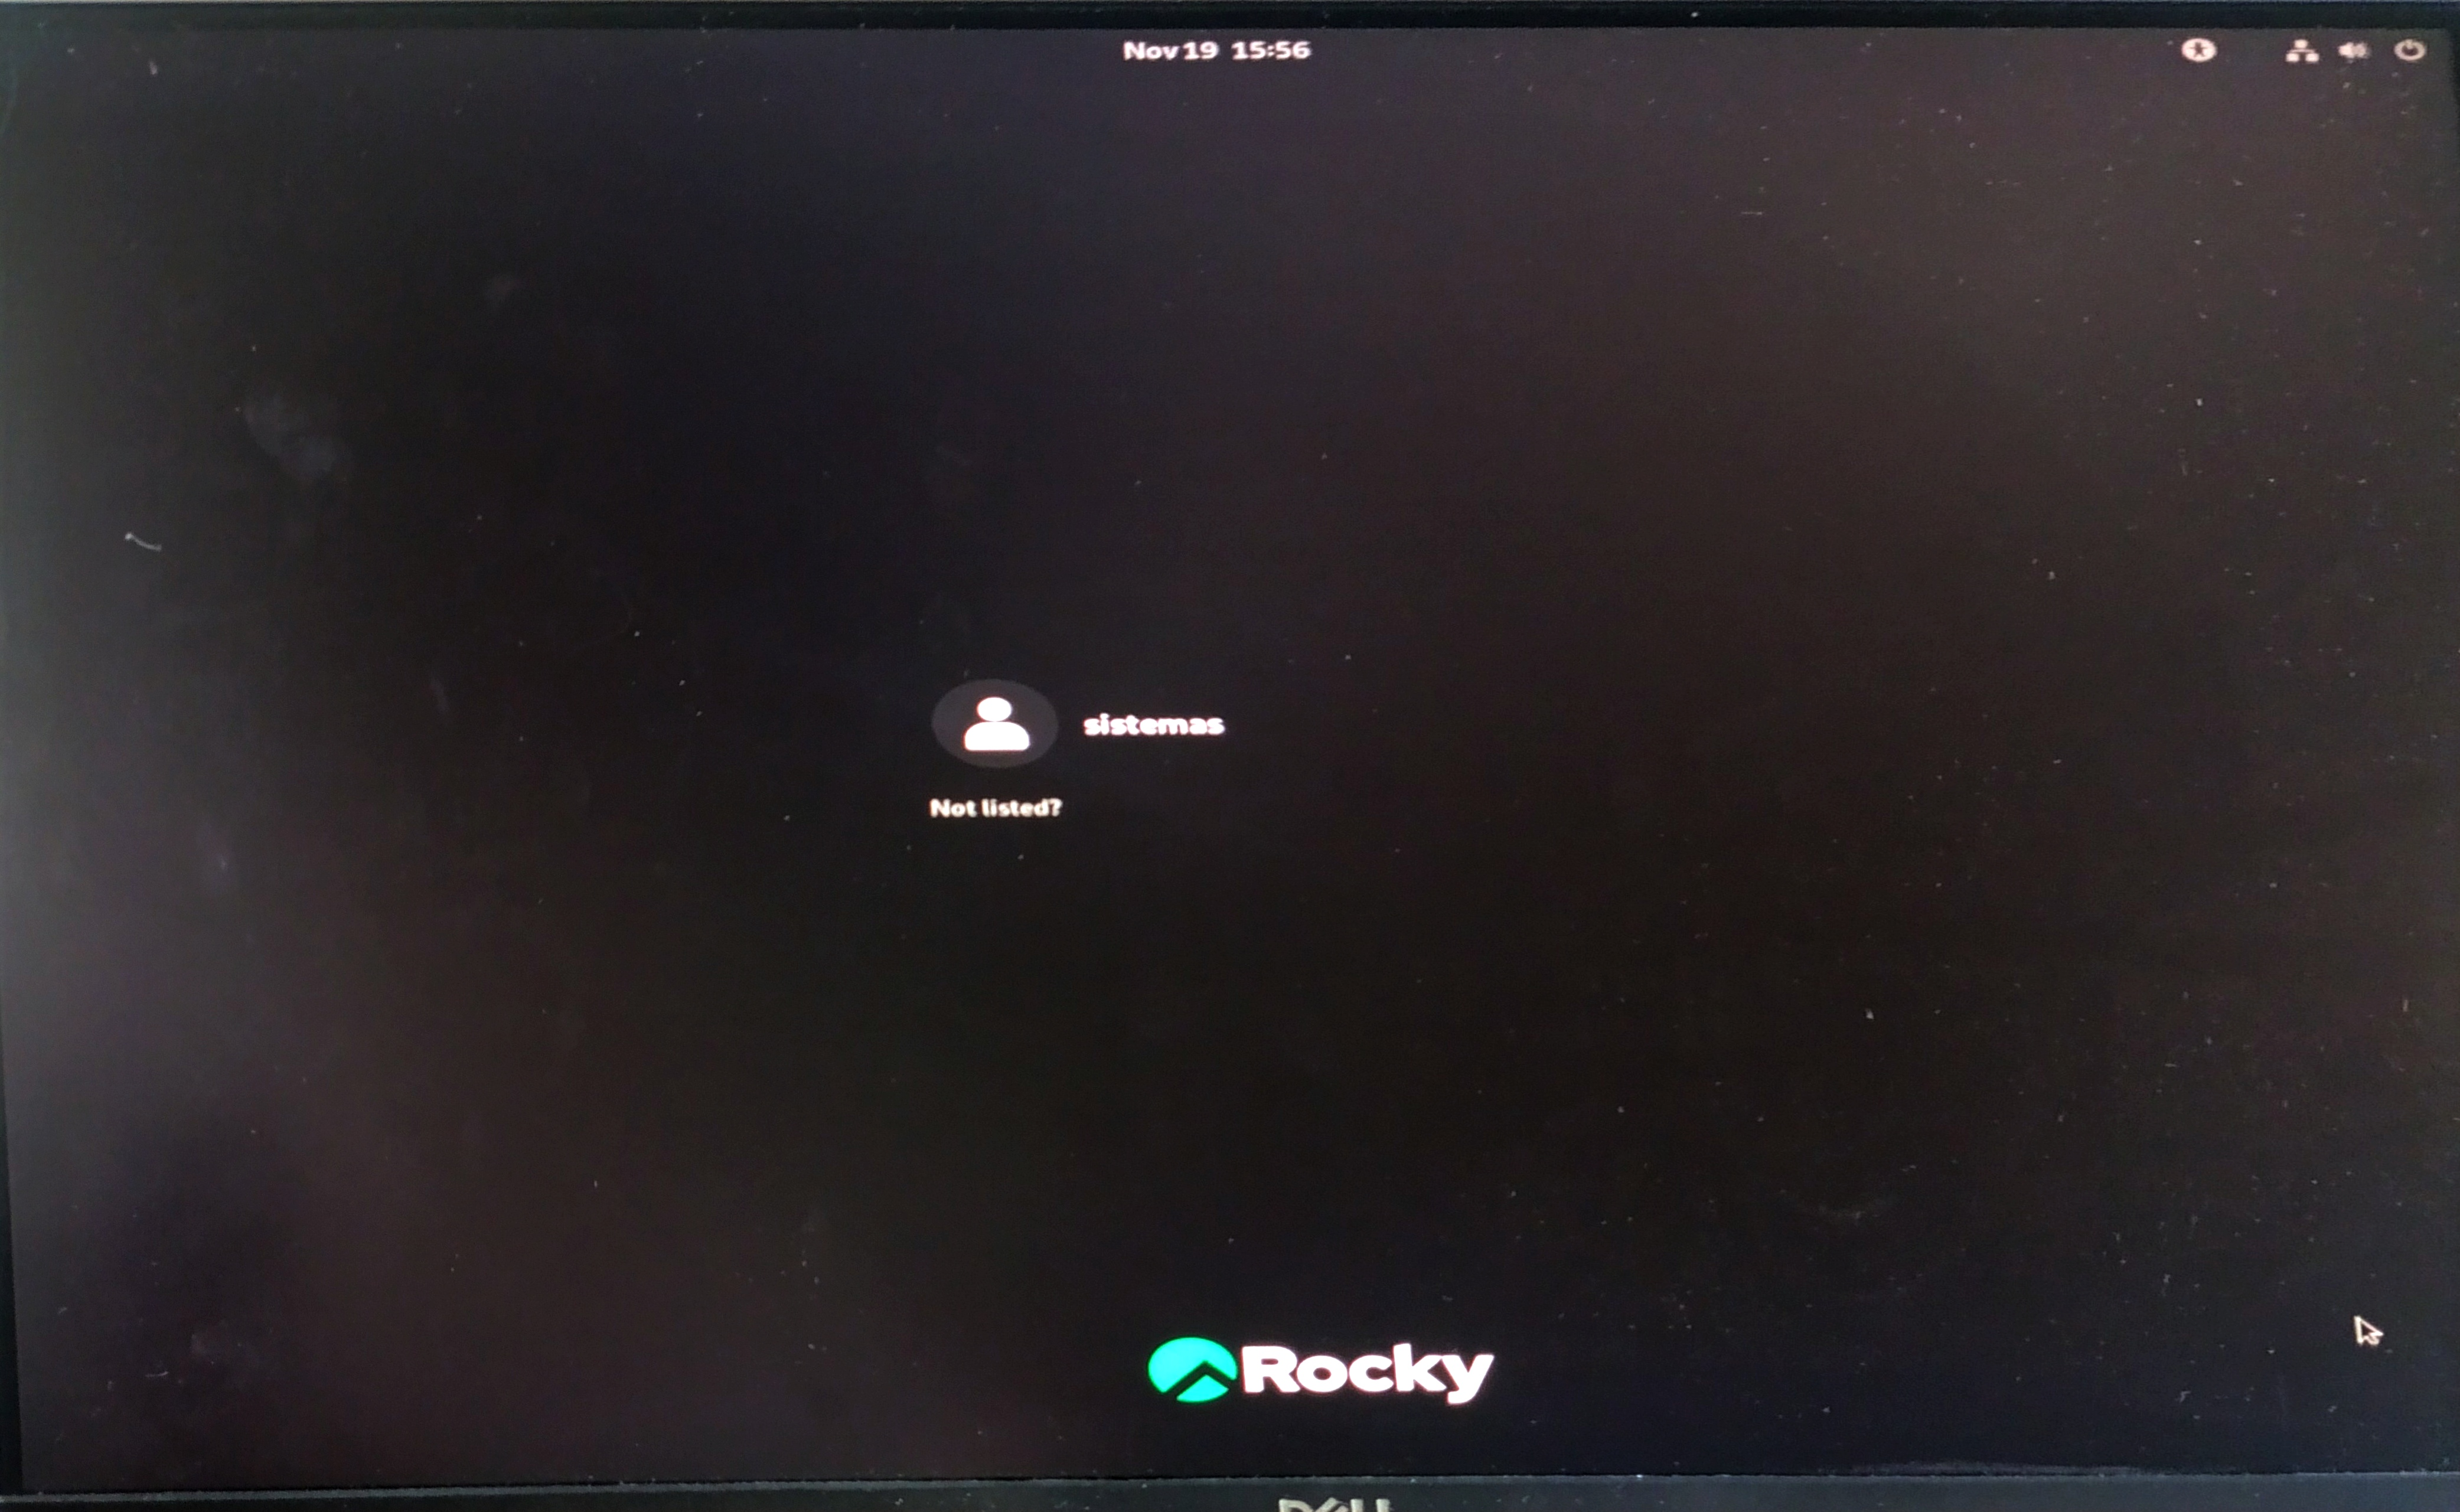
\includegraphics[width=0.75\textwidth] {images/HPC/Rocky/gui_login.jpg}
  \caption{Pantalla de inicio de sesión gráfica en el nodo master.}
  \label{fig:gui_login}
\end{figure}

\begin{figure}[H]
  \centering
  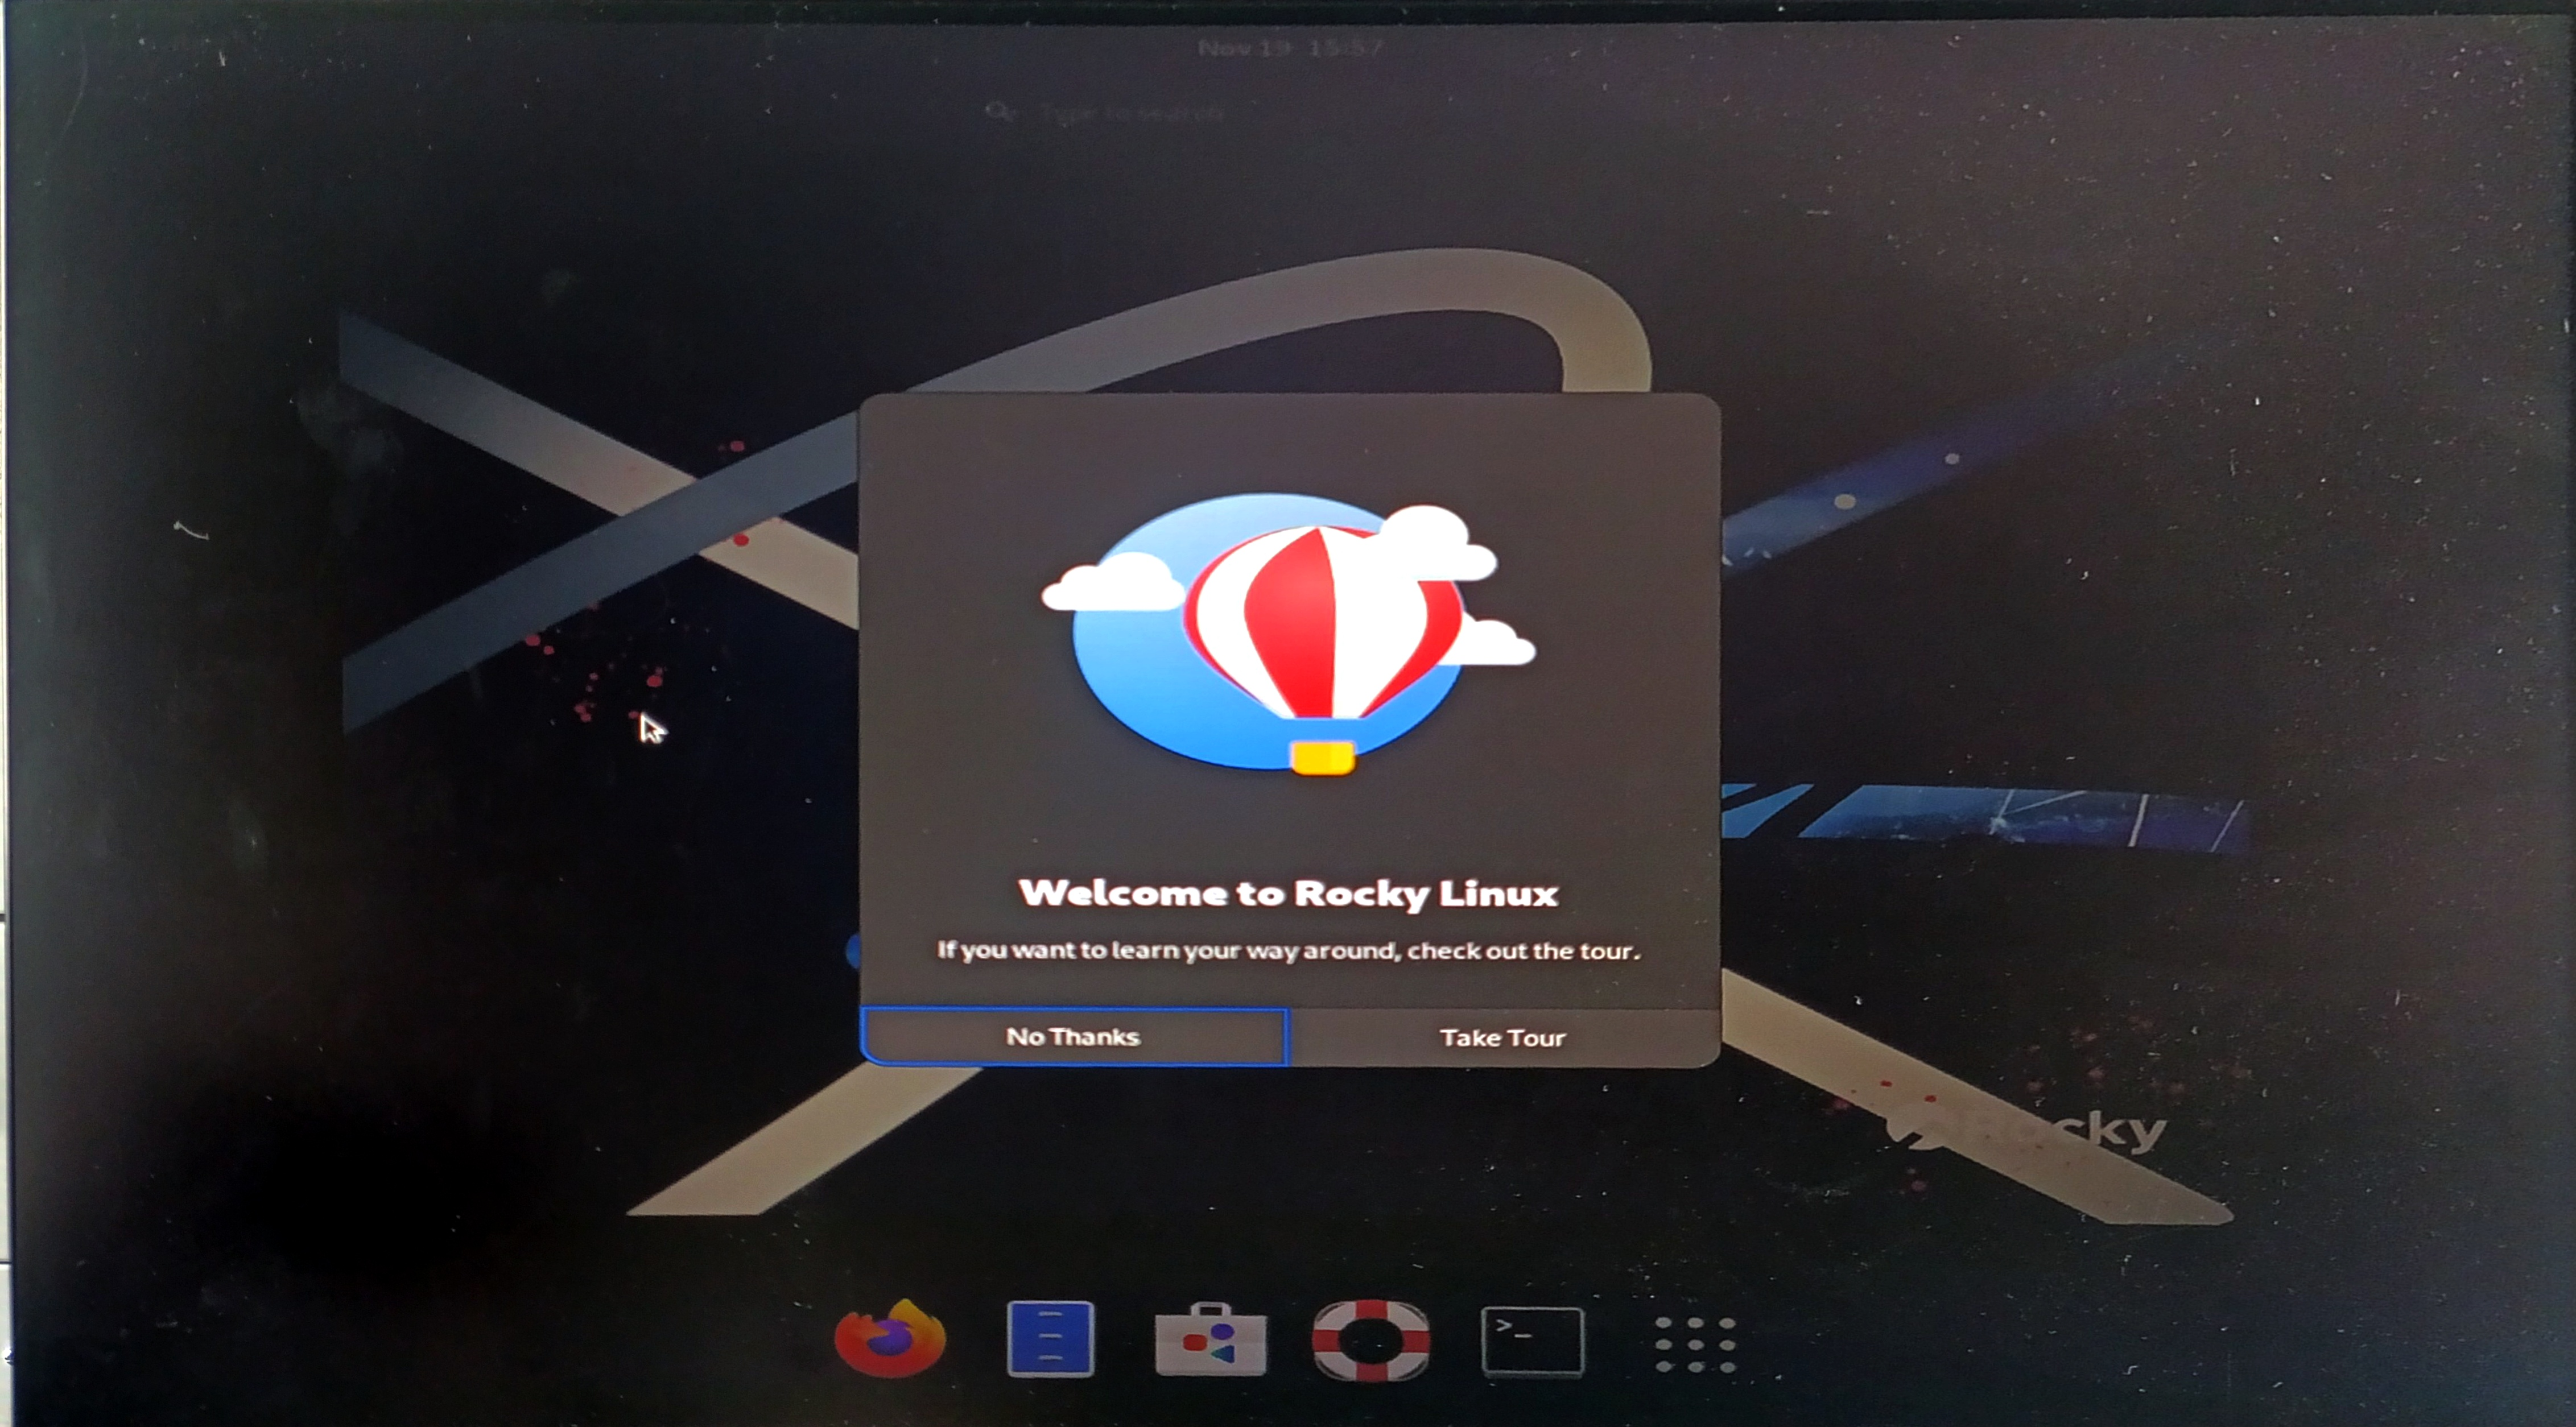
\includegraphics[width=0.75\textwidth] {images/HPC/Rocky/rocky_welcome.jpg}
  \caption{Pantalla de bienvenida del entorno gráfico en Rocky Linux.}
  \label{fig:gui_login}
\end{figure}

Se recomienda seguir el tour si se no se está familiarizado con el entorno GNOME en Linux.

\section{Instalación de Rocky Linux 9.x Minimal en los nodos worker (sin GUI)}
\label{subsec:instalacion_workers}

En los nodos \textit{worker} se repite el mismo procedimiento de instalación descrito para el nodo \textit{master} (Sección~\ref{subsec:instalacion_master}), usando la misma ISO \texttt{Rocky-9-latest-x86\_64-minimal.iso} y el mismo instalador (Anaconda). La intención es mantener consistencia en el sistema base del clúster para simplificar soporte y administración. \cite{rocky_install_9_6}

La diferencia principal es que en los \textit{workers} no se instala interfaz gráfica. Los \textit{workers} se administran remotamente desde el \textit{master}, por lo que una instalación mínima reduce paquetes innecesarios, facilita mantenimiento y disminuye la superficie de ataque del sistema al evitar componentes adicionales. \cite{redhat_linux_security_tips,redhat_reduce_attack_surface}

\subsubsection*{Diferencias aplicadas respecto a la instalación del master}
Durante la instalación de cada \textit{worker} se mantuvieron las mismas decisiones base (idioma, teclado, zona horaria y usuario administrativo), y se aplicaron estas diferencias:

\begin{enumerate}
  \item En \textbf{Software Selection}, se mantuvo \textbf{Minimal Install} y no se instaló GUI en los \textit{workers}.
  % \begin{figure}[H]
  %   \centering
  %   \includegraphics[width=0.92\textwidth]{images/configuración_del_entorno/w01_software_minimal.png}
  %   \caption{Selección de software base: Minimal Install en un nodo worker.}
  %   \label{fig:w01_software_minimal}
  % \end{figure}

  \item En \textbf{Network \& Hostname}, se definió un nombre de host único por nodo:
  \begin{itemize}
    \item \texttt{worker1} para el primer \textit{worker}.
    \item \texttt{worker2} para el segundo \textit{worker}.
  \end{itemize}
  % \begin{figure}[H]
  %   \centering
  %   \includegraphics[width=0.92\textwidth]{images/configuración_del_entorno/w01_network_hostname_worker1.png}
  %   \caption{Hostname configurado como \texttt{worker1} durante la instalación.}
  %   \label{fig:w01_network_hostname_worker1}
  % \end{figure}
  %
  % \begin{figure}[H]
  %   \centering
  %   \includegraphics[width=0.92\textwidth]{images/configuración_del_entorno/w02_network_hostname_worker2.png}
  %   \caption{Hostname configurado como \texttt{worker2} durante la instalación.}
  %   \label{fig:w02_network_hostname_worker2}
  % \end{figure}
\end{enumerate}

Al finalizar la instalación, los \textit{workers} iniciaron en modo consola (sin entorno gráfico), lo cual evidenció que la instalación correspondía a \textit{Minimal Install}.

% \begin{figure}[H]
%   \centering
%   \includegraphics[width=0.92\textwidth]{images/configuración_del_entorno/w01_first_boot_console.png}
%   \caption{Primer arranque de un nodo worker en modo consola (sin GUI).}
%   \label{fig:w01_first_boot_console}
% \end{figure}

\subsubsection*{Verificaciones post-instalación realizadas en cada worker}
Después del primer inicio de sesión en cada \textit{worker}, se realizaron verificaciones rápidas para confirmar que la instalación quedó operativa y consistente con el clúster.

\begin{enumerate}
  \item Se confirmó el nombre del host configurado:
\begin{verbatim}
hostnamectl
\end{verbatim}
La salida mostró el hostname esperado (por ejemplo, \texttt{worker1} o \texttt{worker2}), lo cual confirmó que el identificador del nodo quedó aplicado correctamente.

\begin{figure}[H]
  \centering
  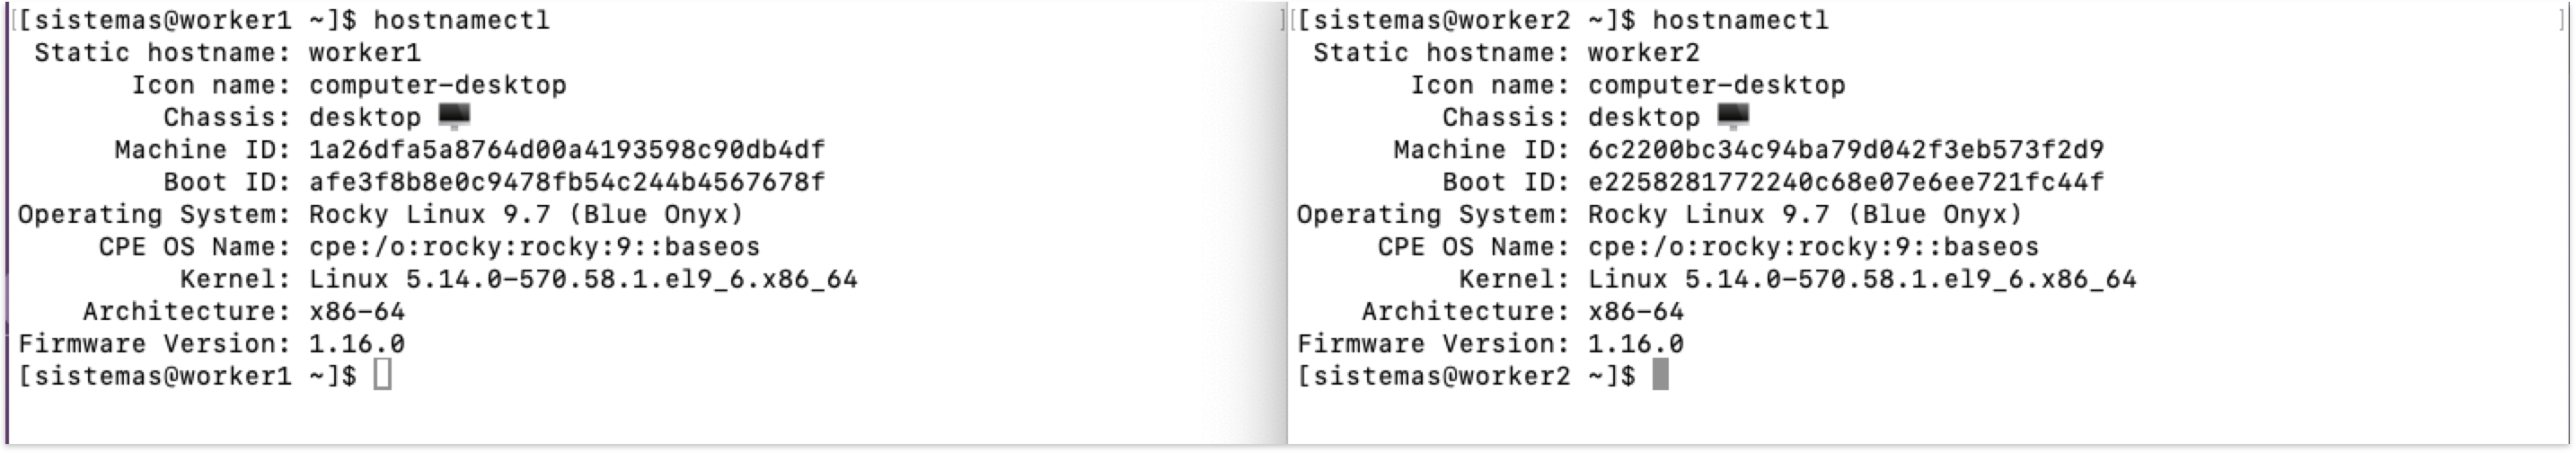
\includegraphics[width=0.92\textwidth]{images/HPC/Rocky/hostnamectl w1 y w2.png}
  \caption{Verificación del hostname con hostnamectl en \texttt{worker1 y worker2}.}
  \label{fig:hostnamectl_worker1_worker2}
\end{figure}


  \item Se confirmó la versión del sistema operativo instalada:
\begin{verbatim}
cat /etc/os-release
\end{verbatim}
La salida mostró Rocky Linux 9.x, consistente con la versión usada en el \textit{master}.

\begin{figure}[H]
  \centering
  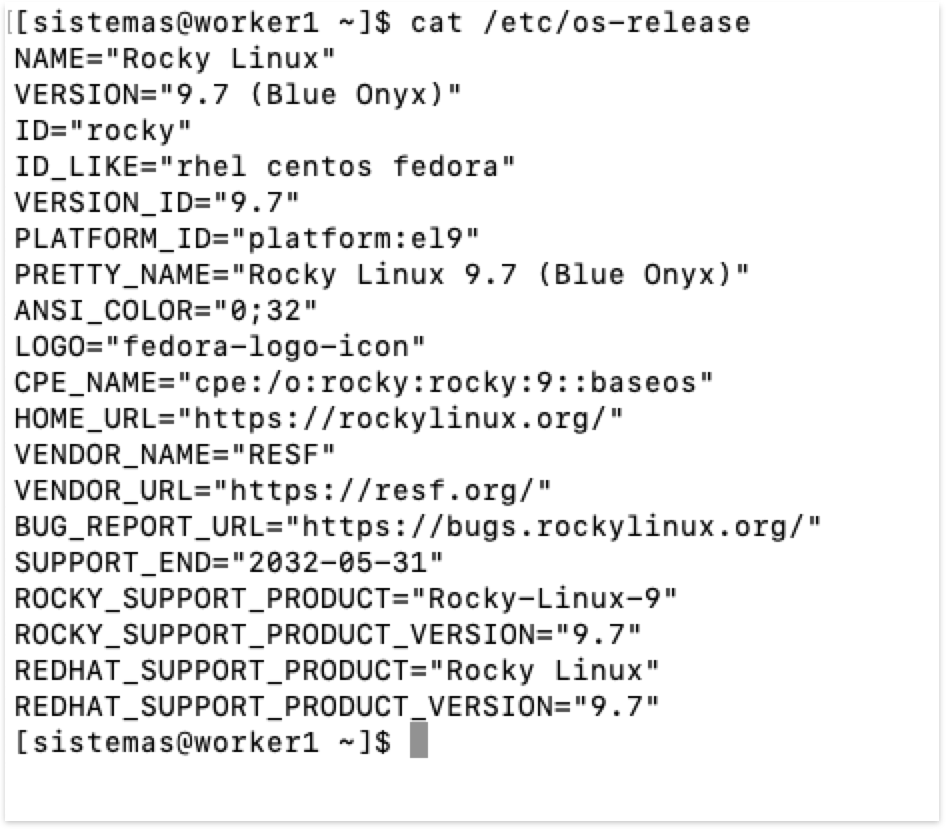
\includegraphics[width=0.5\textwidth]{images/HPC/Rocky/os-release.png}
  \caption{Verificación de versión del sistema (\texttt{/etc/os-release}) en un nodo worker.}
  \label{fig:w01_os_release}
\end{figure}

  \item Se verificaron discos, particiones y montajes:
\begin{verbatim}
lsblk
df -h
\end{verbatim}
Estas salidas permitieron confirmar que el disco del sistema tenía particiones montadas correctamente y que el nodo contaba con espacio disponible para operación. En caso de haberse definido puntos de montaje adicionales en el \textit{worker}, estos también se observaron reflejados en \texttt{df -h}.

\begin{figure}[H]
  \centering
  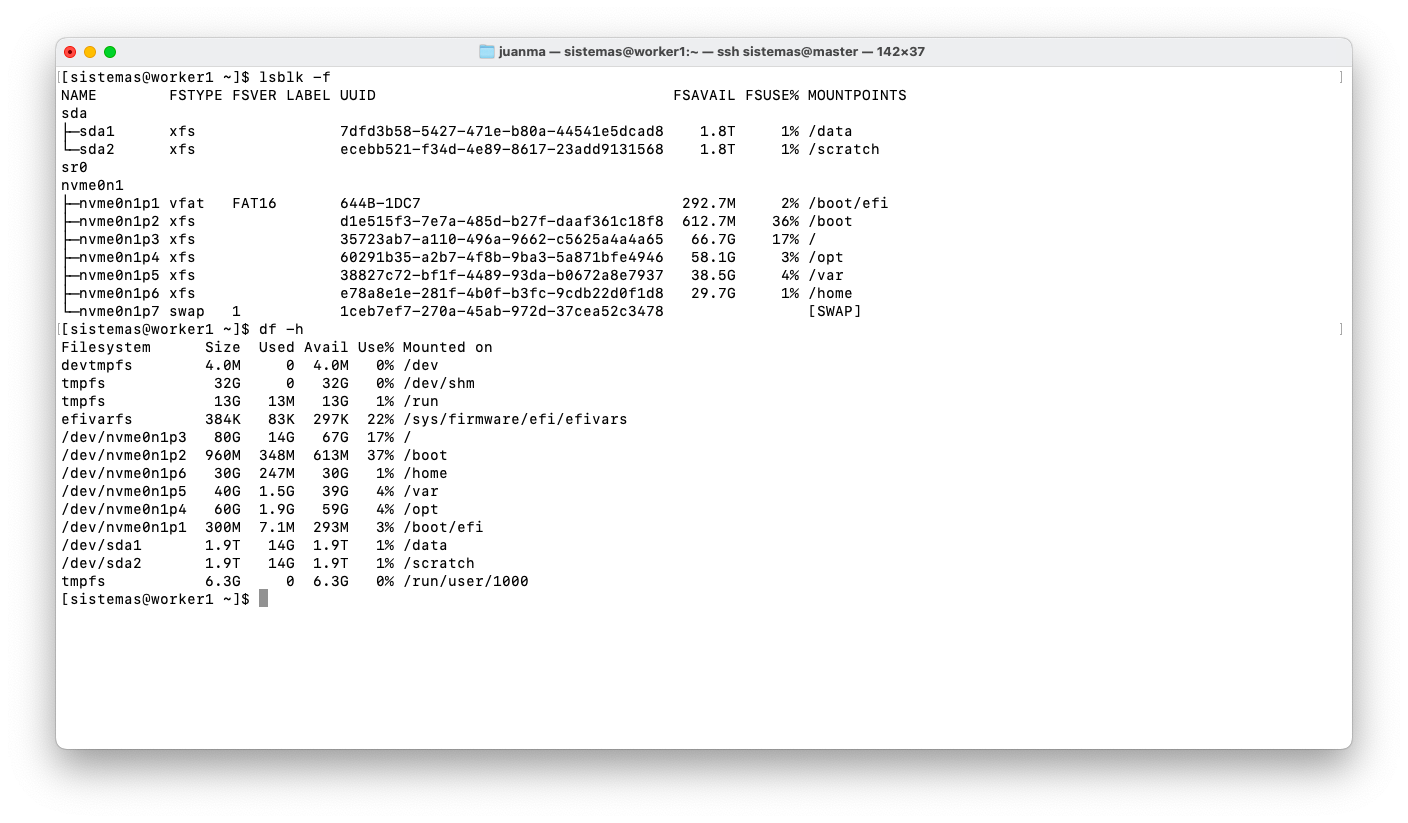
\includegraphics[width=0.92\textwidth]{images/HPC/Rocky/particiones lsblk df.png}
  \caption{Verificación de discos, espacio y puntos de montaje en un nodo worker.}
  \label{fig:w01_storage_check}
\end{figure}
\end{enumerate}

\section{Red de administración del clúster (red ``global'')}
\label{sec:red_global}

Esta sección describe cómo se verificó la conectividad de administración del clúster. En este proyecto se denomina \textit{red global} a la red institucional existente que permite acceder por SSH a cada nodo (por ejemplo, para administración inicial). Esta red es distinta de la red interna del clúster (que se configura más adelante para aislar los \textit{workers}).

\subsection{Verificación de interfaz y ruta por defecto en el nodo master}
\label{subsec:verificacion_red_master}

Los nodos del clúster tienen varias interfaces de red (varios puertos físicos). En un entorno con múltiples interfaces, identificar la interfaz correcta es importante porque una configuración aplicada en la interfaz equivocada puede dejar el equipo sin acceso remoto. Por ello, antes de configurar cualquier automatización o servicios, se verifica qué interfaz está conectada a la red de administración y cuál es la ruta por defecto (el camino que usa el equipo para salir a otras redes). \cite{iproute2_ip,iproute2_ip_route}

\subsubsection*{Identificación de la interfaz activa (caso real: \texttt{eno1})}
\begin{enumerate}
  \item Se abrió una terminal en el nodo \textit{master}.
  \item Se listaron las interfaces y direcciones IP:
\end{enumerate}

\begin{verbatim}
ip a
\end{verbatim}

\begin{figure}[H]
  \centering
  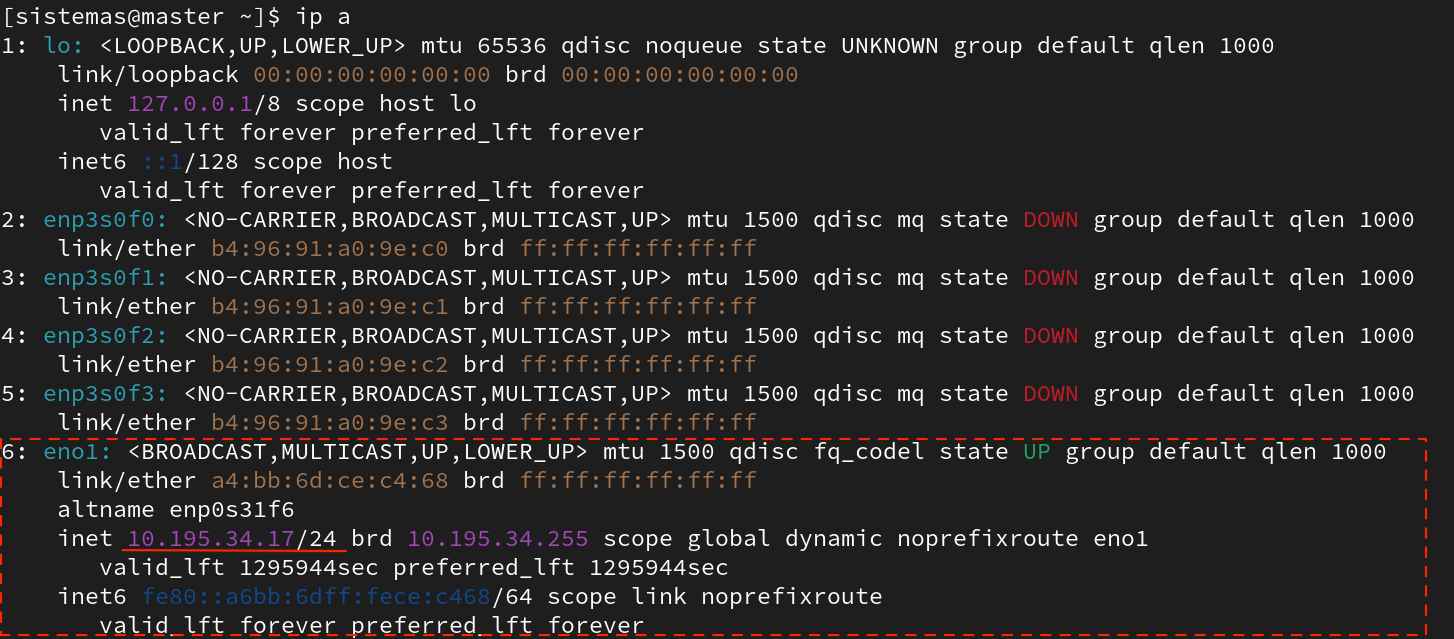
\includegraphics[width=0.92\textwidth]{images/HPC/Rocky/ip_a_master_base.png}
  \caption{Salida de \texttt{ip a} en el master, destacando la interfaz \texttt{eno1} y la IP de administración.}
  \label{fig:b01_ip_a_master}
\end{figure}

En la salida se observó que la interfaz conectada a la red de administración era \texttt{eno1}. En esa misma interfaz se evidenció una dirección IPv4 dentro del segmento \texttt{10.195.34.0/24}. El instalador y el sistema mostraron que la IP usada para el \textit{master} fue \texttt{10.195.34.17/24} en \texttt{eno1}.


\subsubsection*{Verificación de la ruta por defecto (gateway)}
Una \textit{ruta por defecto} indica a qué puerta de enlace (\textit{gateway}) debe enviarse el tráfico destinado a redes que no son locales. En términos prácticos, si existe una ruta por defecto válida, el nodo normalmente puede comunicarse con otros segmentos de red y servicios externos (según las políticas de la red).

\begin{enumerate}
  \item Se consultó la tabla de rutas:
\end{enumerate}

\begin{verbatim}
ip route
\end{verbatim}

\begin{figure}
  \centering
  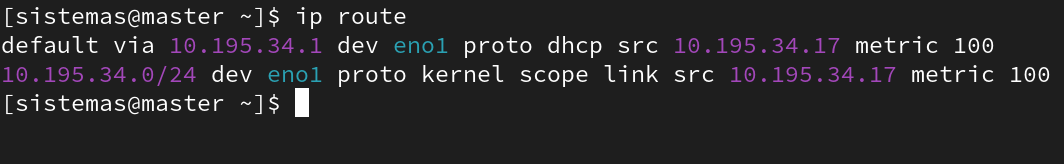
\includegraphics[width=0.9\textwidth] {images/HPC/Rocky/ip_route_master.png}
  \caption{Salida de \texttt{ip route} en el master mostrando gateway y red local.}
  \label{fig:b02_ip_route_master}
\end{figure}

En la salida se observó la ruta por defecto y el segmento local configurado en la interfaz \texttt{eno1}:

% \begin{verbatim}
% default via 10.195.34.1 dev eno1 proto dhcp src 10.195.34.17 metric 100
% 10.195.34.0/24 dev eno1 proto kernel scope link src 10.195.34.17 metric 100
% \end{verbatim}

Esto confirmó dos aspectos operativos: (1) el gateway fue \texttt{10.195.34.1} y (2) la IP del \textit{master} en la red global fue \texttt{10.195.34.17}. Además, el texto \texttt{proto dhcp} evidenció que la configuración fue obtenida mediante DHCP (asignación automática de red). \cite{iproute2_ip_route}

En redes institucionales es común que una IP obtenida por DHCP se mantenga igual tras reinicios, ya sea porque existe una reserva para el equipo o porque el servidor DHCP renueva la concesión (\textit{lease}) con la misma dirección. Por esa razón, aunque la IP no cambió después de reiniciar, el indicador \texttt{proto dhcp} mostró que el método de asignación es DHCP.

\subsection{Estrategia de direccionamiento en la red de administración (DHCP durante la fase inicial)}
\label{subsec:dhcp_red_global}

En la red de administración del clúster, el direccionamiento puede ser automático (DHCP) o manual (IP estática). En esta fase del proyecto se mantiene DHCP para el nodo \textit{master} mientras se completa la configuración base, porque reduce el riesgo de perder acceso remoto por un error de configuración. En entornos institucionales es común que, aun usando DHCP, una dirección IP se conserve por periodos largos debido a renovaciones de concesión (\textit{lease}) o reservas en el servidor DHCP.

A partir de la tabla de rutas se confirmó que el método activo era DHCP (indicador \texttt{proto dhcp}) y que el tráfico salía por la interfaz correcta (\texttt{eno1}). Con esa evidencia, se decidió no forzar una IP estática en este punto y continuar con la instalación y configuración del clúster sobre la conectividad ya funcional.

% \begin{figure}[h]
%   \centering
%   \includegraphics[width=0.92\textwidth]{images/cap_config_entorno/b03_decision_dhcp.png}
%   \caption{Evidencia de direccionamiento por DHCP en la red global (fragmento de \texttt{ip route} con \texttt{proto dhcp}).}
%   \label{fig:b03_decision_dhcp}
% \end{figure}

Si se requiere documentar el método de configuración desde el gestor de red (NetworkManager), se puede consultar el perfil activo y el parámetro \texttt{ipv4.method}. En NetworkManager, \texttt{ipv4.method=auto} corresponde a asignación automática (por ejemplo, DHCP) y \texttt{ipv4.method=manual} corresponde a configuración estática. \cite{nm_settings_nmcli,rhel9_networking}

\subsubsection*{Consulta opcional del método IPv4 con \texttt{nmcli}}
\begin{enumerate}
  \item Se listan las conexiones activas y el dispositivo asociado:
\end{enumerate}

\begin{verbatim}
nmcli -t -f NAME,DEVICE,STATE connection show --active
\end{verbatim}

% \begin{figure}[h]
%   \centering
%   \includegraphics[width=0.92\textwidth]{images/cap_config_entorno/b04_nmcli_active_connections.png}
%   \caption{Consulta de conexiones activas con \texttt{nmcli connection show --active}.}
%   \label{fig:b04_nmcli_active_connections}
% \end{figure}

\begin{enumerate}
  \setcounter{enumi}{1}
  \item Se consulta el método IPv4 del perfil activo (reemplazando \texttt{<CONEXION>} por el nombre real mostrado en el paso anterior):
\end{enumerate}

\begin{verbatim}
nmcli -f ipv4.method,ipv4.addresses,ipv4.gateway connection show "<CONEXION>"
\end{verbatim}

En la salida se espera observar \texttt{ipv4.method: auto} cuando el nodo está configurado por DHCP, además de la dirección asignada y el gateway del perfil. Esto permite respaldar documentalmente el método de direccionamiento sin depender solo de la tabla de rutas. \cite{nm_settings_nmcli}

\section{Acceso remoto al nodo master (SSH sobre la red de administración)}
\label{sec:ssh_master}

Esta sección describe cómo se habilita y verifica el acceso remoto al nodo \textit{master} mediante SSH (\textit{Secure Shell}). SSH permite administrar el clúster desde otro computador sin necesidad de estar físicamente frente al equipo, y es un requisito para automatización posterior.

\subsection{Habilitación del servicio SSH en el master}
En Rocky Linux el servicio que acepta conexiones SSH es \texttt{sshd}. Para que el nodo \textit{master} sea administrable remotamente, el servicio debe estar instalado, en ejecución y permitido a través del firewall. \cite{openssh_sshd_config_man,rhel_openssh_secure}

\begin{enumerate}
  \item Se verificó si el servidor OpenSSH estaba instalado y, si era necesario, se instaló:
\end{enumerate}

\begin{verbatim}
sudo dnf -y install openssh-server
\end{verbatim}

% \begin{figure}[h]
%   \centering
%   \includegraphics[width=0.92\textwidth]{images/cap_config_entorno/c01_dnf_install_openssh_server.png}
%   \caption{Instalación del paquete \texttt{openssh-server} en el master.}
%   \label{fig:c01_dnf_install_openssh_server}
% \end{figure}

Después de la instalación, se dejó el servicio habilitado para iniciar automáticamente y se inició de inmediato. La salida de \texttt{systemctl status} mostró el servicio en estado \texttt{active (running)}, lo cual evidenció que el master estaba listo para aceptar conexiones. \cite{rhel_openssh_secure}

\begin{verbatim}
sudo systemctl enable --now sshd
sudo systemctl status sshd --no-pager
\end{verbatim}

% \begin{figure}[h]
%   \centering
%   \includegraphics[width=0.92\textwidth]{images/cap_config_entorno/c02_systemctl_status_sshd.png}
%   \caption{Estado del servicio \texttt{sshd} en ejecución.}
%   \label{fig:c02_systemctl_status_sshd}
% \end{figure}

\begin{enumerate}
  \setcounter{enumi}{1}
  \item Se habilitó el servicio SSH en el firewall del sistema y se recargó la configuración:
\end{enumerate}

\begin{verbatim}
sudo firewall-cmd --permanent --add-service=ssh
sudo firewall-cmd --reload
sudo firewall-cmd --list-services
\end{verbatim}

% \begin{figure}[h]
%   \centering
%   \includegraphics[width=0.92\textwidth]{images/cap_config_entorno/c03_firewalld_add_ssh.png}
%   \caption{Habilitación de SSH en el firewall (\texttt{firewalld}) y verificación de servicios permitidos.}
%   \label{fig:c03_firewalld_add_ssh}
% \end{figure}

En la lista de servicios permitidos se observó \texttt{ssh}, lo cual confirmó que el firewall no bloquearía conexiones entrantes al puerto 22.

\subsection{Conexión desde el computador del usuario hacia el master}
Para conectarse al master se requiere conocer (1) la IP del master en la red de administración y (2) un usuario válido. En este proyecto, el usuario de administración creado fue \texttt{sistemas} y el master usó la IP \texttt{10.195.34.17} sobre la interfaz \texttt{eno1} (Sección~\ref{subsec:verificacion_red_master}). 

\begin{enumerate}
  \item Desde el computador del usuario, se realizó la conexión SSH hacia el master:
\end{enumerate}

\begin{verbatim}
ssh sistemas@10.195.34.17
\end{verbatim}

% \begin{figure}[h]
%   \centering
%   \includegraphics[width=0.92\textwidth]{images/cap_config_entorno/c04_ssh_first_connection.png}
%   \caption{Primera conexión SSH desde el computador del usuario hacia el master.}
%   \label{fig:c04_ssh_first_connection}
% \end{figure}

En la primera conexión es normal que el cliente SSH solicite confirmar la identidad del servidor (huella digital de la llave del host). Al aceptar, el cliente guarda esa huella para detectar cambios futuros. Este comportamiento hace parte del diseño de seguridad de OpenSSH. \cite{openssh_manual}

Al ingresar la contraseña del usuario \texttt{sistemas} (que en este caso también es \texttt{sistemas}), se obtuvo acceso a una sesión remota. Como verificación simple, se ejecutó \texttt{hostname} y se observó \texttt{master}, lo cual confirmó que la sesión correspondía al nodo correcto.

\begin{verbatim}
hostname
\end{verbatim}

% \begin{figure}[h]
%   \centering
%   \includegraphics[width=0.92\textwidth]{images/cap_config_entorno/c05_hostname_master_remote.png}
%   \caption{Verificación rápida del nodo remoto con \texttt{hostname}.}
%   \label{fig:c05_hostname_master_remote}
% \end{figure}

\subsection{Autenticación por llaves SSH (usuario $\rightarrow$ master y master $\rightarrow$ workers)}
\label{subsec:ssh_keys}

En esta etapa se configura autenticación por llaves SSH para reducir dependencia de contraseñas y habilitar administración automatizada. En SSH, la autenticación por llaves funciona con un par criptográfico: una llave privada que permanece protegida en el equipo que inicia la conexión y una llave pública que se instala en el servidor dentro de \texttt{\textasciitilde/.ssh/authorized\_keys}. \cite{man_ssh_keygen,redhat_key_based_auth_blog,rhel_key_pairs_ssh}

\subsubsection*{Generación de la llave en el computador del usuario (para acceder al master)}
\begin{enumerate}
  \item En el computador del usuario se generó un par de llaves Ed25519 para el acceso al \textit{master}:
\end{enumerate}

\begin{verbatim}
ssh-keygen -t ed25519
\end{verbatim}

Este comando creó (por defecto) dos archivos en \texttt{\textasciitilde/.ssh/}: la llave privada \texttt{id\_ed25519} y la llave pública \texttt{id\_ed25519.pub}. \cite{man_ssh_keygen}

% \begin{figure}[h]
%   \centering
%   \includegraphics[width=0.92\textwidth]{images/cap_config_entorno/d01_ssh_keygen_local.png}
%   \caption{Generación de la llave SSH en el computador del usuario (ssh-keygen).}
%   \label{fig:d01_ssh_keygen_local}
% \end{figure}

\begin{enumerate}
  \setcounter{enumi}{1}
  \item Se verificó que los archivos quedaron creados y con permisos restrictivos (la llave privada no debe ser legible por otros usuarios):
\end{enumerate}

\begin{verbatim}
ls -l ~/.ssh/id_ed25519 ~/.ssh/id_ed25519.pub
\end{verbatim}

En la salida se observó que la llave privada tenía permisos restrictivos (típicamente \texttt{-rw-------}). Esto es importante porque OpenSSH puede rechazar llaves privadas con permisos inseguros. \cite{redhat_key_based_auth_blog}

% \begin{figure}[h]
%   \centering
%   \includegraphics[width=0.92\textwidth]{images/cap_config_entorno/d02_ls_l_ssh_keys_local.png}
%   \caption{Verificación de existencia y permisos de llaves en \texttt{\textasciitilde/.ssh/}.}
%   \label{fig:d02_ls_l_ssh_keys_local}
% \end{figure}

\subsubsection*{Instalación de la llave pública en el master}
Para instalar la llave pública de forma segura y controlada se utilizó \texttt{ssh-copy-id}, herramienta incluida con OpenSSH que agrega la llave pública al archivo \texttt{authorized\_keys} del usuario remoto. \cite{man_ssh_copy_id}

\begin{enumerate}
  \item Desde el computador del usuario se copió la llave pública al usuario \texttt{sistemas} del master:
\end{enumerate}

\begin{verbatim}
ssh-copy-id -i ~/.ssh/id_ed25519.pub sistemas@10.195.34.17
\end{verbatim}

Durante este paso, el sistema solicitó la contraseña del usuario remoto para permitir la instalación inicial de la llave (esto es esperado con \texttt{ssh-copy-id}). \cite{man_ssh_copy_id}

% \begin{figure}[h]
%   \centering
%   \includegraphics[width=0.92\textwidth]{images/cap_config_entorno/d03_ssh_copy_id_to_master.png}
%   \caption{Instalación de la llave pública en el master con \texttt{ssh-copy-id}.}
%   \label{fig:d03_ssh_copy_id_to_master}
% \end{figure}

\begin{enumerate}
  \setcounter{enumi}{1}
  \item Se probó el acceso por llave (sin contraseña) ejecutando un comando remoto:
\end{enumerate}

\begin{verbatim}
ssh sistemas@10.195.34.17 "hostname"
\end{verbatim}

En la salida se observó \texttt{master}. La ausencia de solicitud de contraseña evidenció que la autenticación por llave quedó funcionando.

% \begin{figure}[h]
%   \centering
%   \includegraphics[width=0.92\textwidth]{images/cap_config_entorno/d04_ssh_master_hostname_no_password.png}
%   \caption{Prueba de acceso por llave al master (sin contraseña) ejecutando \texttt{hostname}.}
%   \label{fig:d04_ssh_master_hostname_no_password}
% \end{figure}

\subsubsection*{Llave desde el master hacia los workers (para administración del clúster)}
En el clúster, el nodo \textit{master} se usa como punto central de administración. Por ello, se configuró también autenticación por llaves desde el \textit{master} hacia cada \textit{worker}, de modo que el \textit{master} pueda conectarse y ejecutar comandos remotos de forma no interactiva (requisito práctico para Ansible). \cite{rhel_key_pairs_ssh}

\begin{enumerate}
  \item En el \textit{master}, iniciando sesión como \texttt{sistemas}, se generó una llave Ed25519 destinada a conexiones hacia los \textit{workers}:
\end{enumerate}

\begin{verbatim}
ssh-keygen -t ed25519
\end{verbatim}

% \begin{figure}[h]
%   \centering
%   \includegraphics[width=0.92\textwidth]{images/cap_config_entorno/d05_ssh_keygen_on_master.png}
%   \caption{Generación de llave SSH en el master para conexión a workers.}
%   \label{fig:d05_ssh_keygen_on_master}
% \end{figure}

\begin{enumerate}
  \setcounter{enumi}{1}
  \item Se instaló la llave pública del master en cada \textit{worker}. Se usó la dirección alcanzable de cada worker en la red de administración (por DHCP) o su hostname si ya resolvía:
\end{enumerate}

\begin{verbatim}
ssh-copy-id -i ~/.ssh/id_ed25519.pub sistemas@worker1
ssh-copy-id -i ~/.ssh/id_ed25519.pub sistemas@worker2
\end{verbatim}

% \begin{figure}[h]
%   \centering
%   \includegraphics[width=0.92\textwidth]{images/cap_config_entorno/d06_ssh_copy_id_to_workers.png}
%   \caption{Instalación de la llave pública del master en workers con \texttt{ssh-copy-id}.}
%   \label{fig:d06_ssh_copy_id_to_workers}
% \end{figure}

\begin{enumerate}
  \setcounter{enumi}{2}
  \item Se verificó la conexión por llave desde el master hacia cada worker ejecutando un comando remoto:
\end{enumerate}

\begin{verbatim}
ssh sistemas@worker1 "hostname"
ssh sistemas@worker2 "hostname"
\end{verbatim}

En la salida se observó el hostname correspondiente (\texttt{worker1} y \texttt{worker2}). Esto evidenció que (1) existía conectividad por SSH y (2) la autenticación por llaves quedó operativa.

% \begin{figure}[h]
%   \centering
%   \includegraphics[width=0.92\textwidth]{images/cap_config_entorno/d07_ssh_workers_hostname_no_password.png}
%   \caption{Prueba de acceso por llave desde el master hacia workers (sin contraseña) ejecutando \texttt{hostname}.}
%   \label{fig:d07_ssh_workers_hostname_no_password}
% \end{figure}


\section{Resumen de la configuración realizada hasta este punto}
\label{sec:resumen_configuracion_hasta_ahora}

El clúster quedó con un sistema base consistente y una vía de administración funcional. Se instaló Rocky Linux 9.x en todos los nodos usando la imagen \textit{Minimal}, con particionado manual para controlar el uso del almacenamiento y asegurar que el sistema operativo y los espacios de trabajo quedaran separados. En el nodo \textit{master} se definió el esquema en \texttt{nvme0n1} para el sistema (\texttt{/}, \texttt{/var}, \texttt{/opt}, \texttt{/home}, \texttt{/boot} y \texttt{/boot/efi}) y se reservaron volúmenes de alta capacidad en \texttt{sda} para \texttt{/data} y \texttt{/scratch}, lo que facilita organizar datos persistentes y archivos temporales de trabajo sin comprometer el sistema.

La conectividad de administración (\textit{red global}) quedó verificada en el \textit{master}, identificando la interfaz utilizada (\texttt{eno1}) y confirmando la salida por una ruta por defecto válida. Se mantuvo el direccionamiento por DHCP durante la fase inicial para disminuir el riesgo de perder acceso remoto, priorizando estabilidad operativa mientras se avanzaba en la configuración del clúster.

En cuanto al acceso remoto, se habilitó el servicio SSH en el \textit{master} y se garantizó que fuera alcanzable a través del firewall. Cuando fue necesario para recuperar y mantener acceso durante la fase inicial, se habilitó autenticación por contraseña en SSH. Posteriormente, se migró la administración a autenticación por llaves SSH, primero desde el computador del usuario hacia el \textit{master}, y luego desde el \textit{master} hacia los \textit{workers}. Esta transición dejó el clúster listo para administración no interactiva desde el nodo \textit{master}, requisito para automatización y orquestación con herramientas como Ansible.

Finalmente, se estandarizó la instalación de los \textit{workers} manteniendo \textit{Minimal Install} y sin interfaz gráfica, ya que estos nodos están diseñados para ser controlados remotamente desde el \textit{master}. Esto reduce componentes innecesarios en los nodos de cómputo y simplifica el mantenimiento del clúster.

A partir de esta base, el siguiente paso es introducir automatización: definir un inventario de hosts, estandarizar variables de conexión, y ejecutar verificaciones remotas de forma repetible (por ejemplo, pruebas de conectividad y recolección de estado) utilizando Ansible.

% ==========================================================
% Archivo: chapters/ansible.tex
% Capítulo: Automatización del clúster con Ansible
% ==========================================================

\chapter{Automatización del clúster con Ansible}
\label{chap:ansible}

Este capítulo presenta Ansible como herramienta de automatización para administración de infraestructura. Primero se explica qué es, cómo funciona y cómo se organiza un proyecto típico. Después se muestran ejemplos independientes (no ligados todavía a la implementación del clúster). En la siguiente sección del capítulo se documenta la implementación realizada en la práctica para este proyecto.

% \begin{figure}[h]
%   \centering
%   \includegraphics[width=0.92\textwidth]{images/cap_ansible/a00_portada_capitulo.png}
%   \caption{Imagen introductoria del capítulo (opcional).}
%   \label{fig:ansible_intro}
% \end{figure}

\section{¿Qué es Ansible y por qué se usa en un clúster?}
\label{sec:ansible_que_es}

Ansible es una herramienta de automatización para administrar múltiples equipos de forma centralizada. En lugar de conectarse manualmente a cada nodo para repetir acciones (instalar paquetes, modificar archivos de configuración, habilitar servicios, montar directorios), Ansible permite describir esas acciones y ejecutarlas de manera consistente sobre un conjunto de equipos.

En un clúster, esta forma de trabajo es especialmente útil porque:
\begin{itemize}
  \item Reduce errores humanos al repetir procedimientos.
  \item Facilita mantener los nodos consistentes entre sí.
  \item Permite re-ejecutar configuraciones cuando un nodo se reinstala o se agrega un nuevo nodo.
\end{itemize}

Ansible es \textit{agentless}: no requiere instalar un ``agente'' permanente en los nodos administrados. En Linux, normalmente se conecta usando SSH desde un nodo de control hacia los nodos gestionados. \cite{rh_how_ansible_works,ansible_installation_guide}

\section{Cómo funciona Ansible}
\label{sec:ansible_como_funciona}

\subsection{Nodos y modelo de ejecución}
\label{subsec:ansible_nodos}

Ansible trabaja con dos roles principales:
\begin{itemize}
  \item \textbf{Nodo de control (control node):} equipo desde el cual se ejecutan los comandos y playbooks de Ansible.
  \item \textbf{Nodos gestionados (managed nodes):} equipos sobre los cuales se aplican las tareas.
\end{itemize}

En este proyecto, típicamente el \textit{master} cumple el rol de nodo de control para administrar los \textit{workers}. La comunicación ocurre por SSH y Ansible ejecuta módulos remotos (generalmente mediante Python en el nodo gestionado). \cite{ansible_installation_guide,rh_how_ansible_works}

\begin{figure}[H]
  \centering
  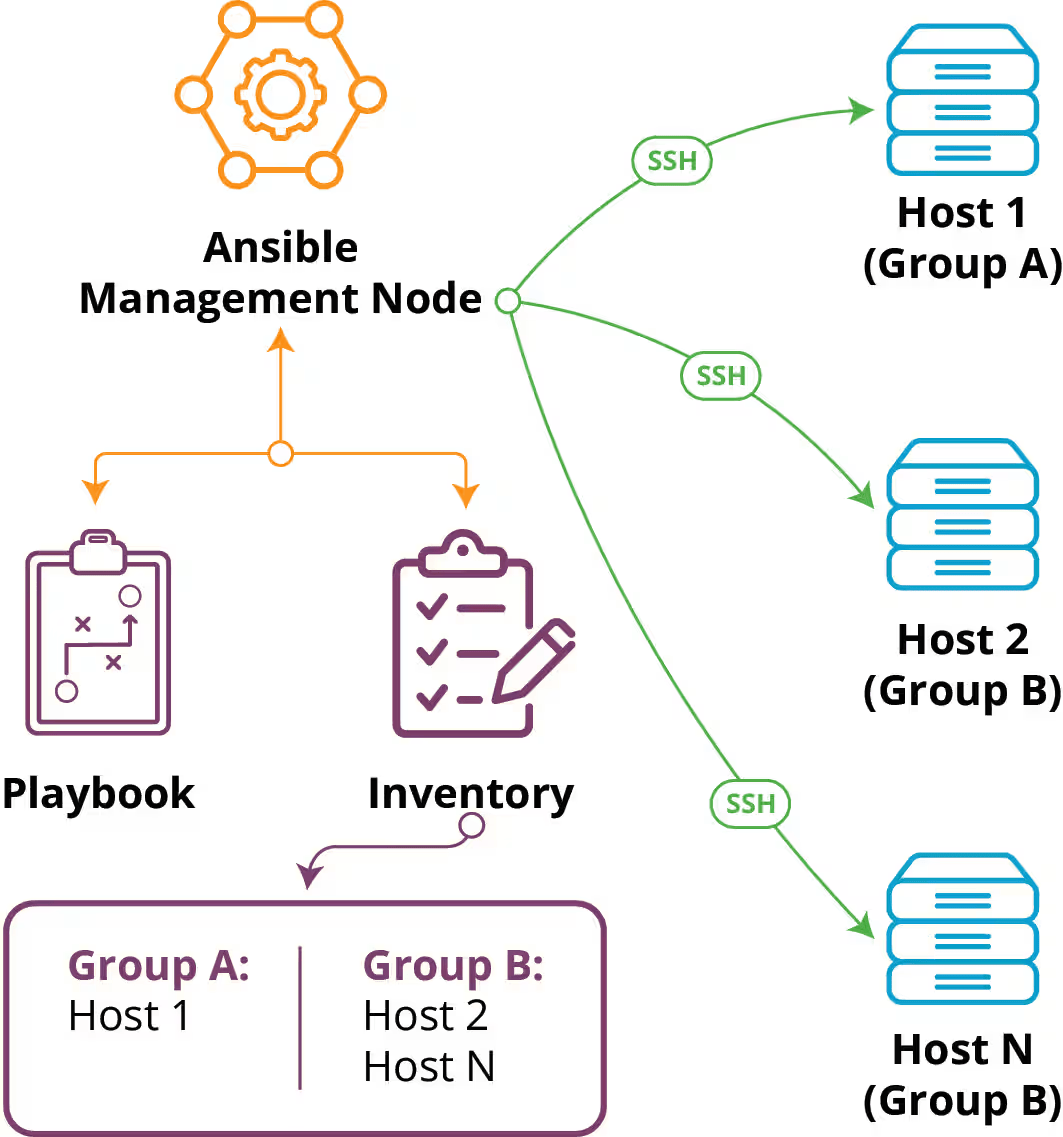
\includegraphics[width=0.5\textwidth]{images/ansible/Ansible diagrama.png}
  \caption{Esquema conceptual: nodo de control ejecutando tareas sobre nodos gestionados por SSH.}
  \label{fig:ansible_control_managed}
\end{figure}

\subsection{Inventario}
\label{subsec:ansible_inventario}

El \textbf{inventario} es la lista de equipos que Ansible administra y cómo se agrupan. Los formatos más comunes son INI y YAML. En el inventario se definen hosts, grupos (por ejemplo, \texttt{workers}) y variables de conexión. \cite{ansible_inventory_intro}

\subsection{Módulos, tareas y estado deseado}
\label{subsec:ansible_modulos}

Ansible ejecuta \textbf{módulos} (pequeñas unidades de trabajo) como ``instalar un paquete'', ``copiar un archivo'' o ``habilitar un servicio''. Muchos módulos están diseñados para ser \textbf{idempotentes}: si el estado deseado ya se cumple, no realizan cambios. Por eso, ejecutar el mismo playbook varias veces tiende a producir el mismo resultado final. \cite{ansible_modules_intro,ansible_playbooks_intro}

\subsection{Playbooks y roles}
\label{subsec:ansible_playbooks_roles}

Un \textbf{playbook} es un archivo YAML que describe qué tareas se ejecutan, sobre qué hosts, y con qué parámetros. Los playbooks se usan cuando la tarea se necesita repetir y versionar. \cite{ansible_playbooks_intro}

Un \textbf{rol (role)} organiza automatizaciones en una estructura reutilizable (tareas, variables, archivos y plantillas). Esto ayuda a mantener el proyecto ordenado cuando la automatización crece.

\section{Conceptos clave}
\label{sec:ansible_conceptos}

\begin{description}
  \item[Host pattern:] selección de objetivos, por ejemplo \texttt{all}, \texttt{master}, \texttt{workers}.
  \item[Variables:] parámetros para hacer playbooks reutilizables (por ejemplo, nombres de paquetes, rutas, puertos). \cite{ansible_variables}
  \item[Handlers:] acciones que se ejecutan solo si hubo un cambio (por ejemplo, reiniciar un servicio tras modificar su configuración). \cite{ansible_modules_intro}
  \item[Privilege escalation (become):] mecanismo para ejecutar tareas con privilegios elevados (similar a \texttt{sudo}). \cite{ansible_become}
\end{description}

\section{Requisitos mínimos para usar Ansible}
\label{sec:ansible_requisitos}

\subsection{En el nodo de control}
El nodo de control requiere Ansible instalado y un entorno Python compatible. \cite{ansible_installation_guide}

\subsection{En los nodos gestionados}
Los nodos gestionados no requieren Ansible instalado, pero normalmente requieren:
\begin{itemize}
  \item Acceso por SSH con una cuenta de usuario válida y un shell POSIX interactivo.
  \item Python para ejecutar el código que Ansible envía temporalmente al nodo (salvo excepciones como algunos módulos de red). \cite{ansible_installation_guide}
\end{itemize}

Por defecto, Ansible asume el uso de llaves SSH (recomendado). Si se usa contraseña, Ansible puede solicitarla con opciones específicas. \cite{ansible_connection_details}

\section{Ejemplos independientes de uso}
\label{sec:ansible_ejemplos}

Los ejemplos de esta sección sirven para entender el uso básico. En la implementación del proyecto se ajustan rutas, nombres de hosts, usuarios y llaves según el clúster.

\subsection{Ejemplo 1: inventario mínimo (INI)}
\label{subsec:ansible_ej1_inventario}

Un inventario INI mínimo define hosts y grupos:

\begin{verbatim}
# inventory.ini (ejemplo)
[master]
master ansible_host=10.195.34.17

[workers]
worker1 ansible_host=10.195.34.21
worker2 ansible_host=10.195.34.22

[all:vars]
ansible_user=sistemas
\end{verbatim}

Este formato permite apuntar a los hosts por nombre (\texttt{worker1}) y conservar la IP como variable (\texttt{ansible\_host}). \cite{ansible_inventory_intro}

% \begin{figure}[h]
%   \centering
%   \includegraphics[width=0.92\textwidth]{images/cap_ansible/a10_inventory_ini.png}
%   \caption{Ejemplo de inventario INI y su ubicación en el proyecto.}
%   \label{fig:ansible_inventory_ini}
% \end{figure}

\subsection{Ejemplo 2: comando ad hoc para probar conectividad (ping)}
\label{subsec:ansible_ej2_ping}

Los \textbf{ad hoc commands} son comandos de una sola tarea que se ejecutan sin escribir playbooks. Son útiles para pruebas rápidas. \cite{ansible_adhoc_intro}

\begin{verbatim}
ansible -i inventory.ini all -m ping
\end{verbatim}

Si la conectividad y credenciales son correctas, cada host responde con \texttt{pong}.

% \begin{figure}[h]
%   \centering
%   \includegraphics[width=0.92\textwidth]{images/cap_ansible/a11_ansible_ping.png}
%   \caption{Ejecución de \texttt{ansible -m ping} y salida esperada.}
%   \label{fig:ansible_ping}
% \end{figure}

\subsection{Ejemplo 3: ejecutar un comando simple en varios hosts}
\label{subsec:ansible_ej3_command}

\begin{verbatim}
ansible -i inventory.ini workers -m command -a "hostname"
\end{verbatim}

Este ejemplo consulta el hostname en todos los \textit{workers}. Para comandos que requieren shell (pipes, redirecciones), se usa el módulo \texttt{shell} con cuidado.

\subsection{Ejemplo 4: playbook mínimo (instalar un paquete)}
\label{subsec:ansible_ej4_playbook}

Un playbook describe tareas repetibles. Este ejemplo asegura que un paquete esté presente:

\begin{verbatim}
# install-tools.yml (ejemplo)
- name: Instalar herramientas básicas
  hosts: workers
  become: yes
  tasks:
    - name: Asegurar que htop esté instalado
      ansible.builtin.dnf:
        name: htop
        state: present
\end{verbatim}

La idempotencia implica que, si \texttt{htop} ya está instalado, la tarea no vuelve a instalarlo. \cite{ansible_playbooks_intro,ansible_modules_intro}

Para ejecutarlo:

\begin{verbatim}
ansible-playbook -i inventory.ini install-tools.yml
\end{verbatim}

% \begin{figure}[h]
%   \centering
%   \includegraphics[width=0.92\textwidth]{images/cap_ansible/a12_ansible_playbook_run.png}
%   \caption{Ejecución de un playbook con \texttt{ansible-playbook}.}
%   \label{fig:ansible_playbook_run}
% \end{figure}

\subsection{Ejemplo 5: copiar un archivo de configuración}
\label{subsec:ansible_ej5_copy}

\begin{verbatim}
# copy-example.yml (ejemplo)
- name: Copiar archivo a /etc
  hosts: master
  become: yes
  tasks:
    - name: Copiar un archivo de ejemplo
      ansible.builtin.copy:
        src: files/ejemplo.conf
        dest: /etc/ejemplo.conf
        owner: root
        group: root
        mode: "0644"
\end{verbatim}

Este tipo de automatización es útil para estandarizar configuraciones entre nodos.

\section{Implementación práctica en el clúster: instalación de Ansible y primera prueba}
\label{sec:ansible_practica_instalacion_ping}

Esta sección documenta la preparación del nodo de control y la primera prueba de conectividad con Ansible. En este proyecto, el nodo \textit{master} se usa como \textbf{nodo de control} para ejecutar automatizaciones sobre los \textit{workers}. Ansible se ejecuta desde el \textit{master} y se conecta a los demás nodos por SSH, lo que permite operar el clúster sin acceder manualmente nodo por nodo. \cite{ansible_installation_distros,ansible_connection_details}

\subsection{Instalación de Ansible en el nodo master (nodo de control)}
\label{subsec:ansible_install_master}

En sistemas tipo RHEL/Rocky, Ansible puede instalarse desde repositorios del sistema (por ejemplo, AppStream en RHEL 9) o desde repositorios comunitarios (como EPEL) dependiendo de la distribución y del paquete deseado. En entornos de servidores es común usar el gestor de paquetes del sistema para mantener actualizaciones y dependencias controladas. \cite{redhat_rhel9_ansible_core,ansible_installation_distros}

\subsubsection*{Procedimiento realizado}
\begin{enumerate}
  \item Se actualizó el sistema para aplicar parches antes de instalar herramientas:
\end{enumerate}

\begin{verbatim}
sudo dnf -y update
\end{verbatim}

% \begin{figure}[h]
%   \centering
%   \includegraphics[width=0.92\textwidth]{images/cap_ansible/p01_dnf_update_master.png}
%   \caption{Actualización del sistema en el master antes de instalar Ansible.}
%   \label{fig:p01_dnf_update_master}
% \end{figure}

\begin{enumerate}
  \setcounter{enumi}{1}
  \item Se instaló Ansible en el \textit{master} usando \texttt{dnf}:
\end{enumerate}

\begin{verbatim}
sudo dnf install ansible-core -y
\end{verbatim}

\begin{figure}[H]
  \centering
  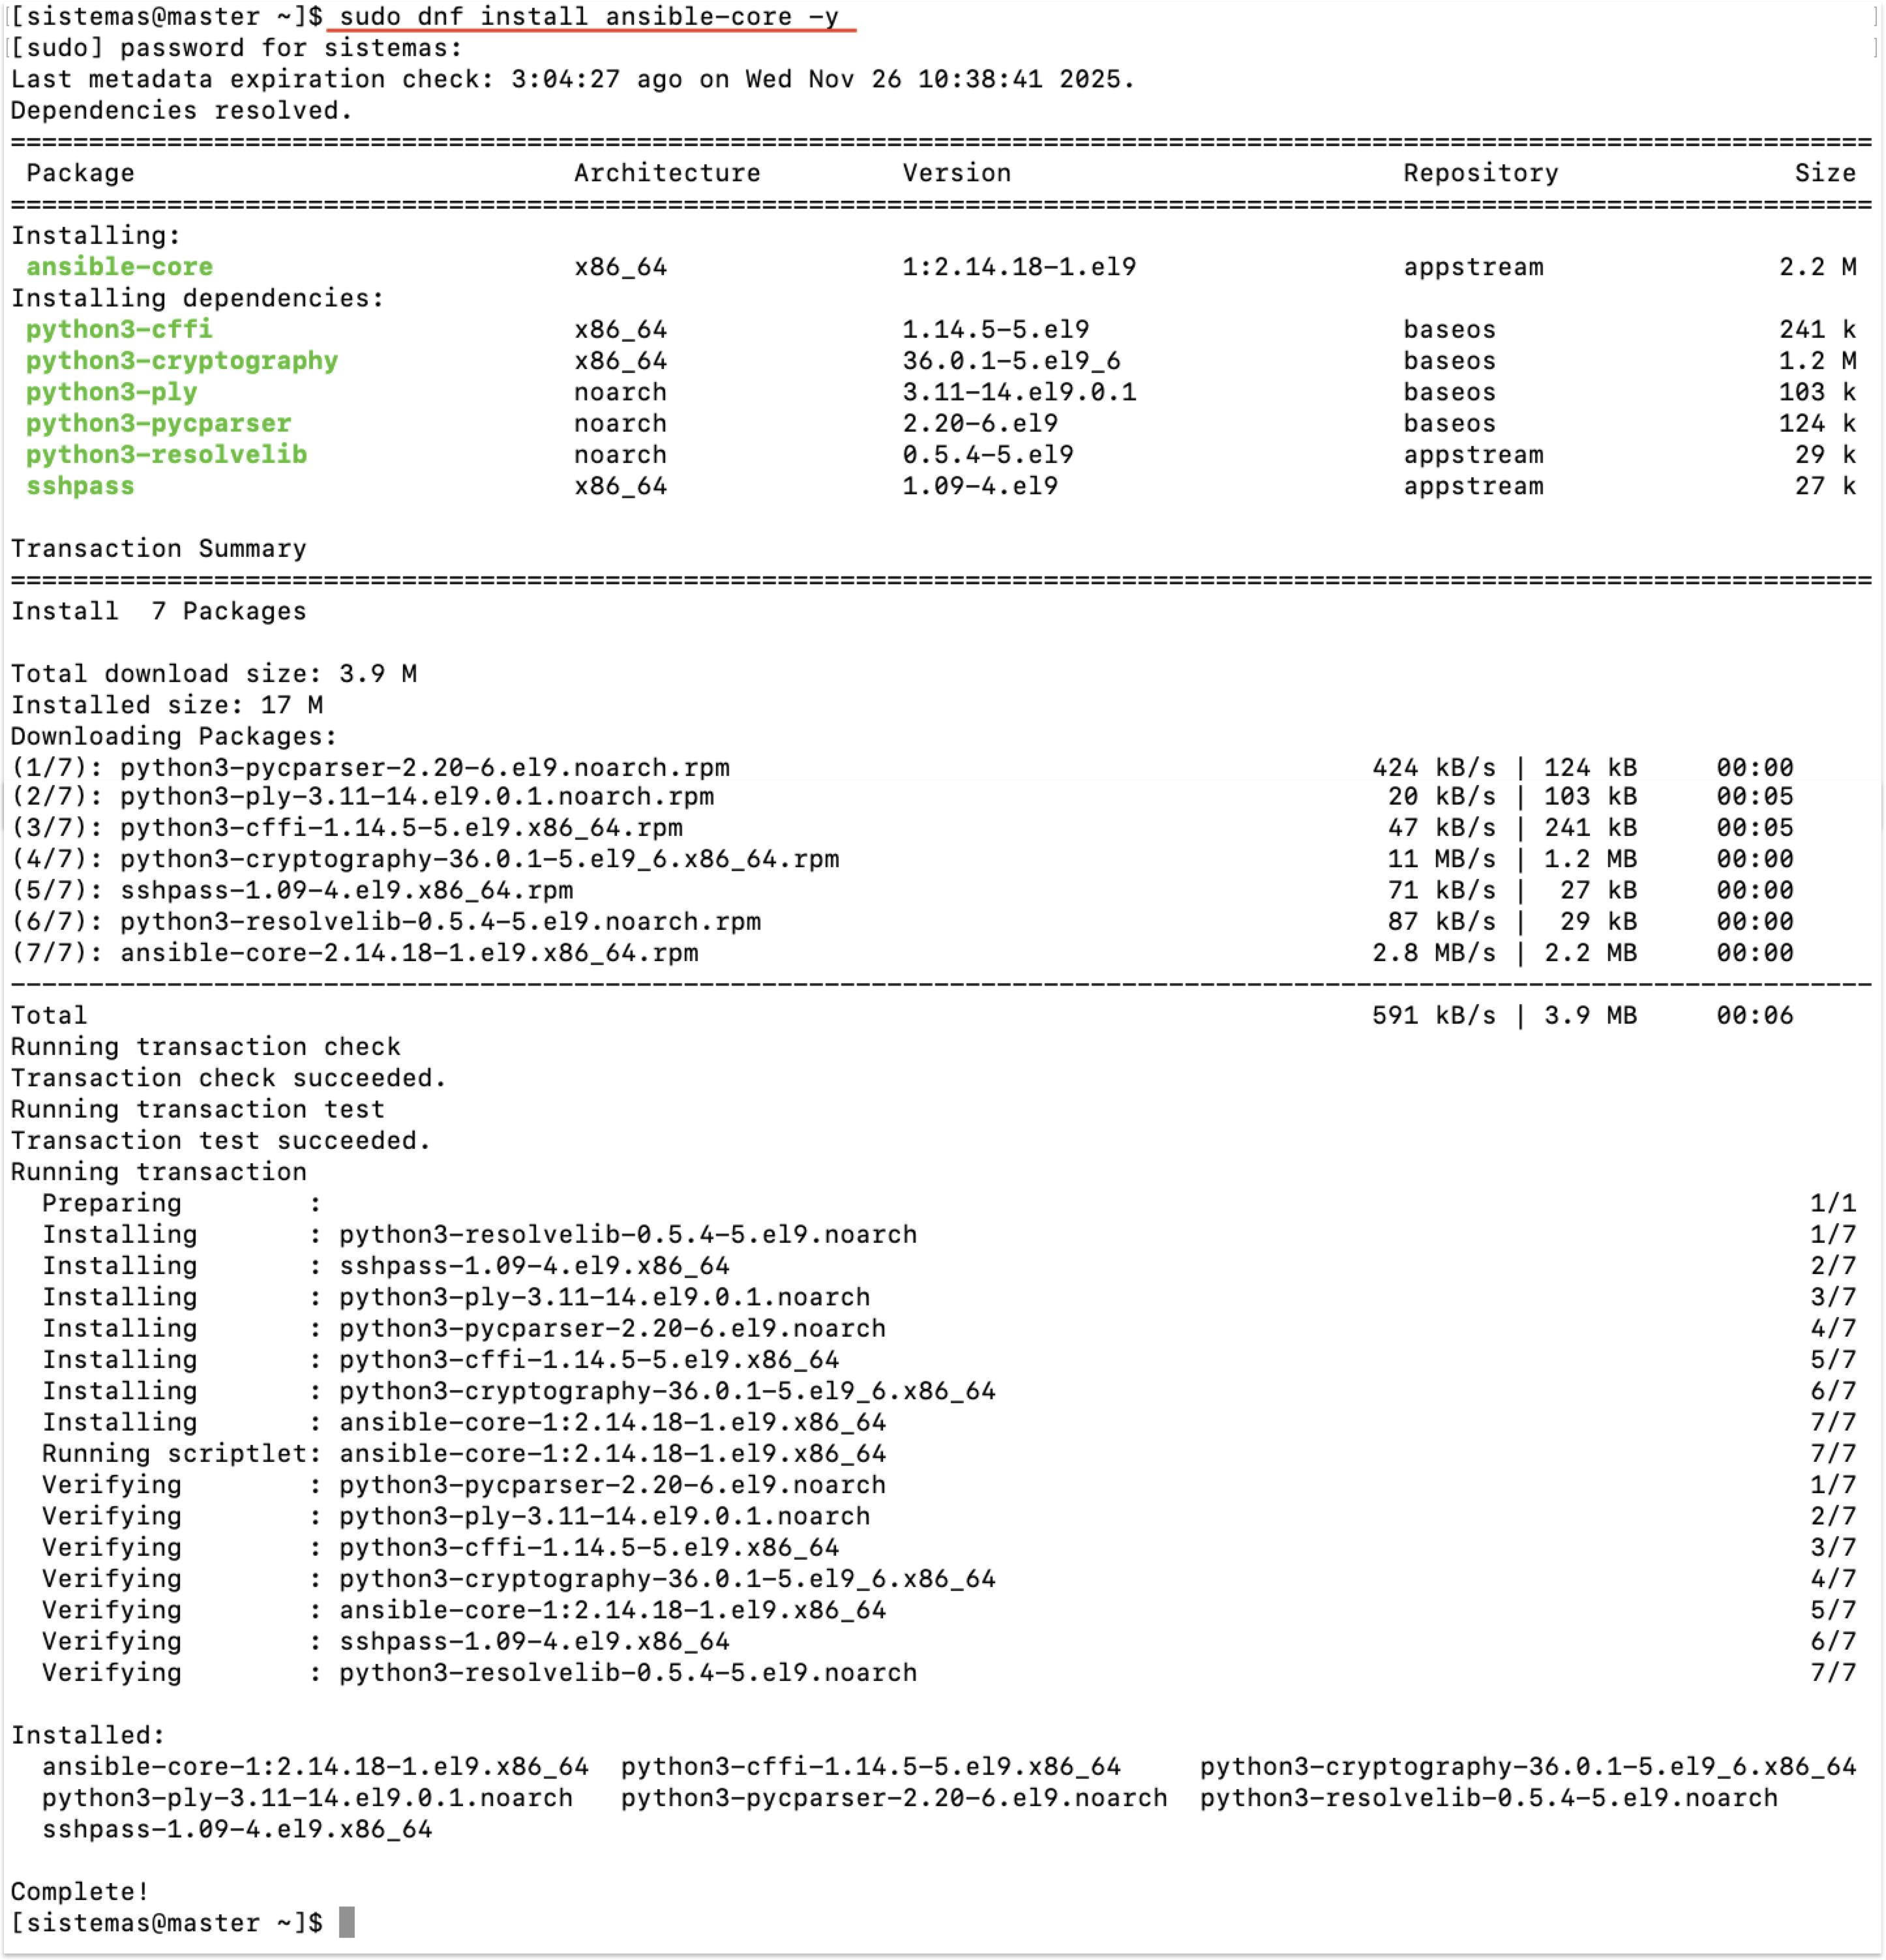
\includegraphics[width=0.6\textwidth]{images/ansible/ansible-core install.png}
  \caption{Instalación de Ansible (paquete \texttt{ansible-core}) en el master.}
  \label{fig:install_ansible_core}
\end{figure}

\begin{enumerate}
  \setcounter{enumi}{2}
  \item Se verificó la instalación y versión:
\end{enumerate}

\begin{verbatim}
ansible --version
\end{verbatim}

La salida mostró la versión de \texttt{ansible-core}, la versión de Python y la ruta del archivo de configuración de Ansible cuando aplica. Esto confirmó que Ansible quedó disponible desde la terminal del \textit{master}. \cite{ansible_installation_guide}

\begin{figure}[h]
  \centering
  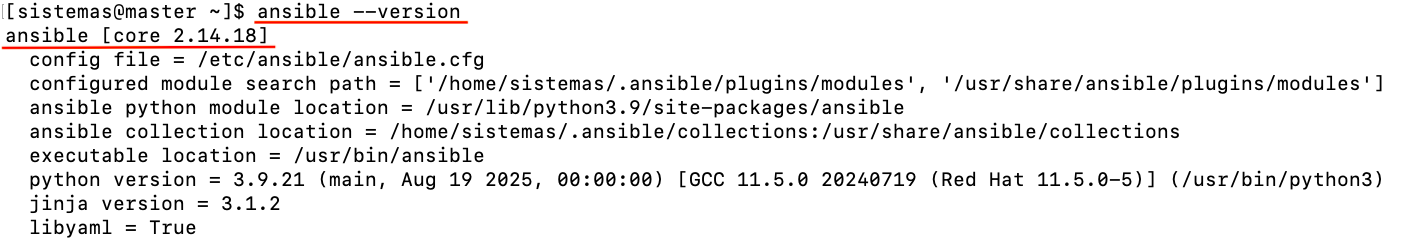
\includegraphics[width=0.92\textwidth]{images/ansible/ansible version.png}
  \caption{Verificación de instalación de Ansible con \texttt{ansible --version}.}
  \label{fig:p03_ansible_version}
\end{figure}

\subsection{Estructura mínima del proyecto de automatización}
\label{subsec:ansible_project_structure}

En este proyecto se organiza la automatización como un directorio de trabajo que contiene:
\begin{itemize}
  \item Un inventario (lista de hosts del clúster).
  \item Una configuración local del proyecto (\texttt{ansible.cfg}) para evitar depender de configuraciones globales.
  \item Playbooks y roles (cuando la automatización crece).
\end{itemize}

Mantener un \texttt{ansible.cfg} local ayuda a que el proyecto sea replicable: quien copie el repositorio obtiene la misma configuración por defecto. Ansible incluye herramientas para inspeccionar configuración y sus fuentes, como \texttt{ansible-config}. \cite{ansible_config_reference}

\subsubsection*{Procedimiento realizado}
\begin{enumerate}
  \item Se creó un directorio de trabajo para la automatización (ejemplo: \texttt{\textasciitilde/hpc-ansible}) y se ingresó a él:
\end{enumerate}

\begin{verbatim}
mkdir -p ~/hpc-ansible
cd ~/hpc-ansible
\end{verbatim}

\begin{figure}[H]
  \centering
  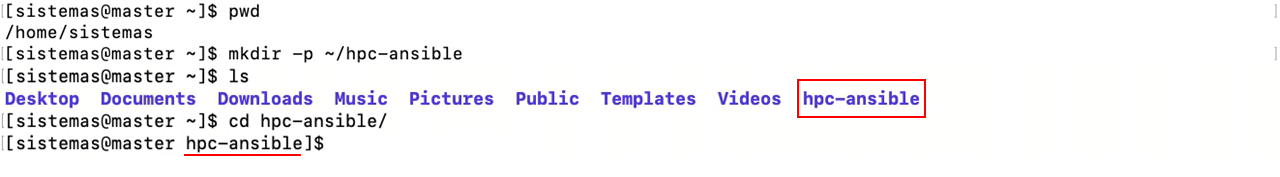
\includegraphics[width=0.92\textwidth]{images/ansible/dir ansible.png}
  \caption{Creación del directorio exclusivo para usar Ansible}
  \label{fig:p04_project_structure}
\end{figure}

\subsection{Creación del inventario del clúster (\texttt{inventario.ini})}
\label{subsec:ansible_inventory_ini_real}

El inventario define qué equipos administra Ansible y cómo conectarse a ellos. En este proyecto se organizó el inventario en dos grupos: \texttt{master} y \texttt{workers}. Además, se definió el usuario remoto común (\texttt{sistemas}) como variable global. \cite{ansible_inventory_intro,ansible_connection_details}

\subsubsection*{Procedimiento realizado}
\begin{enumerate}
  \item Se creó el archivo \texttt{inventario.ini} usando \texttt{nano}:
\end{enumerate}

\begin{verbatim}
nano inventario.ini
\end{verbatim}

En el editor se escribió el siguiente contenido y se guardó el archivo.

\begin{verbatim}
[hpc_master]
master ansible_host=10.195.34.17 ansible_user=sistemas

[workers]
worker1 ansible_host=10.195.20.52 ansible_user=sistemas
worker2 ansible_host=10.195.34.19 ansible_user=sistemas

[all:vars]
ansible_python_interpreter=/usr/bin/python3
ansible_ssh_private_key_file=~/.ssh/id_ed25519
\end{verbatim}

Para guardar en \texttt{nano} se usó \texttt{Ctrl+O}, luego \texttt{Enter}, y para salir \texttt{Ctrl+X}.

\begin{figure}[H]
  \centering
  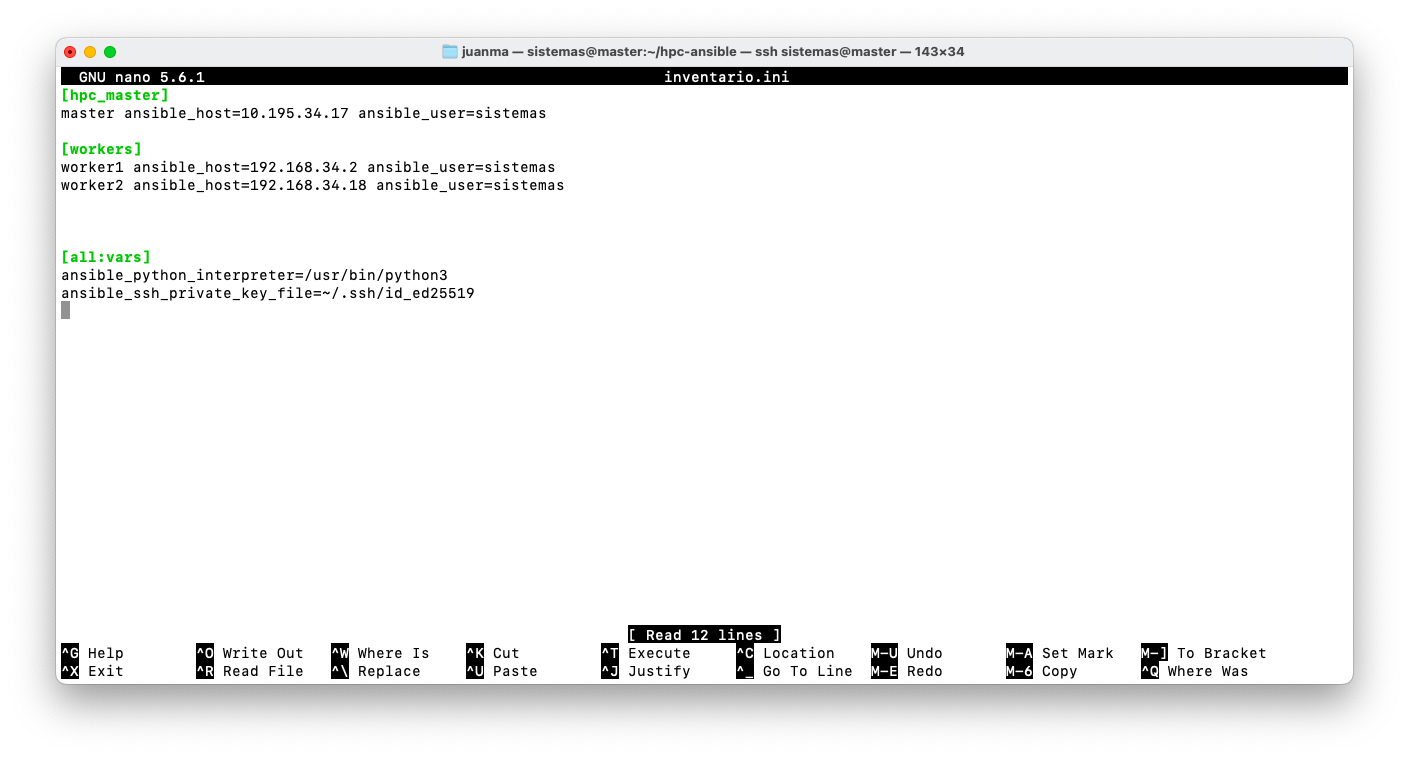
\includegraphics[width=0.92\textwidth]{images/ansible/inventario.png}
  \caption{Edición de \texttt{inventario.ini} con \texttt{nano}.}
  \label{fig:p05_inventory_ini_nano}
\end{figure}

En este punto, \texttt{worker1} y \texttt{worker2} pueden resolverse por nombre si existe DNS o si posteriormente se agregan entradas en \texttt{/etc/hosts}. Si aún no hay resolución de nombres, el inventario se completa asignando \texttt{ansible\_host=<IP>} a cada worker.

\subsection{Configuración local del proyecto (\texttt{ansible.cfg})}
\label{subsec:ansible_cfg_local_minimo}

Ansible permite definir parámetros por defecto en \texttt{ansible.cfg}. En esta fase se utiliza un archivo local para fijar el inventario por defecto y evitar escribir \texttt{-i inventory.ini} en cada comando. La referencia oficial documenta este comportamiento y las opciones disponibles. \cite{ansible_config_reference}

\subsubsection*{Procedimiento realizado}
\begin{enumerate}
  \item Se creó el archivo \texttt{ansible.cfg} usando \texttt{nano}:
\end{enumerate}

\begin{verbatim}
nano ansible.cfg
\end{verbatim}

En el editor se escribió el siguiente contenido y se guardó el archivo:

\begin{verbatim}
[defaults]
inventory = inventario.ini
timeout = 30

[ssh_connection]
pipelining = True
\end{verbatim}

\begin{figure}[H]
  \centering
  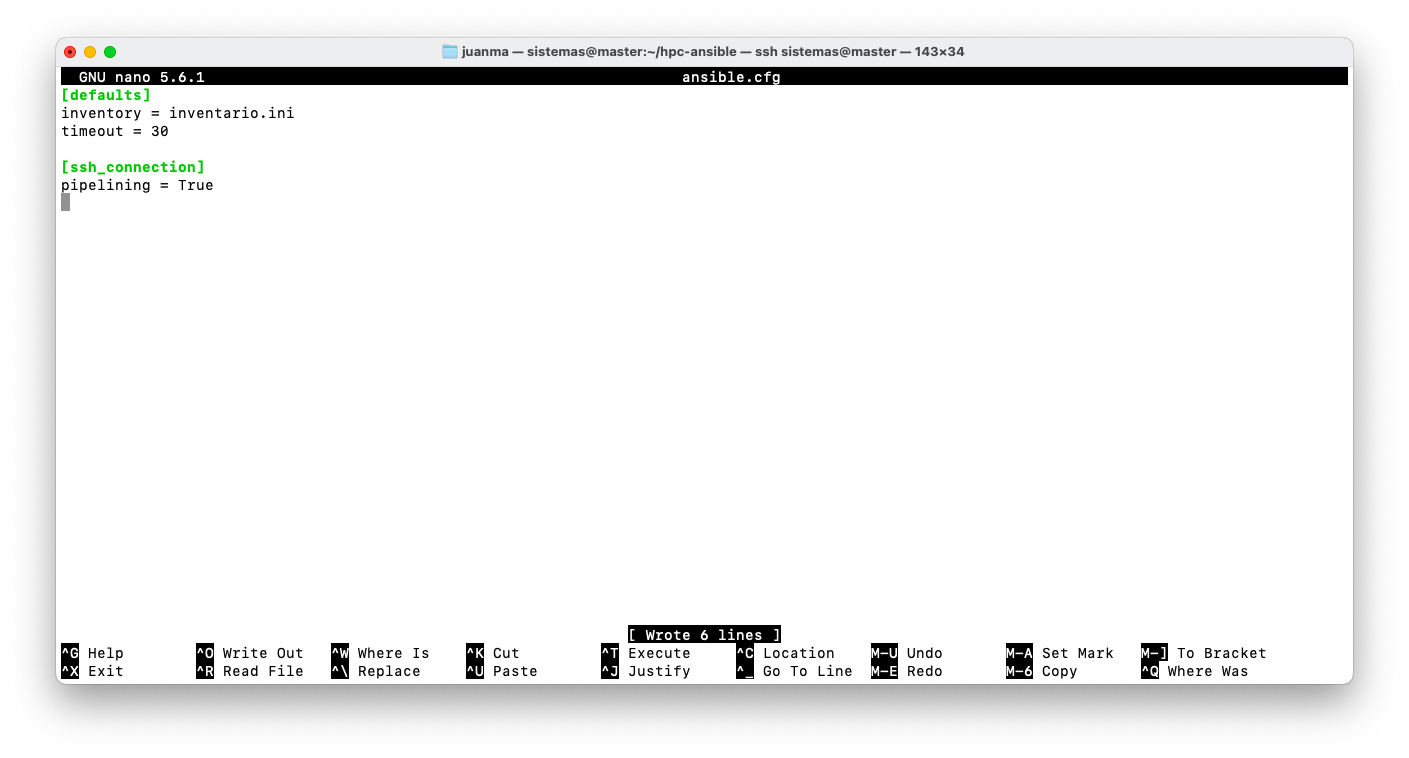
\includegraphics[width=0.92\textwidth]{images/ansible/ansible cfg.png}
  \caption{Edición de \texttt{ansible.cfg} con \texttt{nano}.}
  \label{fig:p06_ansible_cfg_nano}
\end{figure}

\begin{enumerate}
  \setcounter{enumi}{1}
  \item Se verificó que Ansible estuviera usando el archivo de configuración local:
\end{enumerate}

\begin{verbatim}
ansible --version
\end{verbatim}

En la salida se observó la línea \texttt{config file = .../hpc-ansible/ansible.cfg}, lo cual confirmó que la ejecución estaba tomando la configuración del proyecto.

\begin{figure}[H]
  \centering
  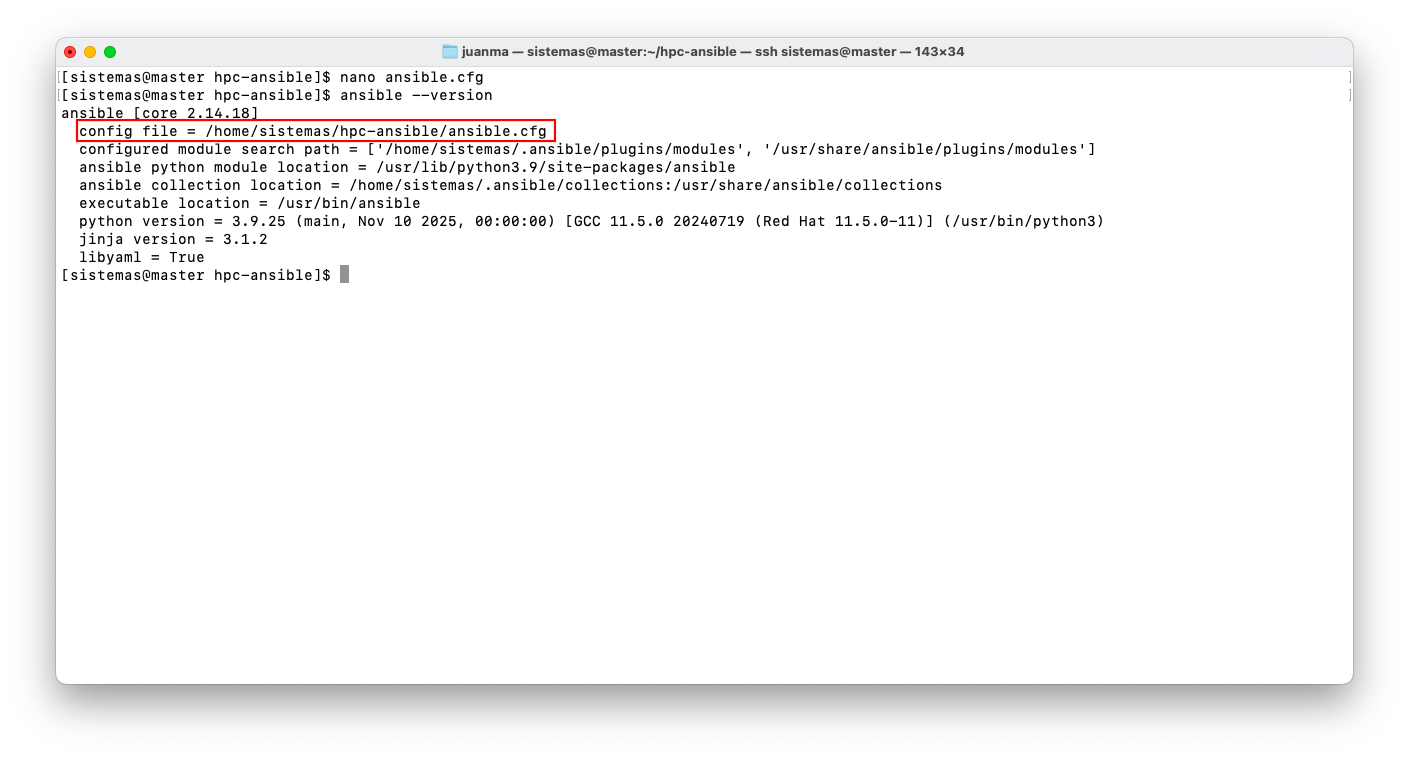
\includegraphics[width=0.92\textwidth]{images/ansible/ansible ver cfg.png}
  \caption{Verificación de \texttt{config file} en \texttt{ansible --version}.}
  \label{fig:p07_ansible_version_config_file}
\end{figure}

\subsection{Primera prueba de conectividad con Ansible}
\label{subsec:ansible_first_ping_minimo}

El módulo \texttt{ping} de Ansible se usa como prueba inicial porque confirma que el nodo de control puede conectarse al host remoto y ejecutar un módulo básico. Esta prueba depende de que exista conectividad SSH y credenciales correctas (preferiblemente llaves). \cite{ansible_adhoc_intro,ansible_connection_details}

\subsubsection*{Procedimiento realizado}
\begin{enumerate}
  \item Se probó conectividad contra todos los hosts del inventario:
\end{enumerate}

\begin{verbatim}
ansible all -m ping
\end{verbatim}

En la salida se observó \texttt{pong} en los hosts accesibles, lo cual confirmó que Ansible podía ejecutar módulos de forma remota.

\begin{figure}[H]
  \centering
  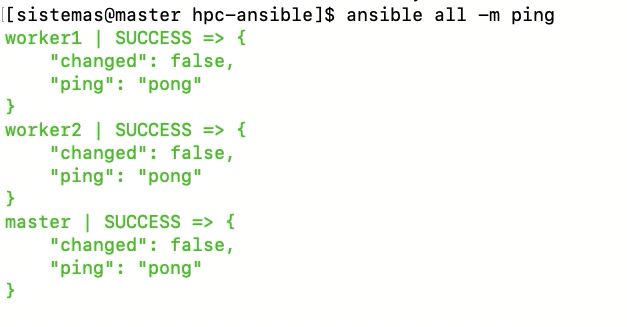
\includegraphics[width=0.75\textwidth]{images/ansible/all ping.png}
  \caption{Primera prueba con \texttt{ansible all -m ping} y respuesta \texttt{pong}.}
  \label{fig:p08_ansible_ping_all}
\end{figure}

\begin{enumerate}
  \setcounter{enumi}{1}
  \item Se verificó la identificación de los workers ejecutando \texttt{hostname}:
\end{enumerate}

\begin{verbatim}
ansible workers -m command -a "hostname"
\end{verbatim}

La salida mostró \texttt{worker1} y \texttt{worker2}, lo cual evidenció que las conexiones estaban llegando a los nodos correctos.

\begin{figure}[H]
  \centering
  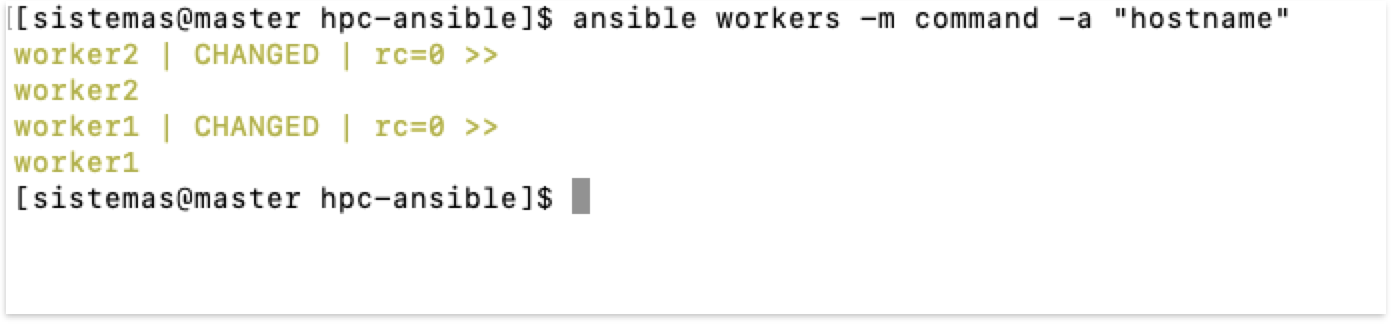
\includegraphics[width=0.92\textwidth]{images/ansible/ansible hostname workers.png}
  \caption{Ejecución del comando \texttt{hostname} en los workers con Ansible.}
  \label{fig:p09_ansible_hostname_workers}
\end{figure}

\section{YAML: el formato base de Ansible}
\label{sec:ansible_yaml}

Antes de describir playbooks, es útil entender \textbf{YAML}, el formato de texto con el que se escriben. YAML está pensado para ser legible por humanos, usando indentación para definir estructura. En Ansible, la mayoría de archivos clave (\texttt{site.yml}, playbooks, variables) están en YAML.

Conceptos mínimos de YAML:
\begin{itemize}
  \item \textbf{Indentación:} define jerarquías. Se recomienda usar dos espacios. No se mezclan tabs.
  \item \textbf{Listas:} comienzan con guion. Cada elemento es un ítem.
  \item \textbf{Mapas (pares clave-valor):} se escriben como \texttt{clave: valor}.
\end{itemize}

Ejemplo simple de YAML (lista de paquetes):
\begin{verbatim}
packages:
  - vim
  - git
  - htop
\end{verbatim}

Y ejemplo con mapas y listas combinadas:
\begin{verbatim}
server:
  name: nodo01
  services:
    - ssh
    - firewalld
\end{verbatim}

En Ansible, un playbook es una \textbf{lista} de \textit{plays}; por eso suele comenzar con un guion. La indentación y los guiones indican la estructura del documento. \cite{ansible_playbooks_intro}

\section{Playbooks, \textit{plays} y tareas (\textit{tasks})}
\label{sec:ansible_playbooks_plays_tasks}

Un \textbf{playbook} es el archivo YAML que describe una secuencia de acciones automatizables. Dentro de un playbook existen uno o varios \textbf{\textit{plays}}. Cada \textit{play} define \textit{qué hosts} se van a configurar, \textit{con qué permisos} y \textit{qué tareas} se ejecutan. Las \textbf{tareas (\textit{tasks})} son la unidad mínima de trabajo y normalmente invocan un módulo de Ansible para llevar un recurso a un estado deseado. \cite{ansible_playbooks_intro,ansible_modules_intro}

Componentes principales de un \textit{play}:
\begin{itemize}
  \item \textbf{name:} descripción en lenguaje natural. Aparece en la salida al ejecutar el playbook.
  \item \textbf{hosts:} grupo de equipos objetivo (por ejemplo, \texttt{all}, \texttt{hpc\_master}, \texttt{workers}).
  \item \textbf{become:} indica si se ejecuta con privilegios elevados (similar a \texttt{sudo}).
  \item \textbf{vars:} variables locales del \textit{play}. Permiten reutilizar el playbook.
  \item \textbf{tasks:} lista ordenada de tareas. Cada tarea invoca un módulo.
  \item \textbf{handlers:} acciones que se ejecutan solo si una tarea notificó cambios.
  \item \textbf{roles:} alternativa para declarar conjuntos de tareas empaquetadas.
\end{itemize}

Componentes principales de una \textit{task}:
\begin{itemize}
  \item \textbf{name:} descripción de la tarea.
  \item \textbf{módulo:} acción concreta (por ejemplo, \texttt{ansible.builtin.dnf}, \texttt{ansible.builtin.copy}).
  \item \textbf{parámetros:} argumentos del módulo, escritos en YAML.
  \item \textbf{notify:} opcional, dispara un \textit{handler} si hubo cambios.
\end{itemize}

Esta estructura permite separar responsabilidades: un \textit{play} puede dedicarse a configurar \textit{workers}, y otro a configurar el \textit{master}. A medida que el proyecto crece, se incorporan \textbf{roles} para encapsular conjuntos de tareas reutilizables.

\subsection{Ejemplo A: playbook con dos \textit{plays}}
\label{subsec:ansible_play_example_two_plays}

El siguiente ejemplo muestra un playbook con dos \textit{plays}: uno para tareas base en todos los nodos y otro específico para un grupo \texttt{web}.

\begin{verbatim}
# multi-play.yml (ejemplo)
- name: Preparar sistema base
  hosts: all
  become: yes
  tasks:
    - name: Ajustar zona horaria
      ansible.builtin.timezone:
        name: America/Bogota
    - name: Instalar paquetes base
      ansible.builtin.dnf:
        name:
          - vim
          - git
        state: present

- name: Configurar servidor web
  hosts: web
  become: yes
  tasks:
    - name: Instalar nginx
      ansible.builtin.dnf:
        name: nginx
        state: present
    - name: Habilitar y arrancar nginx
      ansible.builtin.systemd:
        name: nginx
        enabled: true
        state: started
\end{verbatim}

Aquí se observa que el primer \textit{play} es general (\texttt{all}) y el segundo se limita a un grupo específico (\texttt{web}). Cada \textit{play} puede tener sus propias tareas y variables.

\subsection{Ejemplo B: tareas con \textit{handlers}}
\label{subsec:ansible_play_example_handlers}

Un \textbf{\textit{handler}} es una tarea especial que \textbf{solo se ejecuta si alguna tarea anterior reporta cambios}. Se usa para acciones que no deben repetirse innecesariamente, como reiniciar o recargar un servicio.


Este ejemplo ilustra cómo una tarea puede disparar un \textit{handler} para reiniciar un servicio únicamente si hubo cambios en un archivo:

\begin{verbatim}
# config-app.yml (ejemplo)
- name: Desplegar configuración de una app
  hosts: app
  become: yes
  vars:
    app_port: 8080
  tasks:
    - name: Copiar plantilla de configuración
      ansible.builtin.template:
        src: templates/app.conf.j2
        dest: /etc/app/app.conf
      notify: Reiniciar servicio de app

  handlers:
    - name: Reiniciar servicio de app
      ansible.builtin.systemd:
        name: app
        state: restarted
\end{verbatim}

La relación entre tareas y \textit{handlers} es clave para mantener idempotencia y evitar reinicios innecesarios.

\section{Módulos de Ansible}
\label{sec:ansible_modulos}

Un \textbf{módulo} es la pieza que realiza el trabajo concreto dentro de una tarea. Cuando Ansible ejecuta una tarea, en realidad está llamando a un módulo que sabe cómo \textit{instalar un paquete}, \textit{copiar un archivo}, \textit{crear un usuario} o \textit{gestionar un servicio}. Los módulos están diseñados para ser \textbf{idempotentes}: si el estado deseado ya se cumple, no hacen cambios. \cite{ansible_modules_intro}

Componentes básicos de una tarea con módulo:
\begin{itemize}
  \item \textbf{name:} descripción de la acción.
  \item \textbf{módulo:} el nombre del módulo a ejecutar (por ejemplo, \texttt{ansible.builtin.dnf}).
  \item \textbf{parámetros:} opciones específicas del módulo (por ejemplo, nombre del paquete, estado).
\end{itemize}

Ejemplo de tarea usando un módulo:
\begin{verbatim}
- name: Asegurar que htop esté instalado
  ansible.builtin.dnf:
    name: htop
    state: present
\end{verbatim}

Otros módulos comunes:
\begin{itemize}
  \item \textbf{\texttt{ansible.builtin.copy}} para copiar archivos estáticos.
  \item \textbf{\texttt{ansible.builtin.template}} para generar archivos desde plantillas.
  \item \textbf{\texttt{ansible.builtin.systemd}} para habilitar o reiniciar servicios.
\end{itemize}

Comprender los módulos es clave porque cada uno tiene parámetros propios y resultados distintos. En capítulos posteriores se profundiza en los módulos más usados dentro del clúster.

\section{Playbook principal del proyecto (\texttt{site.yml}): estructura base}
\label{sec:ansible_site_base}

El archivo \texttt{site.yml} es el punto de entrada del proyecto de automatización. En esta etapa se presenta una \textbf{estructura base simplificada} que se irá completando a medida que avanzan los capítulos. Esta versión inicial permite entender la organización general sin entrar aún en todo el detalle.

\begin{verbatim}
# site.yml (estructura base inicial)
- name: Baseline para todos los nodos
  hosts: all
  become: true
  roles:
    - common
    # (se agregan más roles de base en capítulos posteriores)
\end{verbatim}

En los siguientes apartados se muestra cómo esta estructura se va enriqueciendo con roles adicionales hasta llegar a la versión actual del proyecto.


\section{Roles en Ansible}
\label{sec:ansible_roles}

Un \textbf{rol} es una forma de organizar la automatización en una estructura reutilizable y ordenada. En lugar de escribir todas las tareas dentro de un playbook, un rol agrupa tareas, variables, archivos y plantillas relacionadas con un objetivo específico (por ejemplo: \textit{firewall}, \textit{usuarios}, \textit{Slurm}).

Componentes típicos de un rol:
\begin{itemize}
  \item \textbf{\texttt{tasks/}}: lista de tareas principales del rol.
  \item \textbf{\texttt{defaults/}}: variables con valores por defecto (se pueden sobrescribir).
  \item \textbf{\texttt{vars/}}: variables internas del rol (prioridad más alta).
  \item \textbf{\texttt{handlers/}}: tareas especiales que se ejecutan solo si hubo cambios.
  \item \textbf{\texttt{templates/}}: archivos con plantillas Jinja2 para generar configuraciones.
  \item \textbf{\texttt{files/}}: archivos estáticos que se copian tal cual.
\end{itemize}

Cómo se usan los roles:
\begin{itemize}
  \item En un playbook se listan bajo \texttt{roles:} para aplicarlos a un grupo de hosts.
  \item Los roles se ejecutan en el orden en que aparecen.
  \item Las variables permiten adaptar el comportamiento del rol a cada entorno.
\end{itemize}

La ventaja principal es la \textbf{reutilización}: un rol bien definido puede usarse en distintos proyectos o aplicarse a varios grupos de hosts sin reescribir tareas.

\subsection{Ejemplo de rol: estructura y archivos clave}
\label{subsec:ansible_roles_ejemplo}

El siguiente ejemplo muestra un rol sencillo llamado \texttt{mi\_servicio}, con una estructura mínima típica. Se incluye un diagrama ASCII para visualizar las carpetas y dos archivos clave: uno de tareas y otro de \textit{handlers}.

\begin{verbatim}
roles/
└── mi_servicio/
    ├── tasks/
    │   └── main.yml
    ├── handlers/
    │   └── main.yml
    ├── defaults/
    │   └── main.yml
    ├── templates/
    │   └── mi_servicio.conf.j2
    └── files/
        └── banner.txt
\end{verbatim}

Ejemplo de \texttt{tasks/main.yml}:
\begin{verbatim}
# roles/mi_servicio/tasks/main.yml
- name: Instalar paquete del servicio
  ansible.builtin.dnf:
    name: mi-servicio
    state: present

- name: Desplegar configuración
  ansible.builtin.template:
    src: mi_servicio.conf.j2
    dest: /etc/mi_servicio/mi_servicio.conf
  notify: Reiniciar mi servicio
\end{verbatim}

Ejemplo de \texttt{handlers/main.yml}:
\begin{verbatim}
# roles/mi_servicio/handlers/main.yml
- name: Reiniciar mi servicio
  ansible.builtin.systemd:
    name: mi-servicio
    state: restarted
\end{verbatim}

Cómo funciona todo en conjunto:
\begin{itemize}
  \item El playbook invoca el rol \texttt{mi\_servicio} bajo la sección \texttt{roles:}.
  \item Ansible ejecuta las tareas de \texttt{tasks/main.yml} en orden.
  \item Si la tarea de plantilla modifica el archivo de configuración, se activa el \textit{handler}.
  \item El \textit{handler} reinicia el servicio solo cuando hubo cambios, evitando reinicios innecesarios.
\end{itemize}

\section{Variables, plantillas y archivos estáticos}
\label{sec:ansible_vars_templates_files}

Esta sección explica tres conceptos esenciales para hacer playbooks y roles flexibles: \textbf{variables}, \textbf{plantillas} y \textbf{archivos estáticos}. Cada uno cumple un propósito distinto, pero juntos permiten automatizar configuraciones reales sin repetir información.

\subsection{Variables}
\label{subsec:ansible_variables_intro}

Una \textbf{variable} es un valor que puede cambiar sin modificar el playbook. Sirve para parametrizar nombres de paquetes, rutas, puertos o usuarios. En Ansible, las variables se definen en diferentes lugares (por ejemplo, dentro del playbook, en \texttt{group\_vars/}, \texttt{host\_vars/} o en \texttt{defaults/} de un rol) y luego se usan con la sintaxis \texttt{\{\{ variable \}\}}. \cite{ansible_variables}

Ejemplo simple de variables en un playbook:
\begin{verbatim}
- name: Configurar un servicio con variables
  hosts: all
  become: yes
  vars:
    servicio: nginx
    puerto: 8080
  tasks:
    - name: Instalar servicio
      ansible.builtin.dnf:
        name: "{{ servicio }}"
        state: present
\end{verbatim}

En este ejemplo, cambiar \texttt{servicio} o \texttt{puerto} modifica el comportamiento del playbook sin reescribir tareas.

\subsection{Plantillas (Jinja2)}
\label{subsec:ansible_templates_intro}

Una \textbf{plantilla} es un archivo de texto que incluye variables y lógica básica para generar configuraciones dinámicas. Ansible utiliza el motor \textbf{Jinja2} para reemplazar variables y crear un archivo final en el host remoto. El módulo más común es \texttt{ansible.builtin.template}.

Las variables que aparecen en una plantilla provienen de las mismas fuentes que en un playbook: pueden estar definidas en \texttt{vars:} dentro del playbook, en archivos de grupo (\texttt{group\_vars/}), en archivos por host (\texttt{host\_vars/}) o en los \texttt{defaults/} de un rol. Al ejecutar el playbook, Ansible construye un conjunto de variables disponible para la plantilla y reemplaza cada \texttt{\{\{ variable \}\}} con su valor correspondiente. \cite{ansible_variables}

Ejemplo de plantilla (\texttt{templates/app.conf.j2}):
\begin{verbatim}
# app.conf.j2 (ejemplo)
port={{ puerto }}
log_path={{ log_dir }}/app.log
\end{verbatim}

Ejemplo de tarea que renderiza la plantilla:
\begin{verbatim}
- name: Generar configuración desde plantilla
  ansible.builtin.template:
    src: templates/app.conf.j2
    dest: /etc/mi_app/app.conf
\end{verbatim}

Si cambian las variables \texttt{puerto} o \texttt{log\_dir}, el archivo generado será diferente. Esto permite mantener una sola plantilla para múltiples nodos con configuraciones específicas.

\subsection{Archivos estáticos}
\label{subsec:ansible_static_files}

Un \textbf{archivo estático} es un archivo que se copia exactamente igual al host remoto, sin reemplazo de variables. Se usa para binarios, scripts, certificados, o archivos de texto que no requieren personalización. El módulo típico es \texttt{ansible.builtin.copy}, y los archivos suelen vivir en la carpeta \texttt{files/} del rol.

Ejemplo de tarea con archivo estático:
\begin{verbatim}
- name: Copiar banner estático
  ansible.builtin.copy:
    src: banner.txt
    dest: /etc/issue
    owner: root
    group: root
    mode: "0644"
\end{verbatim}

Es importante que la ruta de destino exista en los nodos de destino (por ejemplo, \texttt{/etc/} o \texttt{/opt/mi\_app/}). Si el directorio no existe, la tarea fallará, por lo que normalmente se crea antes con un módulo como \texttt{ansible.builtin.file}.

\section{Ejecución de playbooks y lectura de resultados}
\label{sec:ansible_ejecucion_playbooks}

Una vez escrito un playbook, se ejecuta con el comando \texttt{ansible-playbook}. El objetivo es que Ansible lea el archivo, se conecte a los hosts definidos en el inventario, ejecute las tareas en orden y reporte el resultado de cada una.

Comando general de ejecución:
\begin{verbatim}
ansible-playbook -i inventory.ini mi-playbook.yml
\end{verbatim}

Componentes del comando:
\begin{itemize}
  \item \textbf{\texttt{ansible-playbook}}: ejecuta playbooks.
  \item \textbf{\texttt{-i inventory.ini}}: indica el inventario a usar.
  \item \textbf{\texttt{mi-playbook.yml}}: el archivo con los \textit{plays} y tareas.
\end{itemize}

Si el proyecto ya tiene un \texttt{ansible.cfg} con el inventario por defecto, la opción \texttt{-i} puede omitirse. También es común usar \texttt{--limit} para restringir la ejecución a un host o grupo (por ejemplo, un solo worker durante pruebas).

\subsection{¿Qué muestra la salida de Ansible?}
\label{subsec:ansible_output}

Durante la ejecución, Ansible imprime una línea por cada tarea, junto con su estado. Los estados más comunes son:
\begin{itemize}
  \item \textbf{\texttt{ok}}: la tarea ya estaba en el estado deseado y no hubo cambios.
  \item \textbf{\texttt{changed}}: la tarea realizó cambios en el sistema.
  \item \textbf{\texttt{failed}}: la tarea falló (se detiene la ejecución salvo que se indique lo contrario).
  \item \textbf{\texttt{skipped}}: la tarea se omitió por una condición o por \texttt{--limit}.
\end{itemize}

Al final, Ansible muestra un resumen (\textit{play recap}) por cada host, indicando cuántas tareas fueron \texttt{ok}, \texttt{changed}, \texttt{failed}, \texttt{skipped}, \texttt{rescued} e \texttt{ignored}. Este resumen permite validar rápidamente si la ejecución fue correcta.

\subsection{Resultado esperado}
\label{subsec:ansible_expected_results}

En una ejecución exitosa, se espera:
\begin{itemize}
  \item Conectividad estable con todos los hosts del inventario.
  \item Cero fallos (\texttt{failed=0}) en el resumen final.
  \item Cambios solo cuando son necesarios (idempotencia).
\end{itemize}

Si se ejecuta el mismo playbook por segunda vez sin modificar nada, la mayoría de tareas deberían aparecer como \texttt{ok} y no \texttt{changed}, lo cual indica que el sistema ya está en el estado deseado.


\clearpage
\addcontentsline{toc}{chapter}{Referencias}
\printbibliography
\end{document}
